
\chapter{Journaux authentifiés tronqués}\label{ch:pruned-log}

\minitoc{}
\clearpage

Dans le \autoref{ch:problematic} nous avons vu que la réplication optimiste d'un contenu et la modification concurrente de ce contenu conduisent à la divergence des copies du contenu.
Les protocoles de réplication sont responsables de la convergence des copies.
La convergence des copies des pairs est une propriété essentielle d'un système collaboratif.
Si les copies des pairs ne sont pas capables de converger, les pairs ne disposent pas du même contexte pour collaborer.
Ce qui peut conduire à des incompréhensions et à l'échec de la collaboration.

Un individu peut trouver un intérêt à perturber, voire compromettre le succès d'une collaboration.
Nous nous intéressons en particulier à un individu qui cherche à compromettre la convergence des copies.
Cet individu est l'adversaire de la collaboration.
Pour atteindre ses objectifs, l'adversaire contrôle le réseau et un ensemble de pairs que nous qualifions de \emph{mal-intentionnés}.
Les pairs qui ne sont pas sous le contrôle de l'adversaire sont qualifiés d'\emph{honnêtes}.

La présence de pairs mal-intentionnés représente un défi.
Ils peuvent exposer des comportements mal-intentionnés difficiles à détecter et déjouer.
Ils peuvent en particulier produire des \emph{équivoques}.
Une équivoque consiste à transmettre à différents pairs des modifications distinctes qui sont perçues comme identiques par le protocole de réplication.
Les copies des pairs honnêtes divergent alors de manière permanente sans qu'ils s'en rendent compte.

Pour détecter les équivoques et intégrer à leur copie l'ensemble des modifications effectuées sur le contenu, les pairs peuvent répliquer un \emph{journal authentifié}.
Chaque pair possède un journal dans lequel il enregistre l'ensemble des modifications qu'il intègre à sa copie du contenu partagé.
Une modification est accompagnée d'une signature cryptographique qui permet de s'assurer de son authenticité.
Un pair mal-intentionné ne peut donc pas prétendre qu'une de ses modifications a été effectuée par un pair honnête.
Un journal authentifié contient uniquement des modifications authentiques.

\begin{figure}[hbt]
\centering
\begin{subfigure}{0.49\linewidth}
    \centering
    \begin{tikzpicture}
        % devices
        \path (0,0)
            to +(190:2) node[
                label=below:{Alice},
                label={[shift={(0,0.7)}]left:{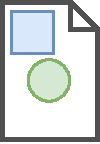
\includegraphics[scale=0.5]{collab/doc-a1-b1.pdf}}},
                label={[shift={(-0.1,-0.7)}]left:{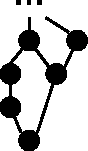
\includegraphics[scale=0.5]{fig/collab/log-sample.pdf}}}
            ](A){
\includegraphics[scale=0.6]{collab/device.pdf}}
            to +(70:2) node[
                label=above:{Bea},
                label={[shift={(0,0.7)}]right:{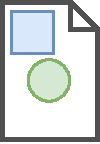
\includegraphics[scale=0.5]{collab/doc-a1-b1.pdf}}},
                label={[shift={(0.1,-0.7)}]right:{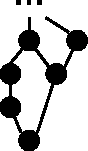
\includegraphics[scale=0.5]{fig/collab/log-sample.pdf}}}
            ](B){
\includegraphics[scale=0.6]{collab/device.pdf}}
            to +(-50:2) node[
                label=below:{Carol}
            ](C){
\includegraphics[scale=0.6]{collab/device.pdf}};
        % Links
        \draw (A) edge[link] (B);
        \draw (B) edge[link] (C);
        \draw (A) edge[link,-latex] node[midway]{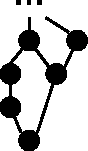
\includegraphics[scale=0.5]{fig/collab/log-sample.pdf}} (C);
    \end{tikzpicture}
    \caption{}\label{fig:invite-by-log-1}
\end{subfigure}
\begin{subfigure}{0.49\linewidth}
\centering
    \begin{tikzpicture}
        % devices
        \path (0,0)
            to +(190:2) node[
                label=below:{Alice},
                label={[shift={(0,0.7)}]left:{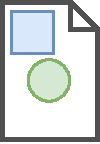
\includegraphics[scale=0.5]{collab/doc-a1-b1.pdf}}},
                label={[shift={(-0.1,-0.7)}]left:{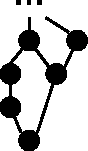
\includegraphics[scale=0.5]{fig/collab/log-sample.pdf}}}
            ](A){
\includegraphics[scale=0.6]{collab/device.pdf}}
            to +(70:2) node[
                label=above:{Bea},
                label={[shift={(0,0.7)}]right:{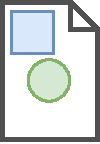
\includegraphics[scale=0.5]{collab/doc-a1-b1.pdf}}},
                label={[shift={(0.1,-0.7)}]right:{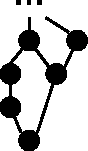
\includegraphics[scale=0.5]{fig/collab/log-sample.pdf}}}
            ](B){
\includegraphics[scale=0.6]{collab/device.pdf}}
            to +(-50:2) node[
                label=below:{Carol},
                label={[shift={(0,0.7)}]right:{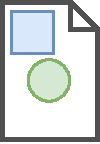
\includegraphics[scale=0.5]{collab/doc-a1-b1.pdf}}},
                label={[shift={(0.1,-0.7)}]right:{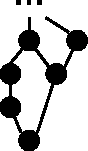
\includegraphics[scale=0.5]{fig/collab/log-sample.pdf}}}
            ](C){
\includegraphics[scale=0.6]{collab/device.pdf}};
        % Links
        \draw[link] (A) to (B);
        \draw[link] (B) to (C);
        \draw[link] (C) to (A);
    \end{tikzpicture}
    \caption{}\label{fig:invite-by-log-2}
\end{subfigure}
\caption[Transmission d'un journal complet à une nouvelle collaboratrice]{Alice et Bea répliquent de manière optimiste un dessin.
Ils utilisent un journal authentifié pour assurer la convergence des copies des pairs honnêtes.
Carol veut rejoindre la collaboration.
\subref{fig:invite-by-log-1} Alice envoie son journal à Carol.
\subref{fig:invite-by-log-2} Carol vérifie l'authenticité du journal et construit le dessin à partir du journal.}\label{fig:invite-by-log}
\end{figure}

Les pairs doivent préserver l'intégralité de leur journal pour \begin{inlinelist}
\item détecter les équivoques et
\item permettre à un pair de rejoindre la collaboration
\end{inlinelist}.
Un pair qui rejoint la collaboration a en effet besoin du journal pour obtenir l'état actuel du contenu partagé.
Il obtient cet état en intégrant sur sa copie vierge du contenu partagé chaque modification enregistrée dans le journal.
La \autoref{fig:invite-by-log} illustre la transmission d'un journal authentifié à un pair qui rejoint la collaboration.
La préservation de l'intégralité du journal engendre plusieurs problèmes~:

\paragraph{Passage à l'échelle.} Au fur et à mesure de la progression de la collaboration, les journaux contiennent de plus en plus de modifications.
La préservation de l'intégralité d'ub journal et leur transmission aux pairs qui rejoignent la collaboration sont donc de plus en plus coûteuses.

\paragraph{Vie Privée.} La préservation du journal dans son intégralité expose l'historique de la collaboration depuis son commencement.
Bien que certaines applications requièrent cette historique pour fournir des fonctionnalités, telle que la visualisation interactive de l'évolution d'un contenu, il peut être intéressant d'offrir plus de liberté sur quelles données doivent être conservées et quelles données doivent être supprimées.

\paragraph{} Pour répondre à ces deux problématiques nous effectuons deux observations~:
\begin{itemize}
    \item Toutes les modifications ne sont pas forcément nécessaires à la détection d'équivoques.
    \item L'occupation mémoire de la copie du contenu partagé est généralement plus fiable que celle du journal.
\end{itemize}

Nous proposons ainsi deux mécanismes~:

\paragraph{Troncature du journal.} Au lieu de préserver l'intégralité du journal, seules les modifications nécessaires à la détection d'équivoques pourraient être conservées.
Pour supprimer une modification du journal nous devons nous assurer qu'elle n'est pas nécessaire à la détection des équivoques futures.
Pour ce faire, nous utilisons des journaux authentifiés dans lesquels chaque modification déclare des dépendances sur d'autres modifications.
Les dépendances sont déclarées de telle manière à résister aux équivoques.
En d'autres termes, si un pair mal-intentionné effectue une équivoque en générant deux modifications $x$ et $y$ et qu'une modification $z$ déclare dépendre de $x$, alors nous considérons qu'il n'est pas possible de prétendre que $z$ dépend de $y$.
Les modifications et leurs dépendances forment ainsi un graphe dirigé sans cycle.
Nous contraignons l'acceptation de modifications dans un journal de telle manière à ce que les modifications acceptées ultérieurement partagent un ensemble croissant de dépendances.
Nous déterminons cet ensemble à l'aide du concept de \emph{stabilité}.
Au sein d'un journal, une modification devient \emph{stable} une fois que toutes les modifications acceptées ultérieurement dans le journal dépendent de cette modification.
Nous proposons un protocole qui permet de supprimer un sous-ensemble des modifications stables.
Lorsque des modifications sont supprimées du journal nous disons que le journal est \emph{tronqué}.
La \autoref{fig:log-example} donne un exemple d'un journal et d'une version tronquée de ce journal.

\begin{figure}[hbt]
\centering
\begin{tikzpicture}
    \newcommand*\hsep{2}
    \path node (a1) {$a_1$}
        to +(\hsep,0) node (a2) {$a_2$}
        to +(2*\hsep,0) node (b1) {$b_1$}
        to +(3*\hsep,0) node (a3) {$a_3$}
        to +(4*\hsep,0) node (b2) {$b_2$}
        to +(5*\hsep,0) node (a4) {$a_4$}
    ;
    % Dependency
    \foreach \src/\dest in {a1/a2,b1/a3,a3/b2,b2/a4}
        \draw[pre] (\src) to node[above,sloped](\src\dest){\footnotesize dep} (\dest);
    \draw[vis,bend right=30] (a1) to node[below,sloped]{\footnotesize dep} (b1);
    \draw[vis,bend left=30] (a2) to node[above,sloped]{\footnotesize dep} (a3);
    % pruned
    \node[draw,dashed,fit=(b2) (b2a4) (a4)]{};
\end{tikzpicture}
\caption[Exemple du journal d'un pair]{Exemple du journal d'un pair.
L'arrangement horizontal des opérations traduit leur ordre d'ajout dans le journal.
Ainsi les opérations ont été ajoutées dans l'ordre suivant~: $a_1$, $a_2$, $b_1$, $a_3$, $b_2$, $a_4$.
Un arc dirigé entre deux modifications se traduit par  \enquote{est une dépendance de}.
La partie entourée correspond à une version tronquée de ce journal.
}\label{fig:log-example}
\end{figure}

\paragraph{Transmission d'un état authentifiable.} Au lieu de récupérer un journal dans son intégralité, un pair qui rejoint une collaboration pourrait récupérer l'état actuel d'une copie du contenu partagé.
Un pair mal-intentionné peut construire un état de toutes pièces avant de le transmettre à un pair qui rejoint la collaboration.
Le nouveau pair n'a aucun moyen de décider si l'état qu'il reçoit est authentique ou falsifié.
Pour s'assurer de l'authenticité d'un état nous proposons un protocole qui permet d'authentifier un état à partir d'un journal tronqué.
Lorsqu'un pair rejoint la collaboration il récupère un état ainsi que le journal tronqué qui lui est associé.
La \autoref{fig:invite-by-snaplog} illustre cette approche.

\paragraph{} Nous développons d'abord le concept de stabilité dans la \autoref{sec:stability}.
Dans la \autoref{sec:full-log-protocol}, nous présentons un protocole qui protége la convergence des copies à l'aide de journaux intégrales.
Nous nous basons sur ce protocole pour présenter dans la \autoref{sec:pruned-log-protocol} un protocole qui permet de tronquer un journal et d'authentifier un état à partir d'un journal tronqué.

\begin{figure}[htb]
\centering
\begin{subfigure}{0.49\linewidth}
    \centering
    \begin{tikzpicture}
        % devices
        \path (0,0)
            to +(190:2) node[
                label=below:{Alice},
                label={[shift={(0,0.7)}]left:{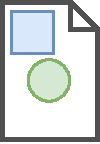
\includegraphics[scale=0.5]{collab/doc-a1-b1.pdf}}},
                label={[shift={(-0.1,-0.7)}]left:{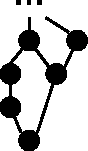
\includegraphics[scale=0.5]{fig/collab/log-sample.pdf}}}
            ](A){
\includegraphics[scale=0.6]{collab/device.pdf}}
            to +(70:2) node[
                label=above:{Bea},
                label={[shift={(0,0.7)}]right:{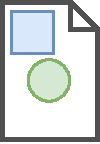
\includegraphics[scale=0.5]{collab/doc-a1-b1.pdf}}},
                label={[shift={(0.1,-0.7)}]right:{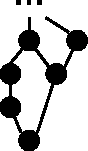
\includegraphics[scale=0.5]{fig/collab/log-sample.pdf}}}
            ](B){
\includegraphics[scale=0.6]{collab/device.pdf}}
            to +(-50:2) node[
                label=below:{Carol}
            ](C){
\includegraphics[scale=0.6]{collab/device.pdf}};
        % Links
        \draw (A) edge[link] (B);
        \draw (B) edge[link] (C);
        \draw (A) edge[link,-latex] node[midway,below]{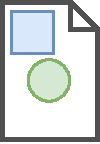
\includegraphics[scale=0.5]{collab/doc-a1-b1.pdf}} node[midway,above]{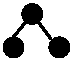
\includegraphics[scale=0.5]{fig/collab/pruned-log.pdf}} (C);
    \end{tikzpicture}
    \caption{}\label{fig:invite-by-snaplog-1}
\end{subfigure}
\begin{subfigure}{0.49\linewidth}
\centering
    \begin{tikzpicture}
        % devices
        \path (0,0)
            to +(190:2) node[
                label=below:{Alice},
                label={[shift={(0,0.7)}]left:{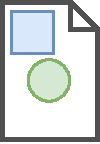
\includegraphics[scale=0.5]{collab/doc-a1-b1.pdf}}},
                label={[shift={(-0.1,-0.7)}]left:{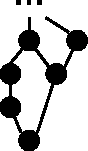
\includegraphics[scale=0.5]{fig/collab/log-sample.pdf}}}
            ](A){
\includegraphics[scale=0.6]{collab/device.pdf}}
            to +(70:2) node[
                label=above:{Bea},
                label={[shift={(0,0.7)}]right:{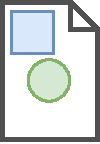
\includegraphics[scale=0.5]{collab/doc-a1-b1.pdf}}},
                label={[shift={(0.1,-0.7)}]right:{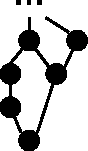
\includegraphics[scale=0.5]{fig/collab/log-sample.pdf}}}
            ](B){
\includegraphics[scale=0.6]{collab/device.pdf}}
            to +(-50:2) node[
                label=below:{Carol},
                label={[shift={(0,0.5)}]right:{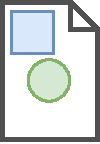
\includegraphics[scale=0.5]{collab/doc-a1-b1.pdf}}},
                label={[shift={(0.2,-0.5)}]right:{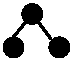
\includegraphics[scale=0.5]{fig/collab/pruned-log.pdf}}}
            ](C){
\includegraphics[scale=0.6]{collab/device.pdf}};
        % Links
        \draw (A) edge[link] (B);
        \draw (B) edge[link] (C);
        \draw (C) edge[link] (A);
    \end{tikzpicture}
    \caption{}\label{fig:invite-by-snaplog-2}
\end{subfigure}
\caption[Transmission d'un journal tronqué et d'un état à une nouvelle collaboratrice]{Alice et Bea répliquent de manière optimiste un dessin.
Ils utilisent un journal authentifié pour assurer la convergence des copies des pairs honnêtes.
Carol veut rejoindre la collaboration.
\subref{fig:invite-by-log-1} Alice envoie l'état actuel de sa copie du dessin, ainsi qu'une version tronquée de son journal authentifié.
\subref{fig:invite-by-log-2} Carol vérifie l'authenticité du journal tronqué.
Elle vérifie également l'authenticité de l'état reçu à partir du journal tronqué.}\label{fig:invite-by-snaplog}
\end{figure}



% Une manière de réduire ce coût est de conserver seulement les opérations les plus récentes.
% Ces opérations forment un suffixe du journal original.
% Nous disons que le journal est tronqué.
% La troncature du journal permet à l'adversaire de la collaboration de mener de nouvelles attaques en vue de faire diverger les copies des pairs honnêtes.
% La suppression de modification du journal peut en effet compromettre la détection d'équivoques.
% Pouvons-nous concevoir un protocole qui permet la troncature du journal sans compromettre la convergence des copies~?

% Une observation importante est que toutes les modifications ne sont pas nécessaires à la détection des équivoques et au maintien de la cohérence du journal.
% En posant des contraintes sur l'acceptation des modifications dans le journal nous pouvons construire un préfixe croissant de modifications du journal qui ne sont plus nécessaires au maintien de la cohérence du journal et à la détection d'équivoques.

% La suppression de modifications du journal se base sur le concept de stabilité que nous développons dans la \autoref{sec:stability}.
% La \autoref{sec:protocole-overview} donne un aperçu du protocole à journaux tronqué que nous présentons dans la \autoref{sec:full-log-protocol} et la \autoref{sec:pruned-log-protocol}.

%Un pair honnête ne peut pas tronquer son journal de manière arbitraire sans menacer la cohérence future de son journal ou la convergence de son journal avec journaux des autres pairs honnêtes.
%La cohérence d'un journal est conservée en vérifiant systématiquement les opérations qui sont reçues.

%Un journal ne peut être arbitrairement tronqué sans menacer la cohérence future du journal ou sa convergence avec les autres journaux.
%Une opération est ajoutée dans un journal cohérent, si elle ne rend pas ce dernier incohérent.
%Cette vérification requiert la présence d'un certain nombre d'opérations qui dépendent du modèle de cohérence considéré.
%Par exemple, pour vérifier une opération dans un journal qui respecte le modèle de cohérence PRAM (ou FIFO), seule l'opération précédente du même auteur est requise.
%Si des opérations nécessaires à la vérification d'une opération sont manquantes, l'opération ne peut être vérifiée.
%L'opération doit donc être rejetée ou intégrée dans le journal avec le risque de le rendre incohérent.
%Pour conserver un journal cohérent, le rejet semble donc le choix le plus judicieux.
%Cependant, elle peut conduire à une divergence permanente des journaux.
%Certains journaux peuvent avoir vérifié et intégré des opérations, e d'autres peuvent les avoir rejetées parce qu'elles ne peuvent pas être vérifiées.
%
%Afin de maintenir un journal cohérent et convergent, les pairs doivent conserver les opérations nécessaires à la vérification de toutes nouvelles opérations.
%Pour supprimer des opérations nous devons donc rencontrer deux conditions~: les opérations nécessaires à la vérification d'une opération devraient représenter un sous-ensemble du journal, et la collaboration devrait progresser de telle manière qu'un préfixe croissant d'opérations n'est plus nécessaire pour vérifier toutes nouvelles opérations.
%Ces deux contraintes peuvent être atteintes en utilisant un modèle de cohérence.
%Un modèle de cohérence restreint la manière dont peuvent être mises en relation deux opérations.
%La concurrence entre opérations joue un rôle important dans la détermination des opérations qui peuvent être ôtées du journal.
%Nous disons qu'une opération est stable une fois qu'il n'est plus possible d'intégrer dans le journal une opération qui lui est concurrente.
%
%Dans un premier temps nous explorons la stabilisation de journaux de manière itératif. dans un second temps, nous utilisant la notion de stabilité pour définir qu'elle partie d'un journal peut être tronquée sans menacer sa cohérence future ou sa convergence avec les autres journaux.


% \section{Aperçu}\label{sec:protocole-overview}

% La convergence à terme des copies est une propriété essentielle des infrastructures pair-à-pair de collaboration.
% Des pairs mal-intentionnés peuvent trouver un intérêt à compromettre la convergence des copies des pairs honnêtes.
% Pour empêcher de tels scénarios, les pairs honnêtes peuvent maintenir un journal authentifié et répliqué.
% Ils enregistrent l'ensemble de leurs modifications dans leur journal respectif.
% Les pairs synchronisent leurs journaux afin de récupérer et intégrer sur leur copie les modifications de chacun.

% Chaque pair doit conserver l'intégralité de son journal pour \begin{inlinelist}
%     \item vérifier la cohérence du journal lors de l'ajout d'une nouvelle opération
%     \item permettre à de nouveaux pairs de rejoindre la collaboration
% \end{inlinelist}.
% Les nouveaux pairs jouent les opérations enregistrées dans le journal pour obtenir le document partagé.
% La \autoref{fig:invite-by-log} montre que les nouveaux pairs utilisent le journal pour obtenir le document partagé.
% Pour ce faire, ils intègrent les modifications enregistrées dans le journal.
% La préservation de l'intégralité du journal engendre plusieurs problèmes~:

% \paragraph{Passage à l'échelle.} Au fur et à mesure de la progression de la collaboration les journaux contiennent de plus en plus d'entrées.
% La préservation des journaux et leur transmission aux pairs qui rejoignent la collaboration sont donc de plus en plus coûteuses.

% \paragraph{Vie Privée.} La préservation du journal dans son intégralité expose l'historique de la collaboration depuis son commencement.
% Bien que certaines applications requièrent cette historique pour fournir des fonctionnalités, telle que la visualisation interactive de l'évolution d'un document, il peut être intéressant d'offrir plus de liberté sur quelles données doivent être conservées et quelles données doivent être supprimées.

% \bigskip

% Un journal enregistre l'ensemble des modifications qui ont été intégrées à un contenu partagé.
% Un contenu est souvent plus petit que le journal qui lui est attaché.
% Certaines applications prennent avantage de cette observation.
% Au lieu de transmettre un journal à un nouveau pair, elles transmettent un instantané du document.

% Notre contexte ne nous permet pas d'adopter cette approche.
% En effet, un pair mal-intentionné peut facilement falsifier un instantané du document avant de la transmettre à un nouveau pair.
% Ce dernier n'a aucun moyen de vérifier l'authenticité de l'instantané.

% Nous proposons une approche qui permet de tronquer le journal authentifié et d'authentifier un instantané à partir du journal tronqué qui lui est associé.
% La \autoref{fig:invite-by-snaplog} illustre cette approche.

% Un journal ne peut pas être tronqué de manière arbitraire.
% Un pair doit conserver suffisamment d'opérations pour maintenir la cohérence de son journal.
% Avant d'ajouter une opération dans son journal, il vérifie que l'ajout de cette dernière ne compromet pas la cohérence de son journal.
% Au cours de la collaboration, un sous-ensemble croissant d'opérations du journal ne devraient plus être nécessaires à la vérification de la cohérence du journal.
% Ces opérations peuvent alors être supprimées du journal.

% Nous considérons des journaux dans lesquels les opérations ont des relations de dépendance.
% Un journal forme ainsi un graphe dirigé sans cycle.
% La \autoref{fig:log-example} donne un exemple d'un journal.
% Pour former ce sous-ensemble croissant d'opérations supprimables, les opérations futures devraient partager un préfixe commun de dépendances qui croît de manière monotone au cours de la collaboration.
% Par exemple, dans la \autoref{fig:log-example}, si nous savons que toutes les opérations futures dépendent sur l'opération $a_4$ et que $a_4$ est suffisante à la vérification future de la cohérence du journal, alors les opérations qui précédent $a_4$ peuvent être supprimées du journal.

% \begin{figure}[hbt]
% \centering
% \begin{tikzpicture}
%     \newcommand*\hsep{1.5}
%     \newcommand*\vsep{-1.2}
%     % Peers
%     \path node (A) {$p_A$}
%         to +(0,\vsep) node (B) {$p_B$}
%     ;
%     % Events
%     \path (A)
%         to +(\hsep,0) node (a1) {$a_1$}
%         to +(2*\hsep,0) node (a2) {$a_2$}
%         to +(4*\hsep,0) node (a3) {$a_3$}
%         to +(5*\hsep,0) node (a4) {$a_4$}
%     ;
%     \path (B)
%         to +(3*\hsep,0) node (b1) {$b_1$}
%         to +(6*\hsep,0) node (b2) {$\top_{\trm{vis}}$}
%     ;
%     % Timelines
%     \path (6.5*\hsep,0) coordinate (aend)
%         to +(0,\vsep) coordinate (bend)
%     ;
%     \foreach \src/\dest in {A/a1,B/b1,b1/b2,a4/aend,b2/bend}
%         \draw[timeline] (\src) to (\dest);
%     % Visibility
%     \foreach \src/\dest in {a1/a2,a2/a3,a3/a4,a2/b1,b1/a4,a4/b2}
%         \draw[pre] (\src) to (\dest);
% \end{tikzpicture}
% \caption[Représentation d'un journal]{Exemple d'un journal.
% L'arrangement horizontal des opérations traduit leur ordre d'ajout dans le journal.
% Ainsi les opérations ont été ajoutées dans l'ordre suivant~: $a_1$, $a_2$, $b_1$, $a_3$, $a_4$.
% L'opération $\top_{\trm{vis}}$ est un peu particulière.
% Son auteur $p_B$ correspond au possesseur du journal.
% Les arcs dirigés mettent en évidence les dépendances immédiates des opérations.
% Par exemple, $a_2$ est une dépendance immédiate de $a_3$ et $b_1$.
% }\label{fig:log-example}
% \end{figure}

% Lorsqu'une opération est une dépendance de toutes opérations futures, nous disons que cette opération est stable.
% Un journal est stabilisable lorsqu'il a un préfixe d'opérations stable qui peut croître au cours de la collaboration.
% Pour ce faire, nous devons contraindre l'acceptation des opérations au sein d'un journal de telle manière à ce qu'une opération soit stable une fois qu'un certain nombre de conditions sont rencontrées.

% Dans la \autoref{sec:stability} nous développons le concept de stabilité et nous recherchons un modèle de cohérence stabilisable en présence de pairs mal-intentionnés.

%\section{Journaux}
%
%Chaque pair honnête maintient une copie d'un type répliqué $T$.
%Les pairs synchronisent l'état de leurs copies en échangeant leurs modifications.
%
%Chaque pair honnête possède un journal dans lequel il enregistre l'ensemble des opérations qu'il intègre à sa copie.
%Il s'agit des opérations qu'il transmet aux autres pairs et aux opérations qu'il accepte des autres pairs.
%Une opération intégrée $x$ est caractérisée par~:
%\begin{itemize}
%    \item un identifiant globalement unique $\trm{id}(x)$
%    \item le pair qui est à son origine $\trm{peer}(x)$
%    \item l'appel qui a été originellement effectué $\trm{call}(x)$
%    \item les identifiants de ses dépendances immédiates déclarées $\trm{deps}(x)$.
%\end{itemize}
%
%Un pair honnête intègre de manière séquentielle les opérations.
%Les opérations sont donc linéairement ordonnées par l'ordre dans lequel elles sont intégrées sur la copie et dans le journal.
%
%\begin{definition}[Journal]
%Un \emph{journal} d'un contenu répliqué de type $T$ est un n-uplet $J \defeq \tuple*{E, \trm{owner}, \trm{ao}}$ tel que~·
%\begin{itemize}
%\item $E$ est un ensemble dénombrable d'opérations intégrées
%\item $\trm{owner} \in \trm{Honest}$ est le pair honnête qui possède le journal
%\item $\trm{ao} \subseteq J \times J$ est l'ordre dans lequel les opérations sont ajoutées dans le journal (\emph{acceptation-order}).
%Il s'agit d'un ordre total strict localement fini.
%\end{itemize}
%\end{definition}
%
%Lorsqu'un pair déclare des dépendances sur l'une de ses opérations, cette dernière dépend récursivement sur les dépendances de ses dépendances.
%Nous pouvons ainsi définir la relation suivante~:
%
%\paragraph{Dépendance.} Une relation qui rend compte des dépendances transitives entre les opérations d'un journal.
%Une opération $x$ est une dépendance d'une opération $z$, et nous écrivons $x \dep z$, si et seulement si $x$ est une dépendance déclarée de $z$ ou il existe une dépendance $y$ de $z$ tel que $x$ est une dépendance de $y$.
%\begin{equation*}
%    x \dep z \defiff \trm{id}(x) \in \trm{deps}(z) \lor \exists y \qsep x \dep y \dep z
%\end{equation*}
%
%\begin{definition}[Journal bien-formé]
%Un \emph{journal} est bien-formé si et seulement si la relation de dépendance est un ordre partiel localement fini.
%\end{definition}
%
%\begin{definition}[Journal complet]
%Un journal $J$ est \emph{complet} si et seulement si chaque dépendance déclarée de chaque opération est présente dans $J$.
%\begin{equation*}
%    J \textit{complet} \defiff \:\forall y \in J \:\forall k \in \trm{deps}(y) \:\exists x \in J \qsep \trm{id}(x) = k
%\end{equation*}
%\end{definition}
%
%%Lorsqu'un pair enregistre une de ses propres opérations dans son journal, il s'assure que chaque opération présente dans le journal est une dépendance de l'opération qu'il enregistre.
%%Nous disons que le journal est bien-formé.
%%
%%\begin{definition}[Journal bien-formé]
%%Un \emph{journal} $J$ est bien-formé si et seulement si chaque opération du possesseur du journal a pour dépendance l'ensemble des opération du journal qui précède son ajout.
%%\begin{equation*}
%%    \forall y \in J \qsep \trm{peer}(y) = \trm{owner} \implies \forall x \ao y \qsep x \dep y
%%\end{equation*}
%%\end{definition}
%
%\begin{remark}
%Dans la suite de ce manuscrit nous considérons uniquement des journaux bien-formés.
%\end{remark}
%
%Les pairs s'assurent que les dépendances déclarée d'une opération sont présente dans le journal avant d'intégrer cette dernière à leur copie et à leur journal.
%
%Les pairs maintiennent des journaux cohérents.
%Lorsqu'ils ajoutent une nouvelle opération dans leur journal, ils vérifient que cette dernière ne compromet pas la cohérence de leur journal.
%Les garanties de cohérence auxquelles nous nous intéressons concernent principalement des restrictions d'ordre sur les relations de dépendance entre les opérations.
%Au lieu de partir de zéro, nous pouvons nous rattacher aux concepts introduits dans le \autoref{ch:background}.
%Pour ce faire, il nous suffit de créer une correspondance entre un journal et une exécution abstraite.
%Nous parlons d'exécution abstraite associée à un journal.
%
%Une exécution abstraite rend compte de l'observation de chaque pair honnête.
%En déclarant une dépendance sur l'une de ses opérations, un pair honnête atteste avoir observée (et intégrée) la dépendance avant l'exécution de l'opération considérée.
%Les relations de dépendances entre opérations exposent donc les observations des pairs honnêtes.
%Nous pouvons donc créer une correspondance entre les relations de dépendance au sein d'un journal et les relations de \emph{visibilité} au sein de l'exécution abstraite associée au journal.
%
%Les dépendances déclarées par les pair mal-intentionnées ne traduisent pas nécessairement leurs observations réelles.
%Il en va de même au sein d'une exécution abstraite~: les relations de \emph{visibilité} ne traduisent pas les observations des pairs mal-intentionnées.
%
%Cette correspondance n'est pas suffisante.
%Lorsqu'un pair honnête ajoute une opération dans son journal, il l'observe.
%cette observation devrait être exposée au sein de l'exécution abstraite associée au journal.
%Pour ce faire, une exécution abstraite associée inclut une opération supplémentaire~: l'opération d'observation implicite.
%L'opération d'observation implicite a pour auteur le possesseur du journal et toutes les autres opérations lui sont visibles.
%
%Au lieu de présenter un nouveau formalisme graphique pour représenter un journal, nous représentons simplement l'exécution abstraite associée au journal.
%L'opération d'observation implicite permet d'identifier le possesseur du journal.
%La \autoref{fig:log-example} est une exécution abstraite qui représente le journal du pair $p_B$.
%$\top_{\trm{vis}}$ est l'opération d'observation implicite.
%Dans cet exemple nous utilisons la relation de précédence présentée dans la \autoref{subsec:caucal-consistency}.
%Dans une représentation graphique elle indique que la relation de visibilité est transitive.
%
%\begin{definition}[Exécution abstraite associée]
%Pour tout journal $J \defeq \tuple*{E, \trm{owner}, \trm{ao}}$, il existe une unique histoire associée $H \defeq \tuple*{E \cup \set*{\top_{\trm{vis}}}, \trm{peer}_H, \trm{call}_H, \trm{rval}, \trm{rb}}$ et une unique exécution abstraite associée $A \defeq \tuple*{H, \trm{vis}}$ tel que~:
%\begin{itemize}
%\item $\top_{\trm{vis}}$ est l'opération d'observation implicite.
%Elle est absente de $E$.
%L'auteur et l'appel d'une opération dans l'histoire $H$ est identique à l'auteur et à l'appel dans $E$.
%Nous définissons l'auteur et l'appel de l'opération d'observation implicite comme étant le possesseur du journal et l'opération sans effet $\trm{noop}$.
%\begin{align*}
%    &\trm{peer}_H(x) \defeq \begin{dcases}
%        \trm{peer}_E(x) & \when x \neq \top_{\trm{vis}}\\
%        \trm{owner} &
%    \end{dcases}
%    &\trm{call}_H(x) \defeq \begin{dcases}
%        \trm{call}_E(x) & \when x \neq \top_{\trm{vis}}\\
%        \trm{noop} &
%    \end{dcases}
%\end{align*}
%\item L'histoire $H$ n'inclut pas d'opérations d'interrogations.
%\begin{equation*}
%    \trm{rval} \defeq \emptyset
%\end{equation*}
%\item La relation \emph{retourne-avant} $\trm{rb}$ est construite à partir de l'ordre d'ajout des opérations dans le journal.
%Toute opération du journal retourne-avant l'opération d'observation implicite $\top_{\trm{vis}}$.
%\begin{equation*}
%    x \rb z \defiff x \ao z \lor z = \top_{\trm{vis}}
%\end{equation*}
%\item La relation de visibilité $\trm{vis}$ est construite à partir des relations de dépendance entre les opérations.
%Toutes opération de $H$ est visible à l'opération d'observation implicite $\top_{\trm{vis}}$.
%\begin{equation*}
%    x \vis z \defiff x \dep z \lor z = \top_{\trm{vis}}
%\end{equation*}
%\end{itemize}
%\end{definition}
%
%
%\begin{claim}\label{th:rb-linear-order}
%La relation \emph{retourne-avant} de l'exécution abstraite associée à un journal est une énumération.
%\end{claim}
%% A prouver?
%
%\begin{proposition}
%L'exécution abstraite associée d'un journal est bien-formée.
%\end{proposition}
%
%\begin{proof}
%Suivant l'\autoref{th:rb-linear-order}, nous déduisons que toute restriction de la relation \emph{retourne-avant} aux opérations d'un pair donné (mal-intentionné ou honnête) est une énumération.
%Par conséquent, la propriété~\ref{itm:bf1} est respectée.
%
%Toutes les opérations de $E$ sont visibles à l'opération d'observation implicite $\top_{\trm{vis}}$.
%L'auteur de cette dernière est le possesseur du journal.
%Il est par définition honnête.
%Par conséquent, toutes les opération, y compris les opérations émises par des pairs mal-intentionnées, sont observées par au moins un pair honnête.
%La propriété~\ref{itm:bf2} est donc satisfaite.
%\end{proof}
%
%
%\begin{definition}[Journal cohérent]
%Un journal respecte un modèle de cohérence $C$ si et seulement si son exécution abstraite associée respecte $C$.
%\end{definition}
%
%L'exécution abstraite de la \autoref{fig:log-example} respecte le modèle de cohérence causale.
%Le journal qui lui est associé respecte donc le modèle de cohérence causale.
%
%Dans le \autoref{ch:background}, nous utilisions les exécutions abstraite pour expliquer une exécution d'un point de vue global.
%Nous savions alors quels pairs sont honnêtes et lesquels sont mal-intentionnés.
%Une exécution abstraite associée à un journal décrit en revanche la connaissance qu'a le possesseur du journal sur l'exécution.
%Nous adoptons donc un point de vue d'un pair.
%Le pair ne sait pas si un pair donné est honnête ou mal-intentionné.
%Le pair pourrait faire confiance à un ensembles de pairs qu'il considère honnête.
%Nous préférons prendre une approche plus pessimiste : un pair honnête considère que tout autre pair est potentiellement mal-intentionné.
%
%\begin{remark}
%Dans une exécution abstraite associée à un journal, tous les pairs, à l'exception du possesseur du journal, sont considérés mal-intentionnés.
%Puisque nous définissons nos concepts sur les exécutions abstraites, nous pouvons facilement changer cette hypothèse.
%\end{remark}
%
%% Décrire un protocole à base de journaux répliqués ?
%
%Pour tronquer un journal nous avons besoin d'identifier quels opérations peuvent être su primées sans compromettre la cohérence du journal.
%Dans la section suivante nous introduisons le concept de stabilité qui nous approche de cet identification.
%

\section{Stabilité}\label{sec:stability}

\subsection{Généralités}\label{subsec:general-stability}

Dans la littérature~\autocite{baquero_2018_pure-op-crdt, shapiro_2011_crdt,birman_1991_causalmulticast}, la stabilité désigne souvent un prédicat qui une fois vrai le reste pour toujours.
Dans ce manuscrit, nous disons qu'une modification est stable au sein d'un journal lorsqu'elle devient une dépendance de toutes les modifications qui sont ultérieurement acceptées dans le journal.
Pour permettre la stabilisation de modifications, les pairs doivent accepter les modifications dans leur journal sous certaines conditions.
Par exemple, si une modification est acceptée au sein d'un journal seulement si elle dépend de toutes les modifications déjà présentes dans le journal, alors toutes les modifications enregistrées dans le journal sont stables.
Notre objectif est de trouver des contraintes d'acceptation qui permettent à terme la stabilisation de toute modification et qui sont adaptées à la réplication optimiste et à la présence de pairs mal-intentionnés.

Au lieu de circonscrire nos contributions à des journaux, nous décrivons ces contraintes et le concept de stabilité dans un modèle plus général.
Pour éviter l'introduction d'un nouveau modèle, nous réutilisons le concept d'exécution abstraite définit dans le \autoref{ch:background}.
Une exécution abstraite est suffisamment générale pour représenter une exécution ou un journal.
Lorsqu'une exécution abstraite représente un journal, nous parlons d'exécution abstraite associée à un journal.
Nous détaillons dans la \autoref{sec:full-log-protocol} comment obtenir à partir d'un journal son exécution abstraite associée.
Pour simplifier la compréhension nous utilisons dans les exemples des exécutions abstraites qui ne sont pas forcément associées à des journaux.
Les contraintes d'acceptation d'une modification au sein d'un journal se traduisent par des propriétés de cohérence sur les opérations au sein d'une exécution abstraite.

% Nous recherchons un modèle de cohérence qui puisse être respecté par un protocole de réplication optimiste qui tolère la présence de pairs mal-intentionnés et permet la stabilisation d'opérations.
% Le modèle de cohérence doit donc être compatible avec le modèle de cohérence à terme forte.
% Il doit permettre aux pairs honnêtes de toujours exécuter une opération.

Pour définir la stabilité au sein d'une exécution abstraite, la \autoref{def:abstract-exec-extension} introduit le concept d'extension d'une exécution abstraite.
Cette définition repose sur le concept d'extension d'une histoire introduit dans la \autoref{subsec:consistency-spec-liveness-safety} du \autoref{ch:background}.

\begin{definition}[Extension d'une exécution abstraite]\label{def:abstract-exec-extension}
Une exécution abstraite $A' \defeq \tuple*{H',\trm{vis}'}$ est une extension d'une exécution abstraite (bien-formée ou mal-formée) $A \defeq \tuple*{H,\trm{vis}}$, et nous écrivons $A' \sqsupset A$, si et seulement si~:
\begin{itemize}
    \item L'histoire $H'$ de $A'$ est une extension de l'histoire $H$ de $A$~:

    \begin{equation*}
    H' \sqsupset H
    \end{equation*}

    \item Les relations de visibilité sont inchangées.

    \begin{equation*}
    x, y \in A \land x \vis_{A'} y \iff x \vis_{A} y
    \end{equation*}
\end{itemize}
\end{definition}

% \begin{definition}[Extension cohérente]\label{def:consistent-extension}
% Si une extension $A'$ d'une exécution abstraite (bien-formée ou mal-formée) $A$ respecte le modèle de cohérence $C$, alors par souci de concision nous écrivons $A' \sqsupset_C A$.
% $A$ ne respecte pas nécessairement le modèle de cohérence $C$.
% \begin{equation*}
% A' \sqsupset_C A \defiff A' \sqsupset A \land A' \in C
% \end{equation*}
% \end{definition}

Dans une exécution abstraite, une opération est stable une fois qu'elle est visible à toute opération future.
Puisque l’acceptation d’une opération est conditionnée par le modèle de cohérence, la stabilité l'est également.
Une opération peut être stable pour un modèle de cohérence donné et ne pas l'être pour un autre.
La \autoref{def:stable} définit formellement la stabilité.
Le \autoref{th:stability-hierarchy} met en perspective le concept de stabilité et de force d'un modèle de cohérence.

\begin{definition}[Opération stable]\label{def:stable}
Soit une opération $x$ d'une exécution abstraite (bien-formée ou mal-formée) $A$ qui respecte un modèle de cohérence $C$.
$x$ est $C$-stable dans $A$, et nous écrivons $\trm{stable}_A^C(x)$, si et seulement si il n'existe pas une opération $y$ d'une extension $A'$ de $A$ tel que $A'$ respecte $C$, $y$ est absente de $A$, et $x$ n'est pas visible à $y$.
\begin{equation*}
  \trm{stable}_A^C(x) \defiff \forall A' \sqsupset A \qsep A' \in C \implies \forall y \in A' \sminus A \qsep x \vis y
\end{equation*}
\end{definition}


\begin{theorem}\label{th:stability-hierarchy}
Soit deux modèles de cohérence $C$ et $C'$ tel que $C$ est plus fort que $C'$.
Si une opération d'une exécution abstraite $A$ est $C'$-stable, alors elle est également $C$-stable.
\begin{equation*}
    C \subset C' \land \trm{stable}_A^{C'}(x) \implies \trm{stable}_A^{C}(x)
\end{equation*}
\end{theorem}

\begin{proof}
Procédons par contradiction.
Soit deux modèles de cohérence $C$ et $C'$ tel que $C$ est plus fort que $C'$.
Soit une exécution abstraite $A$ qui respecte le modèle de cohérence $C$.
Elle respecte donc également le modèle de cohérence $C'$.
Supposons qu'il existe une opération $x$ de $A$ qui est $C'$-stable et n'est pas $C$-stable.
Puisque $x$ n'est pas $C$-stable, il existe donc une opération $y$ d'une extension $A'$ de $A$ tel que $A'$ respecte $C$, $y$ est absente de $A$, et $x$ n'est pas visible à $y$.
$A'$ respecte également $C'$.
$x$ n'est donc pas $C'$-stable.
Ce qui contredit l'hypothèse initiale.
\end{proof}

Nous souhaitons qu'au cours de l'exécution un ensemble croissant d'opérations deviennent stables.
En d'autres termes, toute opération devrait à terme devenir stable.
La \autoref{def:stabilisable} exprime cette attente sous la forme d'une propriété de vivacité.

\begin{definition}[Opération stabilisable]\label{def:stabilisable}
Soit une opération $x$ d'une exécution abstraite $A$ qui respecte un modèle de cohérence $C$.
$x$ est $C$-stabilisable dans $A$ si et seulement si il existe une extension de $A$ dans laquelle $x$ est $C$-stable.
$A$ garantit la propriété de vivacité $\trm{Stabilisable}_C$ si et seulement si toute opération de $A$ est $C$-stabilisable.
Un modèle de cohérence $C$ est stabilisable, et nous écrivons $C \in \trm{Stabilisable}$, si et seulement si toutes opérations de toutes les exécutions abstraites correctes et finies de $C$ sont $C$-stabilisables.
\begin{align*}
    A \in \trm{Stabilisable}_C &\defiff \forall x \in A \:\exists A' \sqsupset A \qsep A' \in C \land \trm{stable}_{A'}^C(x)\\
    C \in \trm{Stabilisable} &\defiff \forall A \in C \qsep A \textit{est finie} \implies A \in \trm{Stabilisable}_C
\end{align*}
\end{definition}
% TODO: vérifier si on peut remplacer \sqsupset par \sqsupseteq_C

Nous recherchons un modèle de cohérence stabilisable qui est réaliste dans le contexte de notre travail~: il doit garantir la disponibilité en lecture et en écritures des copies, ainsi que la convergence à terme des copies en présence de pairs mal-intentionnés.
Nous proposons d'abord d'explorer la notion de stabilité dans le modèle de cohérence causale et le modèle de cohérence \acl{VFJC}.
Ces deux modèles sont présentés dans le \autoref{ch:background}.
Nous construisons ensuite de nouveaux modèles de cohérence qui sont stabilisables et adaptés à notre contexte.


\subsection{Stabilité causale}\label{subsec:cs}

\textcite{baquero_2018_pure-op-crdt} ont introduit la stabilité causale comme un moyen de réduire la taille d'un journal.
La stabilité causale permet de supprimer les méta-données des opérations qui ne sont plus nécessaires au maintien de la cohérence de la copie et du journal d'un pair.
Leurs journaux respectent une variante du modèle de cohérence causale qui ne correspond pas exactement à celle introduite dans ce manuscrit.
%Le maintien de la cohérence d'un journal nécessite la connaissance des dépendances des opérations.
Ils remarquent que la connaissance des dépendances d'une opération n'est plus nécessaire une fois que toute opération reçue ultérieurement dépend de cette opération.

Leur définition de la stabilité causale se place du point de vue d'un pair.
Dans ce manuscrit, nous avons défini la stabilité sur une exécution abstraite.
Cette abstraction nous permet de raisonner autant d'un point de vue global, lorsque l'exécution abstraite explique une exécution, que d'un point de vue d'un pair, lorsque l'exécution abstraite est associée à un journal.

Pour définir la stabilité causale nous devons nous demander quand est-ce qu'une opération devient nécessairement visible à toute opération future.
Cette question revient à se demander quand est-ce qu'une opération ne peut plus être en concurrence avec une opération future.

Le modèle de cohérence causale contraint chaque pair à observer ses anciennes opérations.
Une opération d'un pair est donc nécessairement visible à toute opération future de ce même pair.
Par exemple, l'opération $a_1$ de la \autoref{fig:cs-example-1} sera visible aux opérations futures de son auteur $p_A$.
En se basant sur cette contrainte et la transitivité de la visibilité, nous déduisons qu'une fois qu'une opération quelconque est visible à l'opération d'un pair, alors elle est également visible à toute opération future de ce même pair.
Dans la \autoref{fig:cs-example-1}, $a_1$ est visible à l'opération $b_1$.
Puisque $b_1$ est visible à toute opération future de $p_B$, par transitivité $a_1$ l'est également.
Pour qu'une opération soit causalement stable, il suffit donc que chaque pair observe cette dernière.
Le \autoref{th:cs} définit formellement la stabilité causale.

\begin{figure}[htb]
\centering
\begin{subfigure}{.5\linewidth}
\centering
\begin{tikzpicture}
    \newcommand*\hsep{1.5}
    \newcommand*\vsep{-1.2}
    % Peers
    \path node (A) {$p_A$}
        to +(0,\vsep) node (B) {$p_B$}
        to +(0,2*\vsep) node (C) {$p_C$}
    ;
    % Events
    \path (A)
        to +(\hsep,0) node[stable,label={below:\scriptsize cs}] (a1) {$a_1$}
    ;
    \path (B)
        to +(2*\hsep,0) node (b1) {$b_1$}
    ;
    \path (C)
        to +(\hsep,0) node (c1) {$c_1$}
        to +(3*\hsep,0) node (c2) {$c_2$}
    ;
    % Timelines
    \path (3.5*\hsep,0) coordinate (aend)
        to +(0,\vsep) coordinate (bend)
        to +(0,2*\vsep) coordinate (cend)
    ;
    \foreach \src/\dest in {A/a1,B/b1,C/c1,a1/aend,b1/bend,c1/c2,c2/cend}
        \draw[timeline] (\src) to (\dest);
    % Precedence
    \foreach \src/\dest in {a1/b1,c1/b1,b1/c2}
        \draw[vis] (\src) to (\dest);
\end{tikzpicture}
\caption{}\label{fig:cs-example-1}
\end{subfigure}%
\begin{subfigure}{.5\linewidth}
\centering
\begin{tikzpicture}
    \newcommand*\hsep{1.5}
    \newcommand*\vsep{-1.2}
    % Peers
    \path node (A) {$p_A$}
        to +(0,\vsep) node (B) {$p_B$}
        to +(0,2*\vsep) node (C) {$p_C$}
    ;
    % Events
    \path (A)
        to +(\hsep,0) node[stable,label={below:\scriptsize cs}] (a1) {$a_1$}
        to +(3*\hsep,0) node (a2) {$a_2$}
    ;
    \path (B)
        to +(2*\hsep,0) node (b1) {$b_1$}
    ;
    \path (C)
        to +(\hsep,0) node (c1) {$c_1$}
        to +(3*\hsep,0) node (c2) {$c_2$}
    ;
    % Timelines
    \path (3.5*\hsep,0) coordinate (aend)
        to +(0,\vsep) coordinate (bend)
        to +(0,2*\vsep) coordinate (cend)
    ;
    \foreach \src/\dest in {A/a1,B/b1,C/c1,a2/aend,b1/bend,c1/c2,c2/cend}
        \draw[timeline] (\src) to (\dest);
    % Precedence
    \foreach \src/\dest in {a1/b1,c1/b1,b1/c2,a1/a2}
        \draw[pre] (\src) to (\dest);
\end{tikzpicture}
\caption{}\label{fig:cs-example-2}
\end{subfigure}
\caption[Stabilité causale]{Un ensemble de trois pairs $\trm{Peers} = \set{p_A, p_B, p_C}$ modifie un contenu répliqué.
Dans l'exécution abstraite \subref{fig:cs-example-1}, l'opération $a_1$ est observée par son auteur $p_A$, par $p_B$ parce que $a_1$ est visible à $b_1$, et par $p_C$ parce que $a_1$ est visible à $c_2$.
$\trm{obs}(a_1) = \set{p_A, p_B, p_C}$.
$a_1$ est visible à toute opération future de $p_A$.
$b_1$ et $c_2$ sont respectivement visible à toute opération future de $p_B$ et $p_C$.
Par transitivité, $a_1$ est visible à toute opération future de $p_B$ et $p_C$.
$a_1$ est donc causalement stable (cs).
$c_1$ et $b_1$ ne sont pas causalement stables car le pair $p_A$ ne les observe pas.
Il existe en effet une extension causale de \subref{fig:wf-example-1}, l'exécution abstraite \subref{fig:cs-example-2}, où $c_1$ et $b_1$ ne sont pas visible à au moins une opération ($a_2$).
}\label{fig:cs-example}
\end{figure}

\begin{theorem}\label{th:cs}
Dans une exécution abstraite qui respecte le modèle de cohérence causale, une opération $x$ est causalement stable si et seulement si elle est observée par chaque pair.
%\begin{equation*}
%    \trm{isStable}_A^{\trm{Causal}}(x) \iff \forall p \in \trm{Peers} \exists y \in A \qsep \trm{peer}(y) = p \land (x = y \lor x \pre y)
%\end{equation*}
\begin{equation*}
    \trm{stable}_A^{\trm{Causal}}(x) \iff \trm{Peers} = \trm{obs}_A(x)
\end{equation*}
\end{theorem}

Pour nous aider dans la démonstration de ce théorème nous introduisons la \autoref{th:future-vis} et le \autoref{th:future-concur}.

\begin{proposition}\label{th:future-vis}
Soit une extension $A'$ d'une exécution abstraite $A$ tel que $A$ et $A'$ respectent les propriétés~\ref{itm:vis-trans} et~\ref{itm:vis-non-specul} du modèle de cohérence causale.
Une opération incluse dans $A'$ et absente de $A$ ne peut pas être visible à une opération de $A$.
\begin{equation*}
    A, A' \in (C1 \cup C2) \land A' \sqsupset A \land y \in A'\sminus A \land x \in A \implies y \not\vis x
\end{equation*}
\end{proposition}

\begin{proof}
Procédons par déduction.
Soit $x$ une opération de $A$ et $y$ une opération de $A'$ absente de $A$.
$A'$ est une extension de $A$.
Par conséquent, $y$ ne retourne pas avant $x$.
$A$ et $A'$ respectent les propriétés~\ref{itm:vis-trans} et~\ref{itm:vis-non-specul}.
D'après~\ref{itm:vtns2}, si une opération ne retourne pas avant une seconde opération, alors cette dernière ne peut pas être visible à la première.
$y$ ne peut donc pas être visible à $x$.
\end{proof}

\begin{corollary}\label{th:future-concur}
Soit une extension $A'$ d'une exécution abstraite $A$ tel que $A$ et $A'$ respectent les propriétés~\ref{itm:vis-trans} et~\ref{itm:vis-non-specul} du modèle de cohérence causale.
Soit une opération $x$ de $A$ et une opération $y$ de $A'$ absente de $A$.
Si $x$ n'est pas visible à $y$ alors $y$ est concurrent à $x$.
\begin{equation*}
    A, A' \in (C1 \cup C2) \land A' \sqsupset A \land y \in A'\sminus A \land x \in A \implies x \not\vis y \implies x \concur y
\end{equation*}
\end{corollary}

\begin{proof}[Démonstration du \autoref{th:cs}]
Le théorème est décomposable en deux implications que nous démontrons par contradiction.
Soit une opération $x$ d'une exécution abstraite $A$ qui respecte le modèle de cohérence causale.

\textbf{Démontrons $\trm{Peers} = \trm{obs}_A(x) \implies \trm{stable}_A^{\trm{Causal}}(x)$.}
Supposons que $x$ n'est pas causalement stable.
Il existe donc une extension causale $A'$ de $A$ ($A' \sqsupset A \land A' \in \trm{Causal}$) dans laquelle $x$ n'est pas visible à une opération $z$ de $A'$ absente de $A$ ($z \in A' \sminus A \land x \not\vis z$).
D'après le \autoref{th:future-concur}, $z$ est concurrent à $x$.
Nous désignons par $p$ le pair quia exécuté $z$.
Nous distinguons deux cas~: \begin{inlinelist}
    \item $p$ a exécuté $x$
    \item $p$ n'a pas exécuté $x$
\end{inlinelist}
Dans le premier cas, la propriété~\ref{itm:peer-linear} est violée.
$A'$ ne respecte pas le modèle de cohérence causale.
Ce qui contredit une hypothèse initiale.
Dans le second cas, $x$ est visible à au moins une opération $y$ de $A$ exécuté par $p$.
Puisque $A'$ respecte la propriété~\ref{itm:peer-linear} du modèle de cohérence causale, $y$ et $z$ sont liés par la relation de visibilité.
D'après la \autoref{th:future-vis}, $y$ est visible à $z$.
Par transitivité $x$ est visible à $z$.
Ce qui contredit une déduction précédente.

\textbf{Démontrons $\trm{stable}_A^{\trm{Causal}}(x) \implies \trm{Peers} = \trm{obs}_A(x)$.}
Supposons qu'il existe une opération causalement stable $x$ qui n'a pas été observée par un pair $p$ ($p \not\in \trm{obs}_A(x)$).
Les éventuelles opérations de $p$ sont visibles ou sont concurrentes à $x$.
D'après le modèle de cohérence causale, le pair $p$ est seulement tenu de produire une visibilité linéaire des opérations qu'il exécute.
Seules ses opérations passées, ainsi que les opérations qui leurs sont visibles sont tenues d'être visible à sa prochaine opération.
Ces dernières n'incluent pas l'opération $x$.
Il peut donc exister une opération $y$ de $p$ tel que $x$ ne précède pas $y$.
Ce qui rentre en contradiction avec une hypothèse initiale.
\end{proof}


\begin{theorem}\label{th:stabilizable-causal}
Le modèle de cohérence causale est stabilisable.
\end{theorem}

\begin{proof}
Le modèle de cohérence causale ne présente pas de restrictions sur l'observation des opérations par les pairs.
Toute opération est toujours observable par tout pair.
Pour chaque opération, il existe donc une exécution abstraite où l'opération est stable.
Le modèle de cohérence causale est donc stabilisable.
\end{proof}

Le modèle de cohérence causale est stabilisable mais il ne tolère pas la présence de pairs mal-intentionnés.
il n'est donc pas adapté à notre contexte.
Dans la section suivante nous nous intéressons à la stabilité au sein d'un modèle de cohérence qui autorise la présence de pairs mal-intentionnés.


\subsection{Stabilité \acl{VFJC}}\label{subsec:vfjcs}

Le modèle de cohérence~\acf{VFJC} offre des garanties de convergence et de disponibilité en présence de pairs mal-intentionnés~\autocite{mahajan_2011_cac}.
Pour ce faire, il relâche une contrainte de cohérence et autorise ainsi la présence d'opérations non-linéaires dans une exécution abstraite.
Une opération est non-linéaire si une autre opération lui est concurrente et qu'elles sont toutes deux exécutées par le même pair.
Seuls les pairs mal-intentionnés peuvent être les auteurs d'opérations non-linéaires.
Dans la \autoref{fig:vfjc-malicious-obs}, $m_1$ et $m_2$ sont des opérations non-linéaires.
Les opérations non-linéaires forment des embranchements.

La formation d'embranchements rend plus difficile la définition de la stabilité.
Il ne suffit plus qu'un pair observe une opération $x$ pour être assuré que cette dernière est visible à toutes ses opérations futures.
En effet, le pair peut être mal-intentionné~: il peut exécuter une opération non-linéaire et concurrente à $x$.
Dans l'exécution abstraite $A_1$ de la \autoref{fig:vfjc-malicious-obs}, le pair mal-intentionné $p_M$ observe l'opération $a_1$.
Pour autant, dans l'extension de $A_1$, $p_M$ exécute une opération $m_2$ concurrente à $a_1$. $m_1$ et $m_2$ sont des opérations non-linéaires.

\begin{figure}[htb]
\centering
\begin{tikzpicture}
    \newcommand*\hsep{1.5}
    \newcommand*\vsep{-1.2}
    % Peers
    \path node (A) {$p_A$}
        to +(0,\vsep) node (M) {$p_M$}
        to +(0,2*\vsep) node (B) {$p_B$}
    ;
    % Events
    \path (A)
        to +(\hsep,0) node (a1) {$a_1$}
        to +(3*\hsep,0) node (a2) {$a_2$}
        to +(6*\hsep,0) node (a3) {$a_3$}
    ;
    \path (M)
        to +(2*\hsep,0) node (m1) {$m_1$}
        to +(4*\hsep,0) node (m2) {$m_2$}
    ;
    \path (B)
        to +(5*\hsep,0) node (b1) {$b_1$}
    ;
    % Timelines
    \path (6.5*\hsep,0) coordinate (aend)
        to +(0,\vsep) coordinate (mend)
        to +(0,2*\vsep) coordinate (bend)
    ;
    \foreach \src/\dest in {A/a1,a1/a2,a3/aend,B/b1,b1/bend,M/m1,m1/m2,m2/mend}
        \draw[timeline] (\src) to (\dest);
    % Precedence
    \foreach \src/\dest in {a1/m1,m1/a2,a2/a3,m2/b1,b1/a3}
        \draw[pre] (\src) to (\dest);
    % Prefix
    \node[draw, dashed, label=below:$A_1$, fit=(B) (a2)] {};
\end{tikzpicture}
\caption[Opérations non-linéaires]{Exécution abstraite qui explique la modification d'un contenu partagé par un pair mal-intentionné $p_M$, ainsi que deux pairs honnêtes $p_A$ et $p_B$.}\label{fig:vfjc-malicious-obs}
\end{figure}

Cependant, le modèle de cohérence \acl{VFJC} contraint l'acceptation d'opérations non-linéaires.
En effet, les pairs ne peuvent pas accepter directement les opérations qu'ils reconnaissent comme non-linéaires.
En d'autres termes, une opération $x$ ne peut pas être immédiatement visible à une opération $z$ si $y$ est une opération non-linéaire avec $x$ et qu'elle est visible à $z$.
Le seul moyen qu'ils ont d'accepter une opération non-linéaire est de l'accepter indirectement par l'acceptation d'une autre opération.
Dans la \autoref{fig:vfjc-malicious-obs}, $p_A$ reconnaît $m_2$ comme une opération non-linéaire.
Il accepte indirectement $m_2$ par l'acceptation de l'opération $b_1$.
le pair $p_B$ ne reconnaît pas encore $m_2$ comme non-linéaire, il peut donc l'accepter directement.

Cette contrainte a des implications intéressantes qui nous permettent de définir la stabilité.
Avant de nous intéresser à ses implications générales en présence de plusieurs pairs mal-intentionnés, nous montrons ses implications en présence d'un seul pair mal-intentionné et de deux pairs mal-intentionnés.

\paragraph{En pérsence d'un pair mal-intentionné.}
Une opération $x$ devient stable lorsqu'il n'est plus possible d'exécuter une opération qui lui est concurrente.
En présence d'un seul pair mal-intentionné $p_M$, nous déduisons qu'une opération $x$ devient stable lorsque les pairs honnêtes observent $x$ et qu'ils ne peuvent plus accepter d'opérations concurrentes à $x$ de $p_M$.
Si un pair honnête $h$ observe une opération $x_1$ de $p_M$ avec $x \viseq x_1$, alors ce pair ne peut plus accepter directement une opération de $p_M$ non-linéaire à $x_1$.
Une opération future $y_1$ de $p_M$ qui est concurrente à $x$ est nécessairement non-linéaire à $x_1$.
$h$ ne peut donc pas accepter directement $y_1$.

% En d'autres termes, si dans une exécution abstraite $A$, il existe une chaîne de visibilité $x \viseq x_1 \vis x_2$ tel que l'auteur de $x_2$ est honnête, alors il ne peut exister une extension $A'$ de $A$ qui contient une chaîne de visibilité immédiate $y_1 \idr y_2$ absente de $A$ tel que $x \concur y_1$, et $x_i$ et $y_i$ ont le même auteur.
% Dans la \autoref{fig:vfjcs-one-malicious-1}, les châines de visibilité $a_1 \vis m_1 \vis a_2$ et $a_1 \vis m_1 \vis b_1$ (respectivement $m_1 \viseq m_1 \vis a_2$ et $m_1 \viseq m_1 \vis b_1$) permettent de rejeter toute chaîne $m_2 \idr a_3$ et $m_2 \idr b_2$ avec $a_1 \concur m_2$ (respectivement $m_1 \concur m_2$).

Par conséquent, si chaque pair honnête observe une opération de $p_M$ tel que $x$ est visible ou égale à cette opération, alors les pairs honnêtes ne peuvent plus accepter d'opérations concurrentes à $x$ de $p_M$.
Dans la \autoref{fig:vfjcs-one-malicious-1}, les pairs honnêtes $p_A$ et $p_B$ observent l'opération $m_1$ de $p_M$.
$a_1$ est visible à $m_1$.
$a_1$ et $m_1$ sont donc stables.
Dans la \autoref{fig:vfjcs-one-malicious-2}, le pair honnête $p_A$ observe l'opération $m_2$ de $p_M$, et le pair honnête $p_B$ observe l'opération $m_1$ de $p_M$.
$a_1$ est visible à $m_1$ et $m_2$.
$a_1$ est donc stable.

\begin{figure}[htb]
\centering
\begin{subfigure}{.45\linewidth}
\centering
\begin{tikzpicture}
    \newcommand*\hsep{1.5}
    \newcommand*\vsep{-1.2}
    % Peers
    \path node (A) {$p_A$}
        to +(0,\vsep) node (M) {$p_M$}
        to +(0,2*\vsep) node (B) {$p_B$}
    ;
    % Events
    \path (A)
        to +(\hsep,0) node[stable,label={below:\scriptsize vfjcs}] (a1) {$a_1$}
        to +(3*\hsep,0) node (a2) {$a_2$}
    ;
    \path (M)
        to +(2*\hsep,0) node[stable,label={below:\scriptsize vfjcs}] (m1) {$m_1$}
    ;
    \path (B)
        to +(3*\hsep,0) node (b1) {$b_1$}
    ;
    % Timelines
    \path (3.5*\hsep,0) coordinate (aend)
        to +(0,\vsep) coordinate (mend)
        to +(0,2*\vsep) coordinate (bend)
    ;
    \foreach \src/\dest in {A/a1,a1/a2,a2/aend,M/m1,m1/mend,B/b1,b1/bend}
        \draw[timeline] (\src) to (\dest);
    % Precedence
    \foreach \src/\dest in {a1/m1,m1/a2,m1/b1}
        \draw[pre] (\src) to (\dest);
\end{tikzpicture}
\caption{}\label{fig:vfjcs-one-malicious-1}
\end{subfigure}%
\begin{subfigure}{.55\linewidth}
\centering
\begin{tikzpicture}
    \newcommand*\hsep{1.5}
    \newcommand*\vsep{-1.2}
    % Peers
    \path node (A) {$p_A$}
        to +(0,\vsep) node (M) {$p_M$}
        to +(0,2*\vsep) node (B) {$p_B$}
    ;
    % Events
    \path (A)
        to +(\hsep,0) node[stable,label={below:\scriptsize vfjcs}] (a1) {$a_1$}
        to +(4*\hsep,0) node (a2) {$a_2$}
    ;
    \path (M)
        to +(2*\hsep,0) node (m1) {$m_1$}
        to +(3*\hsep,0) node (m2) {$m_2$}
    ;
    \path (B)
        to +(3*\hsep,0) node (b1) {$b_1$}
    ;
    % Timelines
    \path (4.5*\hsep,0) coordinate (aend)
        to +(0,\vsep) coordinate (mend)
        to +(0,2*\vsep) coordinate (bend)
    ;
    \foreach \src/\dest in {A/a1,a1/a2,a2/aend,M/m1,m1/m2,m2/mend,B/b1,b1/bend}
        \draw[timeline] (\src) to (\dest);
    % Precedence
    \foreach \src/\dest in {a1/m1,a1/m2,m2/a2,m1/b1}
        \draw[pre] (\src) to (\dest);
\end{tikzpicture}
\caption{}\label{fig:vfjcs-one-malicious-2}
\end{subfigure}
\caption[Stabilité \acl{VFJC} en présence d'un pair mal-intentionné]{Exemple d'exécutions abstraites avec des opérations vfjc-stables (vfjcs) en présence d'un seul pair mal-intentionné $p_M$ et de deux pairs honnêtes $p_A$ et $p_B$.}\label{fig:vfjcs-one-malicious}
\end{figure}

\paragraph{En présence de deux pairs mal-intentionnés.}
Il faut également s'assurer que chaque pair mal-intentionné ne peut pas accepter une opération concurrente à $x$ d'un autre pair mal-intentionné.
Dans la \autoref{fig:vfjc-two-malicious-obs}, le pair mal-intentionné $p_G$ accepte honnêtement l'opération $m_2$ concurrente à $a_1$ de $p_M$.
En revanche, il ne peut exister une extension de $A_1$ dans laquelle le pair $p_A$ accepte directement une chaîne de visibilité immédiate $g_2 \idr m_2$.
Puisque $p_A$ observe $m_1$, il ne peut pas directement accepter une opération non-linéaire de $p_M$.
$m_1$ est donc nécessairement visible à $m_2$.
Parce-que $g_1$ esr visible à $m_1$ et donc à $m_2$, $g_2$ ne peut pas être immédiatement visible à $m_2$.

% En d'autres termes, si dans une exécution abstraite $A$ il existe une chaîne de visibilité $x \viseq x_1 \vis x_2 \vis x_3$ tel que l'auteur de $x_3$ est honnête, alors il ne peut exister une extension $A'$ de $A$ qui contient une chaîne de visibilité immédiate $y_1 \idr y_2 \idr y_3$ absente de $A$ tel que $x \concur y_1$, et $x_i$ et $y_i$ ont le même auteur.
% Plus généralement, il ne peut exister une extension $A'$ de $A$ qui contient une chaîne de visibilité $y_1 \vis y_2 \vis y_3$ tel que $x \concur y_1$, $x_i$ et $y_i$ ont le même auteur, toute opération entre $y_1$ et $y_2$ ont le même auteur que $y_1$, et toute opération entre $y_2$ et $y_3$ ont pour auteur l'auteur de $y_1$ ou de $y_2$.
% Dans l'exécution abstraite $A_1$ de la \autoref{fig:vfjc-two-malicious-obs}, la chaîne $a_1 \vis g_1 \vis m_1 \vis a_2$ empêche l'existence d'une chaîne de visibilité immédiate $g_2 \idr m_2 \idr a_3$ avec $a_1 \concur g_2$ et $a_2 \vis a_3$.
% Elle empêche également l'existence de chaînes plus complexes tel que $g_2 \idr m_2 \idr g_3 \idr a_3$ avec $a_1 \concur g_2$.

\begin{figure}[htb]
\centering
\begin{tikzpicture}
    \newcommand*\hsep{1.5}
    \newcommand*\vsep{-1.2}
    % Peers
    \path node (A) {$p_A$}
        to +(0,\vsep) node (M) {$p_M$}
        to +(0,2*\vsep) node (G) {$p_G$}
    ;
    % Events
    \path (A)
        to +(\hsep,0) node (a1) {$a_1$}
        to +(4*\hsep,0) node (a2) {$a_2$}
        to +(7*\hsep,0) node (a3) {$a_3$}
    ;
    \path (M)
        to +(3*\hsep,0) node (m1) {$m_1$}
        to +(5*\hsep,0) node (m2) {$m_2$}
    ;
    \path (G)
        to +(2*\hsep,0) node (g1) {$g_1$}
        to +(6*\hsep,0) node (g2) {$g_2$}
    ;
    % Timelines
    \path (7.5*\hsep,0) coordinate (aend)
        to +(0,\vsep) coordinate (mend)
        to +(0,2*\vsep) coordinate (gend)
    ;
    \foreach \src/\dest in {A/a1,a1/a2,a2/aend,M/m1,m1/m2,m2/mend,G/g1,g2/gend}
        \draw[timeline] (\src) to (\dest);
    % Precedence
    \foreach \src/\dest in {a1/g1,g1/m1,m1/a2,m2/g2,a2/a3,g1/g2,g2/a3}
        \draw[pre] (\src) to (\dest);
    % Prefix
    \node[draw, dashed, label=below:$A_1$, fit=(G) (a2)] {};
\end{tikzpicture}
\caption{Exécution abstraite qui explique la modification d'un contenu partagé par un pair honnête $p_A$, ainsi que deux pairs mal-intentionné $p_M$ et $p_G$.}\label{fig:vfjc-two-malicious-obs}
\end{figure}

\paragraph{En présence de plusieurs pairs mal-intentionnés.}
Nous disons qu'une chaîne de visibilité $x_1 \vis \dotsb \vis x_n$ est une chaîne d'observation d'une opération $x$ par une énumération de pair distincts $\tuple*{p_1, \dotsc, p_n}$ si et seulement si $x \viseq x_1$ et l'auteur de la i-ème opération de la chaîne est le i-ème pair de l'énumération $\trm{peer}(x_i) = p_i$.
Dans la \autoref{fig:vfjcs-one-malicious-2}, la chaîne de visibilité $a_1 \vis m_1 \vis b_1$ est une chaîne d'observation de l'opération $a_1$ pour l'énumération de pairs $\tuple*{p_A, p_M, p_B}$.

Nous disons qu'une chaîne de visibilité $y_1 \vis \dotsb \vis y_n$ est une chaîne d'observation cumulée par une énumération de pairs distincts $\tuple*{p_1, \dotsc, p_n}$ si et seulement si l'auteur de la $i$-ème opération est le $i$-ème pair de l'énumération et l'auteur de toute opération entre la $i$-ème opération et la $i+1$-ème opération est un pair $p_j$ avec $j \leq i$.

Soit une énumération de pairs distincts $P \defeq \tuple*{p_1, \dotsc ,p_n}$ avec $p_n$ un pair honnête.
Si $x_1 \vis \dotsb \vis x_n$ est une chaîne d'observation d'une opération $x$ par $P$, alors il ne peut exister une chaîne d'observation cumulée $y_1 \vis \dotsb \vis y_n$ par $P$ tel que $y_1$ est concurrente à $x$, $y_1$ est non-linéaire à $x_1$, et $x_n$ est visible à $y_n$.

Si $x_1 \vis \dotsb \vis x_n$ est une chaîne d'observation d'une opération $x$ par une énumération de pairs distincts $\tuple*{p_1, \dotsc ,p_n}$ avec $p_n$ un pair honnête, alors il ne peut exister une chaîne de visibilité immédiate $y_1 \idr \dotsc \idr y_{n-1} \idr x_n$ dont le i-ème pair de l'énumération est l'auteur de la i-ème opération de cette chaîne immédiate avec $y_1$ concurrente à $x$ et $x_1$.
Dans l'exécution abstraite $A_1$ de la \autoref{fig:vfjc-two-malicious-obs}, il n'existe pas une chaîne d'observation de $a_1$ pour l'énumération $\tuple*{p_M, p_G, p_A}$.
C'est pour cette raison que la chaîne $m_2 \idr g_2$ est acceptée par $p_A$ dans l'extension de $A_1$.

Pour toute énumération de pairs mal-intentionnés distincts $\tuple*{p_1, \dotsc ,p_{n-1}}$, si il existe une chaîne de visibilité $x_0 \viseq x_1 \vis \dotsb \vis x_{n-1}$ tel que le i-ème pair de l'énumération est l'auteur de la i-ème opération de la chaîne, alors un pair honnête qui observe $x_{n-1}$ (et donc par extension qui observe la chaîne) ne peut pas accepter directement une chaîne de visibilité immédiate $y_1 \idr \dotsc \idr y_{n-1}$ dont le i-ème pair de l'énumération est l'auteur de la i-ème opération de cette chaîne immédiate avec $y_1$ concurrente à $x_0$.
Dans l'exécution abstraite $A_1$ de la \autoref{fig:vfjc-two-malicious-obs}, il n'existe pas de telle chaîne observée par le pair honnête $p_A$ pour l'énumération $\tuple*{p_M, p_G}$.
C'est pour cette raison que la chaîne $m_2 \idr g_2$ est acceptée par $p_A$.
En revanche, pour l'énumération $\tuple*{p_G, p_M}$, il existe la chaîne $g_1 \vis m_1$ qui succède $a_1$ et est observée par $p_A$.
Une chaîne $g_3 \idr m_3$ avec $g_3$ concurrent à $a_1$ ne peut donc pas être acceptée par $p_A$.
Nous pouvons également remarquer que si il existe une chaîne pour l'énumération $\tuple*{p_G, p_M}$, il en existe également pour les sous-énumérations $\tuple*{p_G}$ et $\tuple*{p_M}$.
En réalité toute chaîne de visibilité tel que les opérations entre la $i$-ème et la $i+1$-ème opération (la $i$-ème opération est visible à chacune de ces opérations qui sont elle-mêmes visible à la $i+1$-ème opération) ont pour chacune pour auteur l'un des auteurs des $k$-ème opérations avec $k \leq i$.

\begin{proposition}
Soit une opération $x_0$ d'une exécution abstraite $A$ qui respecte le modèle de cohérence \ac{VFJC}.
Soit l'énumération de pairs distincts $P \defeq \tuple*{p_1, \dotsc ,p_n}$ tel que $p_n$ est un pair honnête.
Soit une chaîne d'observation $x_1 \vis \dotsb \vis x_n$ de $x_0$ par $P$ dans $A$.
Il n'existe pas une extension de $A$ qui contient une chaîne d'observation cumulée $y_1 \vis \dotsb \vis y_n$ par $P$ absente de $A$ tel que $x_0 \concur y_1$.
\end{proposition}

\begin{proof}
Procédons par contradiction et récurrence.
Supposons qu'il existe une telle chaîne de visibilité immédiate.
Puisque $p_n$ est honnête et que $x_n$ retourne-avant $y_n$, $x_n$ précède $y_n$.
Supposons que $x_i$ précède $y_i$.
$x_{i-1}$ précède donc $y_i$.
Pour que la relation de précédence immédiate entre $y_{i-1}$ et $y_i$ soit autorisée, $y_{i-1}$ ne doit pas être non-linéaire à $x_{i-1}$.
Puisque $x_{i-1}$ retourne-avant $y_{i-1}$, $x_{i-1}$ précède donc $y_{i-1}$.
Récursivement, nous concluons que $x_1$ précède $y_1$.
Or $x_0$ précède $x_1$.
Donc $x_0$ précède $y_1$.
Ce qui contredit une hypothèse initiale.
\end{proof}

\begin{proof}
Procédons par contradiction et récurrence.
Supposons qu'il existe une telle chaîne de visibilité immédiate.
Puisque $p_n$ est honnête et que $x_n$ retourne-avant $y_n$, $x_n$ précède à $y_n$.
Supposons que $x_i$ précède $y_i$.
$x_{i-1}$ précède donc $y_i$.
Pour que la relation de précédence immédiate entre $y_{i-1}$ et $y_i$ soit autorisée, l'auteur de $y_{i-1}$ ne doit pas être reconnu mal-intentionné en $y_i$.
Si $p_{i-1}$ n'est pas l'auteur de $x_{i-1}$, alors il est, selon une hypothèse initiale, reconnu mal-intentionné en $p_{i-1}$.
Par transitivité il l'est également en $y_i$.
Il n'existe donc pas de telle chaîne dans ce cas-là.
Si $p_{i-1}$ est l'auteur de $x_{i-1}$, alors il ne doit pas être reconnu mal-intentionné en $y_i$.
Par conséquent, $x_{i-1}$ doit précéder $y_{i-1}$.
Récursivement, nous concluons que $x_1$ précède $y_1$.
Or $x_0$ précède $x_1$.
Donc $x_0$ précède $y_1$.
Ce qui contredit une hypothèse initiale.
\end{proof}

Il suffit donc que chaque pair honnête observe pour chaque permutation de pairs mal-intentionnés, une chaîne de visibilité correspondante pour que les opérations qui précèdent (ou sont égales) à toutes ces chaînes soient vfjc-stable.
Dans la \autoref{fig:vfjcs-two-malicious}, il existe une chaîne de visibilité correspondante qui succède ou est égale à $m_1$ pour chaque permutation de l'ensemble des pairs mal-intentionnées~: $m_1 \vis g_1$ pour la permutation $\tuple*{p_M, p_G}$, et $g_1 \vis m_2$ pour la permutation $\tuple*{p_G, p_M}$.
Ces deux chaînes sont observées par le seul pair honnête $p_A$.
$a_1$ et $m_1$ sont des opérations vfjc-stables.

\begin{figure}[htb]
\centering
\begin{tikzpicture}
    \newcommand*\hsep{1.5}
    \newcommand*\vsep{-1.2}
    % Peers
    \path node (A) {$p_A$}
        to +(0,\vsep) node (M) {$p_M$}
        to +(0,2*\vsep) node (G) {$p_G$}
    ;
    % Events
    \path (A)
        to +(\hsep,0) node[stable,label={below:\scriptsize vfjcs}] (a1) {$a_1$}
        to +(5*\hsep,0) node (a2) {$a_2$}
    ;
    \path (M)
        to +(2*\hsep,0) node[stable,label={below:\scriptsize vfjcs}] (m1) {$m_1$}
        to +(4*\hsep,0) node (m2) {$m_2$}
    ;
    \path (G)
        to +(3*\hsep,0) node (g1) {$g_1$}
    ;
    % Timelines
    \path (5.5*\hsep,0) coordinate (aend)
        to +(0,\vsep) coordinate (mend)
        to +(0,2*\vsep) coordinate (gend)
    ;
    \foreach \src/\dest in {A/a1,a1/a2,a2/aend,M/m1,m1/m2,m2/mend,G/g1,g1/gend}
        \draw[timeline] (\src) to (\dest);
    % Precedence
    \foreach \src/\dest in {a1/m1,m1/g1,g1/m2,m2/a2}
        \draw[pre] (\src) to (\dest);
\end{tikzpicture}
\caption[Stabilité \acl{VFJC} en présence de deux pairs mal-intentionnés]{Exemple d'exécutions abstraites avec des opérations vfjc-stables (vfjcs) en présence de deux pairs mal-intentionnés $p_M$ et $p_G$ et d'un pair honnête $p_A$.}\label{fig:vfjcs-two-malicious}
\end{figure}

Le modèle de cohérence \acl{VFJC} ne se contente pas de rejeter l'acceptation directe des opérations non-linéaires.
Il borne le nombre d'embranchements acceptés par les pairs honnêtes.
Pour ce faire, les pairs rejettent à terme les opérations des pairs reconnus mal-intentionnés.
les pairs reconnus mal-intentionnés sont donc à terme évincés définitivement de la collaboration.

Lorsqu'un pair joint ou observe la jointure de deux embranchements, il reconnaît que le pair à l'origine de ces embranchements est mal-intentionné.
Dans la \autoref{fig:vfjcs-evicted-peer}, $p_A$ joint en $a_3$ deux embranchements dont $p_M$ est à l'origine.
$p_A$ reconnaît ainsi que $p_M$ est mal-intentionné.
Lorsqu'un pair reconnaît qu'un autre pair est mal-intentionné, il ne peut plus accepter directement des opérations de ce dernier.
Le pair qui est reconnu mal-intentionné ne peut pas exécuter une opération qui succède une opération qui joint des embranchements dont il est à l'origine.

Nous devons également prendre en compte ces contraintes dans la définition de la stabilité.
Pour toute énumération de pairs mal-intentionnés distincts $\tuple*{p_1, \dotsc ,p_{n-1}}$, si il existe une chaîne de visibilité $x \viseq x_1 \viseq \dotsb \viseq x_{n-1}$ tel que le i-ème pair de l'énumération est soit l'auteur de la i-ème opération de la chaîne ou un pair reconnu mal-intentionné dans la i-ème opération de la chaîne, alors un pair honnête qui observe $x_{n-1}$ (et donc par extension qui observe la chaîne) ne peut pas accepter directement une chaîne de visibilité immédiate $y_1 \idr \dotsc \idr y_{n-1}$ dont le i-ème pair de l'énumération est l'auteur de la i-ème opération de cette chaîne immédiate avec $y_1$ concurrente à $x_0$.
Dans la \autoref{fig:vfjcs-evicted-peer}, $p_A$ reconnaît $p_M$ comme mal-intentionné en $a_3$.
Pour la permutation $\tuple*{p_M, p_G}$, il existe la chaîne de visibilité $m_1 \vis g_1$.
Pour la permutation $\tuple*{p_G, p_M}$, il existe la chaîne de visibilité $g_1 \vis a_3$ où $p_M$ est reconnu mal-intentionné en $a_3$.
$a_1$ et $m_1$ sont donc des opérations vfjc-stables.

\begin{figure}[htb]
\centering
\begin{tikzpicture}
    \newcommand*\hsep{1.5}
    \newcommand*\vsep{-1.2}
    % Peers
    \path node (A) {$p_A$}
        to +(0,\vsep) node (M) {$p_M$}
        to +(0,2*\vsep) node (G) {$p_G$}
    ;
    % Events
    \path (A)
        to +(\hsep,0) node[stable,
            label={below:\scriptsize vfjcs}
        ] (a1) {$a_1$}
        to +(4*\hsep,0) node (a2) {$a_2$}
        to +(5*\hsep,0) node (a3) {$a_3$}
    ;
    \path (M)
        to +(2*\hsep,0) node[stable,
            label={below:\scriptsize vfjcs}
        ] (m1) {$m_1$}
        to +(3*\hsep,0) node (m2) {$m_2$}
    ;
    \path (G)
        to +(3*\hsep,0) node (g1) {$g_1$}
    ;
    % Timelines
    \path (5.5*\hsep,0) coordinate (aend)
        to +(0,\vsep) coordinate (mend)
        to +(0,2*\vsep) coordinate (gend)
    ;
    \foreach \src/\dest in {A/a1,a3/aend,M/m1,m1/m2,m2/mend,G/g1,g1/gend}
        \draw[timeline] (\src) to (\dest);
    % Precedence
    \foreach \src/\dest in {a1/m1,m1/g1,a1/a2,m2/a2,g1/a3,a2/a3}
        \draw[pre] (\src) to (\dest);
\end{tikzpicture}
\caption{Exemple d'exécutions abstraites avec des opérations vfjc-stables (vfjcs) en présence de deux pairs mal-intentionnés $p_M$ et $p_G$ et d'un pair honnête $p_A$.
Le pair $p_M$ est reconnu mal-intentionné par $p_A$ et $p_G$.}\label{fig:vfjcs-evicted-peer}
\end{figure}


%\begin{figure}[htb]
%\centering
%\begin{tikzpicture}
%    \newcommand*\hsep{1.5}
%    \newcommand*\vsep{-1.2}
%    % Peers
%    \path node (A) {$p_A$}
%        to +(0,\vsep) node (B) {$p_B$}
%        to +(0,2*\vsep) node (M) {$p_M$}
%        to +(0,3*\vsep) node (O) {$p_O$}
%    ;
%    % Events
%    \path (A)
%        to +(\hsep,0) node[stable,label={below:\scriptsize vfjcs}] (a1) {$a_1$}
%        to +(5*\hsep,0) node (a2) {$a_2$}
%    ;
%    \path (M)
%        to +(2*\hsep,0) node[stable,label={below:\scriptsize vfjcs}] (m1) {$m_1$}
%        to +(4*\hsep,0) node (m2) {$m_2$}
%        to +(6*\hsep,0) node (m3) {$m_3$}
%    ;
%    \path (O)
%        to +(3*\hsep,0) node (o1) {$o_1$}
%        to +(7*\hsep,0) node (o2) {$o_2$}
%    ;
%    \path (B)
%        to +(5*\hsep,0) node (b1) {$b_1$}
%        to +(8*\hsep,0) node (b2) {$b_2$}
%    ;
%    % Timelines
%    \path (8.5*\hsep,0) coordinate (aend)
%        to +(0,\vsep) coordinate (bend)
%        to +(0,2*\vsep) coordinate (mend)
%        to +(0,3*\vsep) coordinate (oend)
%    ;
%    \foreach \src/\dest in {A/a1,a1/a2,a2/aend,M/m1,m1/m2,m2/m3,m3/mend,O/o1,o2/oend,B/b1,b2/bend}
%        \draw[timeline] (\src) to (\dest);
%    % Precedence
%    \foreach \src/\dest in {a1/m1,m1/o1,m2/a2,m2/b1,m3/o2,o1/o2,b1/b2,o2/b2}
%        \draw[pre] (\src) to (\dest);
%    \draw[pre] (o1) to coordinate(o1m1mid) (m2);
%    \fill[fill=white] (o1m1mid) circle (3pt);
%    \draw[pre,bend right=20] (m1) to (m3);
%    % Prefix
%    \node[draw, dashed, label=below:$A_1$, fit=(A) (a2) (O)] {};
%\end{tikzpicture}
%\caption{Exemple d'exécutions abstraites avec des opérations \acs{VFJC}-stable (vfjcs) en présence de deux pairs mal-intentionnés.}
%\label{fig:vfjcs-two-malicious}
%\end{figure}



\begin{theorem}[Stabilité~\acs{VFJC}]\label{th:vfjc-stable}
Dans une exécution abstraite qui respecte le modèle de cohérence $\trm{VFJC}$, une opération $x_0$ est vfjc-stable si et seulement si les pairs honnêtes observent $x_0$ et pour chaque énumération de $n$ pairs issus du produit cartésien des permutations des pairs mal-intentionnés par les pairs honnêtes, il existe une chaîne de visibilité de $n$ opérations tel que $x_0$ est visible ou égale à la première opération de la chaîne et le i-ème pair de l'énumération est l'auteur de la i-ème opération de la chaîne ou un pair reconnu mal-intentionné dans la i-ème opération de la chaîne.
\begin{equation*}\begin{split}
\MoveEqLeft\trm{stable}_A^{\trm{VFJC}}(x_0) \iff \\
    &\trm{Honest} \subseteq \trm{obs}_A(x_0) \:\land \\
    &\forall \tuple*{p_1,\dotsc, p_n} \in \trm{Perm}(\trm{Malicious}) \times \trm{Honest} \:\exists x_0 \viseq \dotsb \viseq x_n\\
    &\forall i \qsep (p_i = \trm{peer}(x_i) \lor p_i \in \trm{knownMalicious}_A(x_i))
\end{split}\end{equation*}
\end{theorem}



%\begin{proof}
%Nous pouvons démontrer que l'ensemble des observateurs honnêtes d'une opération sont des observateurs stables et qu'un pair honnête n'est pas un observateur stable si il n'observe pas l'opération en suivant la même structure de preuve que celle développée pour la démonstration du \autoref{th:cs}.
%Nous laissons donc cette preuve comme exercice aux lecteur·ice·s.
%
%Nous nous intéressons désormais aux pairs mal-intentionnés.
%Nous procédons par contradiction.
%Soit une opération $x$ d'une exécution abstraite $A$ qui respecte le modèle de cohérence $\trm{VFJC}$.
%Pour chaque permutation des pairs non-évincés qui débute par $m$ et pour chaque pair honnête, il existe une chaîne de visibilité tel que la première opération soit $x$ ou une opération qui succède $x$, la dernière opération est observée par le pair honnête considérée, et l'auteur de la i-ème opération correspond au i-ème pair de la permutation considérée.
%Supposons que $m$ n'est pas un observateur stable.
%Il existe donc une extension $A'$ de $A$ et une opération $y$ de $A'$ absente de $A$ tel que $x$ n'est pas visible à $y$ et l'auteur de $y$ est $m$.
%D'après le \autoref{th:future-concur}, $y$ est concurrent à $x$.
%Suivant~\ref{itm:bf2}, $y$ est observée par au moins un pair honnête.
%Il existe donc une opération $z$ d'un pair honnête $h$ tel que $y$ soit visible à $z$.
%$z$ est absente de $A$ et présente dans $A'$.
%$z$ succède toutes les opérations de $h$ dans $A$.
%Elle succède donc à une chaîne de visibilité pour chaque pair mal-intentionné.
%Puisque $y$ est concurrent à $x$, elle l'est aussi à chacune de ces chaînes.
%Chacune de ces chaînes contient une opération de $m$.
%$y$ est donc non-linéaire avec ces opérations.
%Suivant~\ref{itm:vfjc2}, $y$ ne peut pas précéder immédiatement $z$.
%Il existe donc une opération $v$ tel que $y$ est visible à $v$ et $v$ est visible à $z$.
%L'auteur $g$ de cette opération ne peut pas être honnête.
%Nous distinguons deux cas~:
%
%$v$ succède chaque opération de $g$ présentes dans les chaînes de visibilité qui précédent $z$.
%$v$ dépend donc sur au moins une opération qui est non-linéaire avec $y$.
%De ce fait, $y$ ne peut pas précéder immédiatement $v$.
%Il existe donc une opération $u$ tel que $y$ est visible à $u$ et $u$ est visible à $v$.
%L'auteur de $v$ est un pair mal-intentionné qui est ni $m$, ni $g$.
%En appliquant le même raisonnement que $v$, nous pouvons montrer que $y$ ne peut pas précéder immédiatement $u$.
%récursivement il n'existe pas une opération tel que $y$ la précède immédiatement.
%
%$v$ est non-linéaire avec au moins une opération (de $g$) présente dans les chaînes de visibilité qui précédent $z$.
%Dans ce cas, $v$ ne peut pas précéder immédiatement $z$.
%
%%$y$ et $z$ font partie d'une chaîne de visibilité $o_1 \vis \ldots \vis o_k \vis z$ où $y$ est la première opération $o_1 = y$, $z$ est la dernière opération, et k est le nombre d'opérations qui précède l'opération $z$ dans la chaîne.
%%Chaque opération qui précède $z$ dans la chaîne ont des auteurs distincts.
%%Il est en effet pas utile de considérer plusieurs opérations d'un même pair.
%%PK?
%%Par ailleurs nous considérons seulement des pairs mal-intentionnés.
%%En effet, si il existe une opération d'un pair honnête dans cette chaîne alors nous pouvons considérer une sous-chaîne.
%%$k$ est donc plus petit ou égal au nombre de pairs mal-intentionné non-évincés $k \leq N$.
%
%
%Suivant~\ref{itm:bf1},~\ref{itm:vtns1},~\ref{itm:vtns2}, et~\ref{itm:honest-linear}, l'ensemble des chaînes de visibilité précédemment évoquées sont visibles à $z$.
%Suivant~\ref{itm:vfjc2}, $z$ ne peut pas dépendre directement sur $y$.
%Il existe donc une opération $w$ de $A'$ tel que $y$ est visible à $w$ et $w$ est visible à $z$.
%
%\end{proof}


%\begin{definition}[Pairs mal-intentionnés évincés]\label{def:evicted-peers}
%Dans une exécution abstraite $A$ qui respecte le modèle de cohérence \ac{VFJC}, un pair mal-intentionné est évincé de $A$ si et seulement si il n'existe pas une extension qui respecte le modèle de cohérence \ac{VFJC} et qui inclut une opération de ce pair absente de $A$.
%$\trm{Evicted}_A$ et $\overline{\trm{Evicted}}_A$ dénotent respectivement l'ensemble des pairs mal-intentionnés évincés et l'ensemble des pairs mal-intentionnés non-évincés.
%\begin{align*}
%\trm{Evicted}_A &\defeq \set*{ p \notin \trm{Honest} \given \forall A' \sqsupset_{\trm{VFJC}} A \:\forall x \in A' \sminus A \qsep \trm{peer}(x) \neq p}\\
%\overline{\trm{Evicted}}_A &\defeq \trm{Peers} \sminus \trm{Honest} \sminus \trm{Evicted}_A
%\end{align*}
%\end{definition}


%\begin{figure}[ht]
%\centering
%\begin{tikzpicture}
%    \newcommand\hsep{1.5}
%    \newcommand\vsep{-\hsep}
%    % Timeline ends
%    \path node (A) {$p_A$}
%        to +(0,\vsep) node (M) {$p_M$}
%        to +(0,2*\vsep) node (B) {$p_B$}
%    ;
%    \path (7*\hsep,0) coordinate (aend)
%        to +(0,\vsep) coordinate (mend)
%        to +(0,2*\vsep) coordinate (bend)
%    ;
%    % Events
%    \path (A)
%        to +(\hsep,0) node (a1) {$a_1$}
%        to +(2*\hsep,0) node (a2) {$a_2$}
%        to +(4*\hsep,0) node (a3) {$a_3$}
%    ;
%    \path (M)
%        to +(3*\hsep,0) node (m1) {$m_1$}
%        to +(5*\hsep,0) node (m2) {$m_2$}
%    ;
%    \path (B)
%        to +(3*\hsep,0) node (b1) {$b_1$}
%        to +(6*\hsep,0) node (b2) {$b_2$}
%    ;
%    % Other
%    \node[draw, dashed, label=below:{$A$}, fit=(a3) (B)]{};
%    % Timelines
%    \foreach \src/\dest in {A/a1,a2/a3,a3/aend,B/b1,b2/bend,M/m1,m1/m2,m2/mend}
%        \draw[timeline] (\src) to (\dest);
%    % Visibility
%    \foreach \src/\dest in {a1/a2,a2/m1,m1/a3,a2/b1,b1/b2,m2/b2}
%        \draw[vis] (\src) to (\dest);
%    \draw[vis,bend right=35] (a1) to (m2);
%\end{tikzpicture}
%\caption{Exemple d'une exécution abstraite $A'$ qui explique la modification d'un contenu partagé par un ensemble de trois pairs $\trm{Peers} = \set{p_A, p_M, p_B}$.
%$pp_M$ est un pair mal-intentionné.
%Les pairs $p_A$ et $p_B$ sont des observateurs vfjc-stable de l'opération $a_2$ puisqu'ils sont honnêtes et ont tous deux observés $a_1$.
%En revanche $p_M$ n'est pas un observateur vfjc-stable de $a_2$.
%En effet le pair honnête $p_B$ n'a pas observé une observation de $a_1$ par $p_B$.
%Il existe donc au moins une extension de l'exécution abstraite $A$ où il existe une opération de $p_M$ qui est concurrente à $a_2$.
%L'exécution abstraite $A'$ est l'une de ses extensions.
%}
%\label{fig:vfc-stable-example}
%\end{figure}


%\begin{figure}[htb]
%\centering
%\newcommand*\hsep{1.2}
%\newcommand*\vsep{-1}
%\begin{subfigure}{\linewidth}
%\centering
%\begin{tikzpicture}
%    % Peers
%    \path node (A) {$p_A$}
%        to +(0,\vsep) node (M) {$p_M$}
%        to +(0,2*\vsep) node (G) {$p_G$}
%        to +(0,3*\vsep) node (B) {$p_B$}
%    ;
%    % Timeline ends
%    \path (12*\hsep,0) coordinate (aend)
%        to +(0,\vsep) coordinate (mend)
%        to +(0,2*\vsep) coordinate (gend)
%        to +(0,3*\vsep) coordinate (bend)
%    ;
%    % Events
%    \path (A)
%        to +(\hsep,0) node (a1) {$a_1$}
%        to +(2*\hsep,0) node (a2) {$a_2$}
%        to +(6*\hsep,0) node (a3) {$a_3$}
%    ;
%    \path (M)
%        to +(3*\hsep,0) node (m1) {$m_1$}
%        to +(5*\hsep,0) node (m2) {$m_2$}
%        to +(8*\hsep,0) node (m3) {$m_3$}
%    ;
%    \path (G)
%        to +(4*\hsep,0) node (g1) {$g_1$}
%        to +(7*\hsep,0) node (g2) {$g_2$}
%    ;
%    \path (B)
%        to +(5*\hsep,0) node (b1) {$b_1$}
%        to +(9*\hsep,0) node (b2) {$b_2$}
%    ;
%    % Prefix
%    \node[draw, dashed, label=below:$A_1$, fit=(a3) (B)]{};
%    % Timelines
%    \foreach \src/\dest in {A/a1,a2/a3,a3/aend,B/b1,b2/bend,M/m1,m1/m2,m2/mend,G/g1,g1/g2,g2/gend}
%        \draw[timeline] (\src) to (\dest);
%    % Visibility
%    \foreach \src/\dest in {a1/a2,a2/m1,m1/g1,g1/m2,m2/a3,g1/b1,b1/b2,m3/b2,g2/m3}
%        \draw[vis] (\src) to (\dest);
%    \draw[pre,bend left=15] (m1) to (m3);
%    \draw[pre,bend right=35] (a1) to (g2);
%\end{tikzpicture}
%\caption{Exécution abstraite $A_1'$ (vue globale).}
%\end{subfigure}
%\begin{subfigure}{\linewidth}
%\centering
%\begin{tikzpicture}
%    % Timeline ends
%    \path node (A) {$p_A$}
%        to +(0,\vsep) node (M) {$p_M$}
%        to +(0,2*\vsep) node (G) {$p_G$}
%        to +(0,3*\vsep) node (B) {$p_B$}
%    ;
%    \path (12*\hsep,0) coordinate (aend)
%        to +(0,\vsep) coordinate (mend)
%        to +(0,2*\vsep) coordinate (gend)
%        to +(0,3*\vsep) coordinate (bend)
%    ;
%    % Events
%    \path (A)
%        to +(\hsep,0) node (a1) {$a_1$}
%        to +(2*\hsep,0) node (a2) {$a_2$}
%        to +(6*\hsep,0) node (a3) {$a_3$}
%        to +(11*\hsep,0) node (atop) {$\top_{\trm{vis}}$}
%    ;
%    \path (M)
%        to +(3*\hsep,0) node (m1) {$m_1$}
%        to +(5*\hsep,0) node (m2) {$m_2$}
%        to +(9*\hsep,0) node (m3) {$m_3$}
%    ;
%    \path (G)
%        to +(4*\hsep,0) node (g1) {$g_1$}
%        to +(8*\hsep,0) node (g2) {$g_2$}
%    ;
%    \path (B)
%        to +(7*\hsep,0) node (b1) {$b_1$}
%        to +(10*\hsep,0) node (b2) {$b_2$}
%    ;
%    % Timelines
%    \foreach \src/\dest in {A/a1,a2/a3,atop/aend,B/b1,b2/bend,M/m1,m1/m2,m2/mend,G/g1,g1/gend}
%        \draw[timeline] (\src) to (\dest);
%    % Visibility
%    \foreach \src/\dest in {a1/a2,a2/m1,m1/g1,g1/m2,m2/a3,g1/b1,g2/m3,b1/b2,m3/b2,a3/atop,b2/atop}
%        \draw[pre] (\src) to (\dest);
%    \draw[pre,bend right=35] (a1) to (g2);
%\end{tikzpicture}
%\caption{Exécution abstraite $A_2$ associée au journal du pair $p_A$.}
%\end{subfigure}
%\begin{subfigure}{\linewidth}
%\centering
%\begin{tikzpicture}
%    % Timeline ends
%    \path node (A) {$p_A$}
%        to +(0,\vsep) node (M) {$p_M$}
%        to +(0,2*\vsep) node (G) {$p_G$}
%        to +(0,3*\vsep) node (B) {$p_B$}
%    ;
%    \path (12*\hsep,0) coordinate (aend)
%        to +(0,\vsep) coordinate (mend)
%        to +(0,2*\vsep) coordinate (gend)
%        to +(0,3*\vsep) coordinate (bend)
%    ;
%    % Events
%    \path (A)
%        to +(\hsep,0) node (a1) {$a_1$}
%        to +(2*\hsep,0) node (a2) {$a_2$}
%        to +(10*\hsep,0) node (a3) {$a_3$}
%    ;
%    \path (M)
%        to +(3*\hsep,0) node (m1) {$m_1$}
%        to +(7*\hsep,0) node (m3) {$m_3$}
%        to +(9*\hsep,0) node (m2) {$m_2$}
%    ;
%    \path (G)
%        to +(4*\hsep,0) node (g1) {$g_1$}
%        to +(6*\hsep,0) node (g2) {$g_2$}
%    ;
%    \path (B)
%        to +(5*\hsep,0) node (b1) {$b_1$}
%        to +(8*\hsep,0) node (b2) {$b_2$}
%        to +(11*\hsep,0) node (btop) {$\top_{\trm{vis}}$}
%    ;
%    % Prefix
%    \node[draw, dashed, label=below:$A_3$, fit=(b1) (A)]{};
%    % Timelines
%    \foreach \src/\dest in {A/a1,a2/aend,B/b1,btop/bend,M/m1,m3/mend,G/g1,g1/g2,g2/gend}
%        \draw[timeline] (\src) to (\dest);
%    % Visibility
%    \foreach \src/\dest in {a1/a2,a2/m1,m1/g1,g1/b1,m1/m3,g2/m3,b1/b2,m3/b2,m2/a3,b2/btop,a3/btop}
%        \draw[pre] (\src) to (\dest);
%    \draw[pre,bend right=40] (a1) to (g2);
%    \draw[pre,bend left=30] (g1) to (m2);
%\end{tikzpicture}
%\caption{Exécution abstraite $A_3'$ associée au journal du pair $p_B$.}
%\end{subfigure}
%\caption{Quatre pairs modifient un contenu partagé. $\trm{Peers} = \set{p_A, p_B, p_M, p_G}$.
%$p_M$ et $p_G$ sont des pairs mal-intentionnés.
%Nous nous intéressons aux observateurs stables de $a_2$ dans l'exécution abstraite $A_1$.
%Les pairs honnêtes $p_A$ et $p_B$ observent $a_2$.
%Ce sont donc des observateurs stables.
%Le pair $p_M$ est également un observateur stable de $a_2$ dans $A_1$.
%En effet, pour chaque pair honnête et pour l'unique permutation de pairs mal-intentionnés qui débutent par $p_M$ ($\tuple*{p_M, p_G}$), il existe au moins une chaîne de visibilité correspondante~:
%$a_2 \vis m_1 \vis g_1$ (avec $p_A \in \trm{obs}(g_1)$) pour $p_A$.
%Et, $a_2 \vis m_1 \vis g_1$ (avec $p_B \in \trm{obs}(g_1)$) pour $p_B$.
%Le pair $p_G$ n'est pas un observateur stable de $a_2$.
%En effet, seul le pair $p_A$ observe une chaîne d'observation associée à la permutation $\tuple*{p_G, pM}$.
%Il s'agit de la chaîne $a_2 \vis g_1 \vis m_2$ avec $p_A \in \trm{obs}(m_2)$.
%Il n'existe pas de chaîne $a_2 \vis g_i \vis m_j$ avec $p_B \in \trm{obs}(m_j)$.
%Puisque $p_G$ n'est pas un observateur stable, il existe des extensions qui incluent une opération de $p_G$ concurrente à $a_2$.
%$A_1'$ est l'une de ses extensions.
%}
%\label{fig:vfc-stable-example-2}
%\end{figure}



\begin{theorem}\label{th:stabilizable-vfjc}
Le modèle de cohérence \ac{VFJC} est stabilisable.
\end{theorem}

\subsection{Stabilité causale dynamique}\label{subsec:dcs}

Dans les sections précédentes, nous avons montré qu'une opération, au sein d'une exécution abstraite qui respecte le modèle de cohérence causale ou le modèle de cohérence \ac{VFJC} peut à terme devenir stable.
Dans le cas d'une exécution abstraite qui respecte le modèle de cohérence causale, tous les pairs doivent observer une opération pour que cette dernière soit stable.
Dans le cas d'une exécution abstraite qui respecte le modèle de cohérence \ac{VFJC}, le concourt de tous les pairs à l'exception des pairs évincés à terme est nécessaire pour stabiliser une opération.
%Ces conditions sont particulièrement fortes et peuvent être difficile à atteindre lorsque le nombre de pairs qui joignent à terme une collaboration est significatif.
En pratique ces conditions rendent inutilisable la stabilité à moins de restreindre le groupe de pairs à un petit nombre de pairs connus.
%Ce qui revient à empêcher de nouveaux pairs de joindre la collaboration après un certain temps.
Si nous considérons un ensemble (dénombrable) infini de pairs, un pair qui n'a pas encore exécuté une opération peut toujours exécuter une opération concurrente à toute opération déjà exécutée.
Dans cette section nous définissons le modèle de cohérence causale dynamique qui invalide cette capacité et repose sur le modèle de cohérence causale.
Il permet de stabiliser des opérations avec le concourt d'un sous-ensemble de pairs.

Au cours du temps, les pairs joignent la collaboration.
La composition du groupe de pairs varie tout au long de la collaboration~: le groupe est dynamique.
A un instant donné il y a donc un ensemble de pairs qui a joint la collaboration et un ensemble complémentaire de pairs qui n'a pas encore joint la collaboration.
Nous introduisons une opération d'invitation pour suivre l'évolution de la composition du groupe.

Nous restreignons la capacité d'un nouveau pair à exécuter des opérations concurrentes à d'autres en introduisant une contrainte supplémentaire.
Un pair hérite des observations du pair qui l'invite.
Si un pair observe une opération $x$, alors le pair qu'il invite par la suite observe également $x$.
$x$ est alors visible à toute opération exécutée par le pair invité.
Le pair invité ne peut pas exécuter une opération concurrente à $x$.

Du point de vue d'un protocole, l'héritage des observations d'un pair peut traduire la transmission du journal des modifications ou de l'état de la copie.
L'état de la copie du pair invité devient équivalente à celle du pair qui l'invite.
Les opérations qu'il exécute sont donc potentiellement influencées par les modifications qui ont amenées à la constitution de cet état.

Pour simplifier, nous supposons qu'une opération d'invitation invite un seul pair et qu'un pair ne peut pas être invité plusieurs fois.
Cette dernière simplification permet d'éviter en particulier les invitations concurrentes qui sont la source d'une complexité supplémentaire pour définir la stabilité.
L'invitation d'un pair est visible à toutes les opérations de ce pair.
Seul le pair qui initie la collaboration s'invite lui-même dans sa première opération.
La \autoref{def:invitation-consistency} regroupe ces contraintes au sein du modèle de cohérence \emph{Invitation}.
La \autoref{def:dyn-causal-consistency} présente le modèle de cohérence causale dynamique qui correspond à la conjonction du modèle de cohérence causale et du modèle de cohérence \emph{Invitation}.

% Pour joindre une collaboration et commencer à contribuer, un pair doit constituer l'état actuel du contenu répliqué.
% Pour ce faire, il est aidé par un pair qui fait déjà partie de la collaboration.
% Nous disons que le nouveau pair est invité.
% Dans un protocole à base de journaux authentifiés, un pair peut transmettre son journal pour inviter un pair.
% Le pair invité intègre l'ensemble des modifications enregistrées dans le journal sur un état vierge pour constituer sa copie du contenu répliqué.
% L'état de la copie du pair invité est ainsi identique à l'état du pair qui l'invite.
% Les deux copies intègrent le même ensemble de modifications.

\begin{definition}[Invitation]\label{def:invitation-consistency}
Soit une exécution abstraite $A$. $A$ respecte le modèle de cohérence Invitation, et nous écrivons $A \in \trm{Invitation}$, si et seulement si~:
\begin{description}
  \item[\namedlabel{itm:invite-op}{I1 (opération d'invitation)}]
  Le type de données répliquées $T$ dispose d'une opération d'invitation $\trm{invite}$.
  \begin{equation*}
  \set*{\trm{invite}(p) \given p \in \trm{Peers}} \subseteq \trm{Op}_T
  \end{equation*}

  \item[\namedlabel{itm:init-invite}{I2 (opération d'invitation initiale)}]
  %Si $A$ n'est pas vide, alors il existe une unique opération $\bot_{\trm{vis}}$ qui est visible à toutes les autres opérations et qui invite son auteur.
  %Il s'agit de l'opération d'invitation initiale $\bot_{\trm{vis}}$.
  % \begin{equation*}
  %   A \neq \emptyset \implies \exists \bot_{\trm{vis}} \in A \qsep \trm{call}(\bot_{\trm{vis}}) = \trm{invite}(\trm{peer}(\bot_{\trm{vis}})) \land \forall y \in A \qsep \bot_{\trm{vis}} \viseq y
  % \end{equation*}
  Si une opération invite son auteur, alors elle est visible à toutes les autres opérations.
  Elle est unique.
  \begin{equation*}
      x \in A \land \trm{call}(x) = \trm{invite}(\trm{peer}(x)) \implies \forall y \in A \qsep x \viseq y 
  \end{equation*}

  \item[\namedlabel{itm:rq-invite}{I3 (invitation exigée)}]
  L'invitation d'un pair est visible ou égal à chaque opération exécutée par ce pair.
  \begin{equation*}
      %\forall x \in A \qsep \trm{peer}(x) \in \trm{knownInvited}_A(x)
      x, y \in A \land \trm{call}(x) = \trm{invite}(\trm{peer}(y)) \implies x \viseq y
  \end{equation*}

  \item[\namedlabel{itm:uniq-invite}{I4 (unicité des invitations)}]
  Un pair est invité une seule fois.
  Deux invitations ne peuvent pas inviter le même pair.
  \begin{equation*}
      %y \nviseq x \land \trm{call}(y) = \trm{invite}(p) \implies p \not\in \trm{knownInvited}_A(x)
      x, y \in A \land \trm{call}(x) = \trm{invite}(p) \land \trm{call}(y) = \trm{invite}(q) \implies p \neq q
  \end{equation*}
  \end{description}
\end{definition}


\begin{definition}[Cohérence causale dynamique]\label{def:dyn-causal-consistency}
Soit une exécution abstraite $A$. $A$ respecte le modèle de cohérence causale dynamique, et nous écrivons $A \in \trm{DynCausal}$, si et seulement si il respecte à la fois le modèle de cohérence causale et le modèle de cohérence invitation.
\begin{equation*}
    \trm{DynCausal} \defeq \trm{Causal} \cap \trm{Invitation}
\end{equation*}
\end{definition}


\begin{figure}[htb]
\centering
\begin{subfigure}{\linewidth}
    \centering
    \begin{tikzpicture}
        \newcommand*\hsep{2}
        \newcommand*\vsep{-1.2}
        % Peers
        \path node (A) {$p_A$}
            to +(0,\vsep) node (B) {$p_B$}
            to +(0,2*\vsep) node (C) {$p_C$}
        ;
        % Events
        \path (A)
            to +(\hsep,0) node[stable,
                label={below:\scriptsize dcs},
                label={$\trm{invite}(p_A)$}
            ] (a1) {$a_1$}
            to +(2*\hsep,0) node[stable,
                label={below:\scriptsize dcs},
                label={$\trm{invite}(p_C)$}
            ] (a2) {$a_2$}
            to +(3*\hsep,0) node (a3) {$a_3$}
        ;
        \path (B)
            to +(4*\hsep,0) node (b1) {$b_1$}
        ;
        \path (C)
            to +(3*\hsep,0) node[
                label={below:$\trm{invite}(p_B)$}
            ] (c1) {$c_1$}
        ;
        % Timelines
        \path (4.5*\hsep,0) coordinate (aend)
            to +(0,\vsep) coordinate (bend)
            to +(0,2*\vsep) coordinate (cend)
        ;
        \foreach \src/\dest in {A/a1,B/b1,C/c1,a3/aend,b1/bend,c1/cend}
            \draw[timeline] (\src) to (\dest);
        % Precedence
        \foreach \src/\dest in {a1/a2,a2/a3,a2/c1,c1/b1,a3/b1}
            \draw[pre] (\src) to (\dest);
    \end{tikzpicture}
    \caption{}\label{fig:dyn-causal-example-1}
\end{subfigure}
\par\medskip
\begin{subfigure}{\linewidth}
    \centering
    \begin{tikzpicture}
        \newcommand*\hsep{2}
        \newcommand*\vsep{-1.2}
        % Peers
        \path node (A) {$p_A$}
            to +(0,\vsep) node (B) {$p_B$}
            to +(0,2*\vsep) node (C) {$p_C$}
        ;
        % Events
        \path (A)
            to +(\hsep,0) node[
                label={$\trm{invite}(p_A)$}
            ] (a1) {$a_1$}
            to +(2*\hsep,0) node[
                label={$\trm{invite}(p_C)$}
            ] (a2) {$a_2$}
            to +(3*\hsep,0) node (a3) {$a_3$}
        ;
        \path (B)
            to +(3*\hsep,0) node (b1) {$b_1$}
            to +(4*\hsep,0) node (b2) {$b_2$}
        ;
        \path (C)
            to +(3*\hsep,0) node[
                label={below:$\trm{invite}(p_B)$}
            ] (c1) {$c_1$}
        ;
        % Timelines
        \path (4.5*\hsep,0) coordinate (aend)
            to +(0,\vsep) coordinate (bend)
            to +(0,2*\vsep) coordinate (cend)
        ;
        \foreach \src/\dest in {A/a1,B/b1,C/c1,a3/aend,b2/bend,c1/cend}
            \draw[timeline] (\src) to (\dest);
        % Precedence
        \foreach \src/\dest in {a1/a2,a2/a3,b1/b2,a2/b1,a2/c1,c1/b2,a3/b2}
            \draw[pre] (\src) to (\dest);
    \end{tikzpicture}
    \caption{}\label{fig:dyn-causal-example-2}
\end{subfigure}
\caption[Stabilité causale dynamique]{L'exécution abstraite \subref{fig:dyn-causal-example-1} respecte le modèle de cohérence causale dynamique.
Les opérations DynCausal-stables (dcs) sont encadrées.
L'exécution abstraite \subref{fig:dyn-causal-example-2} ne respecte pas le modèle de cohérence causale dynamique.
La propriété~\ref{itm:rq-invite} est violée.
En effet, il n'existe pas une opération qui invite $p_B$ et qui soit visible à $b_1$.}\label{fig:dyn-causal-example}
\end{figure}

% Dans les représentations graphiques, les opérations d'invitations sont explicitement relevés.
% Si l'appel d'une opération n'est pas spécifié nous considérons qu'il s'agit d'un appel qui ne correspond pas à une invitation.

Le modèle de cohérence causale dynamique est plus fort que le modèle de cohérence causale.
Les remarques qui ont aidées à définir la stabilité causale s'appliquent également pour la stabilité causale dynamique.
Lorsqu'un pair observe une opération, il ne peut plus exécuter d'opérations concurrentes à cette dernière.

Si un pair invite un nouveau pair, alors ce dernier hérite de l'ensemble des observations du pair qui l'invite.
Dans la \autoref{fig:dyn-causal-example-1}, le pair honnête invite $p_B$ en $c_1$.
A ce moment, $p_C$ observe $c_1$, $a_2$, et $a_1$.
Puisque l'invitation $c_1$ doit être visible aux opérations de $p_B$, $p_B$ observe nécessairement $c_1$, $a_2$, et $a_1$.

A partir de ces deux remarques nous en déduisant que seuls les pairs dont l'invitation est visible ou est concurrente à une opération $x$ peuvent exécuter une opération concurrente à $x$.
$x$ devient stable dès lors que ces pairs l'observent.
Nous parlons d'observateurs requis.
La \autoref{def:honest-rq-obs} définit formellement les observateurs requis d'une opération.

\begin{definition}[Observateurs honnêtes requis]\label{def:honest-rq-obs}
Un pair honnête est un observateur requis d'une opération $x$ si et seulement si il est invité dans une opération qui précéde ou est concurrente à $x$.
\begin{equation*}
    \trm{rqHonestObs}_A(x) \defeq \set*{q \in \trm{Honest} \given \exists y \in A \qsep \trm{call}(y) = \trm{invite}(q) \land x \nviseq y}
\end{equation*}
\end{definition}


\begin{table}[htb]
    \centering
    \begin{tabular}{ccc}
        opération & $\trm{rqHonestObs}$ & $\trm{obs}$ \\
        \toprule
        $a_1$ & $\emptyset$ & $\set*{p_A, p_B, p_C}$ \\
        $a_2$ & $\set*{p_A}$ & $\set*{p_A, p_B, p_C}$ \\
        $a_3$ & $\set*{p_A, p_B, p_C}$ & $\set*{p_A}$ \\
        $c_1$ & $\set*{p_A, p_C}$ & $\set*{p_B, p_C}$\\
        $b_1$ & $\set*{p_A, p_B, p_C}$ & $\set*{p_B}$ \\
    \end{tabular}
    \caption[Observateurs requis]{observateurs requis et observateurs des opérations de l'exécution abstraite de la \autoref{fig:dyn-causal-example-1}.}\label{tab:rq-obs}
\end{table}

Nous en déduisons ainsi la stabilité causale dynamique décrite dans le \autoref{th:dyn-cs}.
La \autoref{tab:rq-obs} indique les observateurs et les observateurs requis des opérations de la \autoref{fig:dyn-causal-example-1}.
A partir de ces informations nous pouvons conclure les opérations $a_1$ et $a_2$ sont stables.

\begin{theorem}\label{th:dyn-cs}
Dans une exécution abstraite qui respecte le modèle de cohérence causale dynamique, une opération $x$ est stable si les observateurs requis de $x$ sont inclus dans les observateurs de $x$.
\begin{equation*}
    \trm{stable}_A^{\trm{DynCausal}}(x) \iff \trm{rqHonestObs}_A(x) \subseteq \trm{obs}_A(x)
\end{equation*}
\end{theorem}

\begin{proof}
L'équivalence est décomposable en deux implications.
Nous prouvons la première par contradiction.
La seconde est triviale et peut être simplement déduite de l'explication déroulée tout au long de cette section.
Soit une exécution abstraite $A$ qui respecte le modèle de cohérence causale dynamique.
Soit une opération $x$ de $A$.

\textbf{Démontrons $\trm{rqHonestObs}_A(x) \subseteq \trm{obs}_A(x) \implies \trm{stable}_A^{\trm{DynCausal}}(x)$.}
$x$ est observée par l'ensemble de ses observateurs requis.
Chacun d'entre eux est invité dans une opération qui est visible ou est concurrente à $x$.
Supposions que $x$ n'est pas stable.
Il existe donc une extension $A'$ de $A$ tel que $A'$ respecte le modèle de cohérence causale dynamique et $x$ n'est pas visible à une opération $y$ de $A' \sminus A$.
Nous distinguons deux cas.
Si l'auteur de $y$ est un observateur requis de $x$, alors $x$ est visible à une opération incluse dans $A$ de l'auteur de $y$.
Suivant la propriété~\ref{itm:peer-linear}, cette opération est visible à $y$.
Par transitivité, $x$ est visible à $y$.
Ce qui contredit une hypothèse.
Si l'auteur de $y$ n'est pas un observateur requis, alors il est invité en $x$ ou dans une opération $z$ tel que $x$ est visible à $z$.
Suivant la propriété~\ref{itm:peer-linear}, $x$ ou $z$ est visible à $y$.
Par transitivité, $x$ est visible à $y$.
Ce qui contredit une hypothèse.
\end{proof}


\begin{theorem}\label{th:stabilizable-dyn-causal}
Le modèle de cohérence causale dynamique est stabilisable.
\end{theorem}

\begin{proof}
Le modèle de cohérence causale dynamique ne présente pas de restrictions sur l'observation des opérations par les pairs invités.
Toute opération est toujours observable par tout pair invité.
Pour chaque opération, il existe donc une exécution abstraite où l'opération est stable.
Le modèle de cohérence causale dynamique est donc stabilisable.
\end{proof}

Pour être réaliste nous devrions également prendre en compte les pairs qui quittent une collaboration.
Par simplicité nous ne les prenons pas un compte.
Les pairs pourraient quitter une collaboration à l'aide d'une opération dédiée à cet effet.
Le pair serait alors évincé.

Le modèle de cohérence causale dynamique permet à des opérations de devenir stable dans un contexte où le groupe de pairs évolue au cours de la collaboration.
Similairement au modèle de cohérence causale, il ne tolère pas la présence de pairs mal-intentionnés.
Dans la section suivante nous proposons de définir un nouveau modèle de cohérence basé sur les modèles de cohérence \acs{VFJC} et \emph{Invitation} pour définir une stabilité adaptée aux groupes dynamiques.


\subsection{Stabilité~\acl{VFJC} dynamique}\label{subsec:dvfjcs}

Le modèle de cohérence \ac{VFJC} tolère la présence de pairs mal-intentionnés.
Il inclut toutefois des contraintes qui permettent à terme d'évincer les pairs reconnus mal-intentionnés.
Cette caractéristique nous a permis de définir la stabilité \ac{VFJC}.
Tous les pairs, à l'exception des pairs évincés à terme, doivent participer pour qu'une opération devienne stable.
C'est une condition réaliste lorsque le groupe de pairs est de taille raisonnable et que la composition du groupe est connus à l'initialisation de la collaboration.

Le modèle de cohérence causale dynamique nous a permis de stabiliser une opération avec un sous-ensemble des pairs qui peuvent joindre al collaboration.
Il exige qu'un pair soit invité avant qu'il puisse exécuter des opérations.
L'invitation d'un pair est rendu explicite à l'aide d'une opération qui est visible à toutes les opérations du pair.
Il est ainsi possible de définir une stabilité adaptée à des groupes dynamiques.
Dans cette section nous proposons un modèle de cohérence basé sur les modelés de cohérence \acs{VFJC} et \emph{Invitation} qui nous permet de définir une stabilité adaptée aux groupes dynamiques en présence de pairs mal-intentionnés.

La conjonction des modèles de cohérence \acs{VFJC} et \emph{Invitation} ne permet pas d'aboutir à une telle définition.
En effet, si nous considérons un ensemble (dénombrable) infini de pairs composé d'au moins un pair mal-intentionné, le pair mal-intentionné peut toujours inviter un autre pair dans une opération concurrente à une opération $x$.
Toute opération $x$ ne peut donc pas devenir stable sans le concourt de l'ensemble des pairs.
Dans la \autoref{fig:vfjc-invitation-issue}, le pair mal-intentionné $p_M$ invite un pair $p_G$ dans un embranchement dont il est à l'origine.
$p_A$ reconnaît que $p_M$ est mal-intentionné mais il est forcé d'accepter l'opération linéaire $g_1$.

\begin{figure}[htb]
\centering
\begin{tikzpicture}
    \newcommand*\hsep{2}
    \newcommand*\vsep{-1.2}
    % Peers
    \path node (A) {$p_A$}
        to +(0,\vsep) node (M) {$p_M$}
        to +(0,2*\vsep) node (G) {$p_G$}
    ;
    % Events
    \path (A)
        to +(\hsep,0) node[
            label={[name=la1]:$\trm{invite}(p_A)$}
        ] (a1) {$a_1$}
        to +(2*\hsep,0) node[
            label={$\trm{invite}(p_M)$}
        ] (a2) {$a_2$}
        to +(4*\hsep,0) node (a3) {$a_3$}
        to +(7*\hsep,0) node (a4) {$a_4$}
    ;
    \path (M)
        to +(3*\hsep,0) node (m1) {$m_1$}
        to +(5*\hsep,0) node[
            label={$\trm{invite}(p_G)$}
        ] (m2) {$m_2$}
    ;
    \path (G)
        to +(6*\hsep,0) node (g1) {$g_1$}
    ;
    % Timelines
    \path (7.5*\hsep,0) coordinate (aend)
        to +(0,\vsep) coordinate (mend)
        to +(0,2*\vsep) coordinate (gend)
    ;
    \foreach \src/\dest in {A/a1,a2/a3,a3/a4,a4/aend,G/g1,g1/gend,M/m1,m1/m2,m2/mend}
        \draw[timeline] (\src) to (\dest);
    % Precedence
    \foreach \src/\dest in {a1/a2,a2/m1,m1/a3,m2/g1,a3/a4,g1/a4}
        \draw[pre] (\src) to (\dest);
    \draw[pre, bend right=35] (a2) to (m2);
    % Prefix
    \node[draw, dashed, label=below:$A_1$, fit=(G) (a3) (la1)] {};
\end{tikzpicture}
\caption{Exemple  d'une exécution abstraite qui respecte les modèles de cohérence \emph{VFJC} et \emph{Invitation} dans laquelle le pair mal-intentionné $p_M$ invite le pair $p_G$ dans un nouvel embranchement.}\label{fig:vfjc-invitation-issue}
\end{figure}

Pour pouvoir définir une stabilité adaptée à des groupes dynamiques, il nous faut rejeter ce type d'embranchements.
Dans la \autoref{fig:vfjc-invitation-issue}, $p_A$ devrait rejeter l'embranchement $m_2 \idr g_1$.
Quel que soit le nombre d'invitations effectuées dans l'embranchement, il existe toujours une première invitation effectuée par le pair à l'origine de l'embranchement.
Cette première invitation est une opération non-linéaire.
Dans la \autoref{fig:vfjc-invitation-issue}, il s'agit de l'opération d'invitation $m_2$.
Une manière simple de rejeter de tels embranchements est de contraindre les pairs à rejeter les opérations d'un pair dont ils n'ont pas encore observé l'invitation.
Puisque l'invitation est non-linéaire, il la rejette et sont donc dans l'incapacité d'accepter l'embranchement.
Pour ce faire, nous rejetons les relations de visibilité immédiate entre une opération $x$ et une opération $y$ si l'auteur de $x$ n'est pas un \emph{invité connu} dans les autres opérations qui sont immédiatement visible à $y$.
La \autoref{def:known-invited} définit formellement ce que nous nommons \emph{invité connu}.
La \autoref{tab:invited} indique els invités connus de chaque opération de l'exécution abstraite de la la \autoref{fig:vfjc-invitation-issue}.
Dans la \autoref{fig:vfjc-invitation-issue}, $a_3$ et $g_1$ sont immédiatement visibles à $a_4$.
le pair $p_A$ est un invité connu en $g_1$.
En revanche, $p_G$ n'est pas un invité connu en $a_3$.
La jonction de ces deux branches n'est donc pas autorisée.

\begin{definition}[Invités connus en une opération]\label{def:known-invited}
Soit une opération $y$ d'une exécution abstraite $A$ qui respecte le modèle de cohérence \emph{Invitation}.
Nous disons que le pair $p$ est un invité connu en $y$ si et seulement si $y$ est une invitation qui invite $p$ ou il existe une invitation qui invite $p$ et est visible à $y$.
$\trm{invited}_A(y)$ désigne l'ensemble des pairs invités connus en $y$.
\begin{equation*}
    \trm{invited}_A(y) \defeq \set*{p \in \trm{Peers} \given \exists x \in A \qsep x \viseq y \land \trm{call}(x) = \trm{invite}(p)}
\end{equation*}
\end{definition}


\begin{table}[htb]
    \centering
    \begin{tabular}{ccc}
        opération $x \in A$ & $\trm{invited}_A(x)$ & $\trm{invitationObs}_A(x,p_G)$ \\
        \toprule
        $a_1$ & $\set*{p_A}$ & $\emptyset$ \\
        $a_2$ & $\set*{p_A, p_M}$ & $\emptyset$ \\
        $a_3$ & $\set*{p_A, p_M}$ & $\emptyset$ \\
        $a_4$ & $\set*{p_A, p_M,p_G}$ & $\set*{p_M,p_G}$\\
        $m_1$ & $\set*{p_A, p_M}$ & $\emptyset$ \\
        $m_2$ & $\set*{p_A, p_M,p_G}$ & $\emptyset$ \\
        $g_1$ & $\set*{p_A, p_M,p_G}$ & $\set*{p_M}$ \\
    \end{tabular}
    \caption[Invités connus et observateurs connus d'une invitation]{Invités connus et observateurs connus d'une invitation de l'exécution abstraite de la \autoref{fig:dyn-causal-example-1}.}\label{tab:invited}
\end{table}

Contraindre chaque pair à observer l'invitation d'un nouveau pair avant d'observer les opérations du nouveau pair est un peu trop strict.
Elle rejette des exécutions abstraites qui pourraient être stabilisées.
En réalité, nous n'avons pas besoin que chaque pair observe l'invitation il suffit d'un seul pair qui n'est pas reconnu mal-intentionné.
Lorsqu'un pair joint deux branches, il s'assure ainsi que pour chaque opération qui précède la jonction, l'invitation de l'auteur de l'opération est observée par un invité connu dans chaque branche jointe.
Cet observateur ne doit pas être reconnu mal-intentionné à la jonction.
La \autoref{def:invitation-obs} définit ce que nous nommons observateur connu d'une invitation d'un pair en une opération.
La \autoref{tab:invited} indique els observateur connu de l'invitation du pair $p_G$ en chaque opération de l'exécution abstraite de la la \autoref{fig:vfjc-invitation-issue}.
Dans la \autoref{fig:vfjc-invitation-issue}, l'invitation de $p_G$ est observée par $p_G$ et $p_M$ avant l'exécution de $a_1$.
$p_G$ n'est pas un invité connu en $a_3$.
$p_M$ est un invité connu en $a_3$, cependant il est reconnu mal-intentionné en $a_4$.
La jonction n'est donc pas autorisée.
Nous définissons ainsi le modèle de cohérence \ac{VFJC} dynamique dans la \autoref{def:svfjc-consistency}.

\begin{definition}[Observateurs connus d'une invitation]\label{def:invitation-obs}
Soit une opération $z$ d'une exécution abstraite $A$ qui respecte le modèle de cohérence \emph{Invitation}.
Nous disons que le pair $p$ est un observateur connu en $z$ de l'invitation d'un pair $q$ si et seulement si $p$ a exécuté une opération tel que l'invitation de $q$ lui est visible ou égale et elle est visible à $z$.
$\trm{invitationObs}_A(z, q)$ désigne l'ensemble des observateurs connus en $z$ de l'invitation de $q$.
\begin{equation*}\begin{split}
    \MoveEqLeft\trm{invitationObs}_A(z, q) \defeq\\
    &\set*{p \in \trm{Peers} \given \exists x, y \in A \qsep x \viseq y \vis z \land \trm{call}(x) = \trm{invite}(q) \land \trm{peer}(y) = p}
\end{split}\end{equation*}
\end{definition}

\begin{definition}[DynVFJC]\label{def:svfjc-consistency}
Soit une exécution abstraite $A$. $A$ respecte le modèle de cohérence \emph{DyncVFJC}, et nous écrivons $A \in \trm{DyncVFJC}$, si et seulement si~:
\begin{description}
  \item[\namedlabel{itm:evicted-invitation}{DVFJC1}]
  L'exécution abstraite $A$ respecte les modèles de cohérence \acs{VFJC} et $\trm{Invitation}$.
  \begin{equation*}
    A \in \trm{VFJC} \cap \trm{Invitation}
  \end{equation*}
  
  \item[\namedlabel{itm:dvfjc2}{DVFJC2} (rejet des invitations non-linéaires)]
  %L'auteur d'une opération $x$ qui précède immédiatement une opération $z$ doit être connu comme invité dans chaque opération $y$ qui précède immédiatement $z$.
  %\begin{equation*}
  %    x \idr z \land y \idr z \implies \trm{peer}(x) \in \trm{knownInvited}_A(y)
  %\end{equation*}
  L'invitation de l'auteur d'une opération $x$ qui est immédiatement visible à une opération $z$ doit être observée par au moins un invité connu présumé honnête dans chaque opération $y$ qui est immédiatement viisble à $z$.
  \begin{equation*}
      x \idr z \land y \idr z \implies \exists p \in \trm{invited}_A(y) \sminus \trm{knownMalicious}_A(z) \qsep p \in \trm{invitationObs}_A(\trm{z, peer}(x))
  \end{equation*}
  %\begin{equation*}
  %    x \idr z \land y \idr z \implies \exists p \in \trm{Invited}_{A(y)} \sminus \trm{KnownMalicious}_{A(z)} \qsep p \in \trm{InvitationObs}_{A(z)}(\trm{peer}(x))
  %\end{equation*}
  \end{description}
\end{definition}

Lorsqu'un pair est invité dans un embranchement rejeté par les autres pairs et qu'il contribue sur cet embranchement, il est de manière permanente, exclut par les autres pairs honnêtes.
Pour respecter notre définition initiale de la stabilité au sein d'une exécution abstraite, nous considérons un tel pair comme mal-intentionné.
Un collaborateur ou une collaboratrice attaché·e à un tel pair pourrait détecter cette exclusion.
Il ou elle pourrait donc demander à un autre pair de la collaboration de l'inviter pour obtenir une nouvelle identité (un nouveau pair).

Les raisonnements élaborés dans la \autoref{subsec:vfjcs} peuvent être en partie repris.
Au lieu de considérer l'ensemble des pairs, nous nous restreignons aux pairs invités.
Il suffit donc que chaque pair honnête invité observe pour chaque permutation de pairs mal-intentionnés invités, une chaîne de visibilité correspondante pour que les opérations qui précèdent (ou sont égales) à toutes ces chaînes soient stables.

Cependant, il est nécessaire de prendre en compte les contraintes introduites par les invitations.
L'invitation d'un pair est visible à toutes les opérations de ce pair.
Si un pair est invité après une opération $x$, alors il ne peut pas exécuter d'opération concurrente à $x$.

Pour faciliter l'expression de la stabilité, la \autoref{def:invited} introduit l'ensemble des pairs invités au sein d'une exécution abstraite et des sous-ensembles correspondant.

\begin{definition}[Invités]\label{def:invited}
Soit une exécution abstraite $A$ qui respecte le modèle de cohérence \emph{Invitation}.
Nous notons $\trm{Invited}_A$, l'ensemble des pairs invités en $A$.
$\trm{InvitedHonest}_A$ et $\trm{InvitedMalicious}_A$ sont respectivement les pairs honnêtes invités en $A$ et les pairs mal-intentionnés invités en $A$.
\begin{align*}
&\trm{Invited}_A \defeq \set*{p \in \trm{Peers} \given \exists x \in A \qsep \trm{call}(x) = \trm{invite}(p)}\\
&\trm{InvitedHonest}_A \defeq \trm{Invited}_A \cap \trm{Honest}\\
&\trm{InvitedMalicious}_A \defeq \trm{Invited}_A \cap \trm{Malicious}
\end{align*}
\end{definition}

\begin{theorem}\label{th:svfjc-stability}
Soit une exécution abstraite $A$ qui respecte le modèle de cohérence \emph{DynVFJC}.
Si l'ensemble des pairs invités sont honnêtes, alors une opération $x$ est stable si et seulement si les observateurs honnêtes requis observent $x$.
Autrement, une opération $x$ est stable si et seulement si pour chaque énumération de $n$ pairs issues du produit cartésien des permutations des pairs mal-intentionnés invités par les pairs honnêtes invités, il existe une chaîne de visibilité de $n$ opérations tel que la première opération succède ou est égale à $x$, pour les $j$ premières opérations ($j$ peut être nul) le i-ème pair de l'énumération est l'auteur de la i-ème opération de la chaîne ou un pair reconnu mal-intentionné dans la i-ème opération de la chaîne, et si $j$ est différent de $n$ alors la $(j+1)$-ème opération de la chaîne invite le $(j+1)$-ème pair de l'énumération.
\begin{equation*}\begin{split}
\MoveEqLeft\trm{stable}_A^{\trm{DynVFJC}}(x_0) \iff\\
    &\trm{rqHonestObs}_A(x_0) \subseteq \trm{obs}_A(x_0) \:\land \\
    &\forall \tuple*{p_1, \dotsc, p_n} \in \trm{Perm}(\trm{InvitedMalicious}_A) \times \trm{InvitedHonest}_A
    \:\exists j \in 0 \ldotp\ldotp n \\
    & \exists x_0 \viseq \dotsb \viseq x_n \qsep
    (j = n \lor \trm{call}(x_{j+1}) = \trm{invite}(p_{j+1})) \:\land\\
    &\forall i \leq j \qsep p_i = \trm{peer}(x_i) \lor p_i \in \trm{knownMalicious}_A(x_i)
\end{split}\end{equation*}
\end{theorem}

\begin{figure}[htb]
\centering
\begin{tikzpicture}
    \newcommand*\hsep{2}
    \newcommand*\vsep{-1.2}
    % Peers
    \path node (A) {$p_A$}
        to +(0,\vsep) node (M) {$p_M$}
        to +(0,2*\vsep) node (B) {$p_B$}
        to +(0,3*\vsep) node (G) {$p_G$}
    ;
    % Events
    \path (A)
        to +(\hsep,0) node[stable,
                label={below:\scriptsize dvfjcs},
            label={[name=la1]:$\trm{invite}(p_A)$}
        ] (a1) {$a_1$}
        to +(2*\hsep,0) node[stable,
            label={below:\scriptsize dvfjcs},
            label={$\trm{invite}(p_M)$}
        ] (a2) {$a_2$}
        to +(3*\hsep,0) node[stable,
                label={below:\scriptsize dvfjcs},
                label={$\trm{invite}(p_B)$}
            ] (a3) {$a_3$}
        to +(5*\hsep,0) node[
            label={$\trm{invite}(p_G)$}
        ] (a4) {$a_4$}
    ;
    \path (M)
        to +(4*\hsep,0) node[stable,
            label={below:\scriptsize dvfjcs}
        ] (m1) {$m_1$}
    ;
    \path (B)
        to +(5*\hsep,0) node (b1) {$b_1$}
    ;
    % Timelines
    \path (6*\hsep,0) coordinate (aend)
        to +(0,\vsep) coordinate (mend)
        to +(0,2*\vsep) coordinate (bend)
        to +(0,3*\vsep) coordinate (gend)
    ;
    \foreach \src/\dest in {A/a1,a3/a4,a4/aend,M/m1,m1/mend,B/b1,b1/bend,G/gend}
        \draw[timeline] (\src) to (\dest);
    % Precedence
    \foreach \src/\dest in {a1/a2,a2/a3,a3/m1,m1/a4,m1/b1}
        \draw[pre] (\src) to (\dest);
\end{tikzpicture}
\caption[Stabilité \acl{VFJC} dynamique]{Exemple d'une exécution abstraite avec des opérations \emph{DynVFJC}-stables (dvfjjcs).}\label{fig:dvfjcs-example}
\end{figure}

En principe un pair mal-intentionné peut exécuter une seconde opération d'invitation initiale.
Nous considérons qu'il initie alors une autre collaboration.
En pratique nous pouvons garantir qu'un contenu répliqué est crypto-graphiquement lié à la première opération de la collaboration.
L'adresse unique du contenu répliqué pourrait par exemple correspondre au \emph{hash} de la première opération.

En pratique, un pair honnête peut attendre que son invitation soit observée par plusieurs pairs pour diminuer le risque de contribuer sur un embranchement rejeté par les pairs de la collaboration.

\begin{theorem}\label{th:stabilizable-dyn-vfjc}
Le modèle de cohérence \acl{VFJC} dynamique est stabilisable.
\end{theorem}

La stabilité \acl{VFJC} dynamique identifie des opérations stables malgré la présence de pairs mal-intentionnés et l'évolution de la composition du groupe de pairs.
Des opérations peuvent devenir stables alors que de nouveaux pairs sont invités au fur et à mesure de l'évolution de la collaboration.
Les applications du concepts de stabilité sont nombreuses.
Elle peut par exemple être la base d'un mécanisme de consensus asynchrone.
Dans la section suivante nous explorons l'un de ses applications~: les journaux tronqués et l'authentification d'instantanés à l'aide de journaux tronqués authentifiés.

%\section{Stabilité (old)}
%
%\begin{theorem}\label{th:trans-stable}
%Soit une exécution abstraite qui respecte un modèle de cohérence $C$ qui est plus fort ou égal au modèle de cohérence \ac{VTNS}.
%Toute opération qui est visible à une opération $C$-stable est également $C$-stable.
%\begin{equation*}
%    \forall C \subseteq \trm{VTNS} \qsep \trm{isStable}_A^C(y) \land x \vis y \implies \trm{isStable}_A^C(x)
%\end{equation*}
%\end{theorem}
%
%\begin{proof}
%L'implication est naturellement déduite de la propriété~\ref{itm:vtns1} de visibilité transitive.
%Une opération stable est visible à toute opération future.
%Par transitivité, une opération qui est visible à une opération stable est donc visible à toute opération future.
%Par conséquent, elle est également stable.
%\end{proof}
%
%
%TODO:
%
%- Définir la stabilité convergente dans un journal. A quoi correspond l'ensemble des honnêtes ?
%


%\section{Journaux tronqués}
%
%Dans la section précédente nous avons exploré différents modèles de cohérences et la stabilité qui leur est associée.
%Un journal qui respecte un tel modèle a donc un nombre croissant d'opérations stable au cours de la collaboration.
%Ces opérations stables forment un préfixe du journal.
%Dans cette section nous nous basons sur ce principe pour tronquer une partie de ce préfixe.
%Nous parlons ainsi de journal tronqué.
%
%Notre contexte exige de prendre en compte la présence de pairs mal-intentionnées dans le groupe de pair, ainsi que l'évolution de la composition du groupe.
%Nous nous intéressons donc à des journaux qui respectent le modèle de cohérence \acl{VFJC} Dynamique que nous avons défini dans la \autoref{subsec:dvfjcs}.
%
%\subsection{Cohérence des journaux tronqués}
%
%Un pair honnête accepte une opération dans son journal si l'ajout de cette dernière ne compromet pas la cohérence de son journal.
%Un journal est cohérent si l'exécution abstraite qui lui est associée est cohérente.
%Une version tronquée d'un journal n'a pas la même exécution abstraite associée.
%Pour un même modèle de cohérence, une opération qui compromet la cohérence d'un journal peut ne pas compromettre celle d'une de ses versions tronquées.
%
%[EXEMPLE]
%
%Un journal et ses versions tronquées devraient accepter et rejeter les même opérations.
%Une opération est supprimable d'un journal une fois qu'elle n'est plus nécessaire à la vérification de la cohérence d'un journal.
%%Puisque nous nous intéressons à des systèmes dans lesquels les journaux sont transmis, la cohérence d'un journal doit être vérifiable par un autre pair.
%
%%Dans le cas du modèle de cohérence causale, les opérations stables peuvent simplement être supprimées.
%
%\begin{definition}[Journal tronqué]
%Soit un journal $J$ qui respecte un modèle de cohérence $C$.
%Soit un ensemble non-vide $X$ d'opérations de $J$.
%$J$ privé de $X$, noté $J'$, est une version tronquée de $J$ si et seulement si ses futurs possibles correspondent aux futurs privé de $X$ de $J$.
%Nous exprimons cette condition à l'aide des exécutions abstraites associée à $J$ et $J'$ que nous notons respectivement $A$ et $A'$.
%\begin{equation*}
%    A_1 \sqsupset_C (A \sminus \set*{\top_{\trm{vis}}}) \iff (A_1 \sminus \set*{\top_{\trm{vis}}} \sminus (A \sminus A')) \sqsupset_C A'
%\end{equation*}
%\end{definition}
%
%\begin{figure}[htb]
%\centering
%\begin{tikzpicture}
%    \newcommand*\hsep{1.5}
%    \newcommand*\vsep{-1.2}
%    % Peers
%    \path node (A) {$p_A$}
%        to +(0,\vsep) node (B) {$p_B$}
%    ;
%    % Events
%    \path (A)
%        to +(2*\hsep,0) node (a1) {$a_1$}
%        to +(4*\hsep,0) node (a2) {$\top_{\trm{vis}}$}
%    ;
%    \path (B)
%        to +(\hsep,0) node (b1) {$b_1$}
%        to +(3*\hsep,0) node (b2) {$b_2$}
%    ;
%    % Timelines
%    \path (5*\hsep,0) coordinate (aend)
%        to +(0,\vsep) coordinate (bend)
%    ;
%    \foreach \src/\dest in {A/a1,a2/aend,B/b1,b2/bend}
%        \draw[timeline] (\src) to (\dest);
%    % Visibility
%    \foreach \src/\dest in {b1/a1,b1/b2,a1/a2,b2/a2}
%        \draw[pre] (\src) to (\dest);
%    % Pruned
%    \node[draw, dashed, label=below:$A_1$, fit=(a1) (a2) (b2)] {};
%\end{tikzpicture}
%\caption{$A_1$ représente un journal causal tronqué.}
%\label{fig:pruned-causal-log-example}
%\end{figure}
%
%Les autres modèles de cohérence présentés expriment généralement leurs propriétés sur l'entièreté de l'exécution abstraite.
%Ce qui rend impossible la suppression de ces dernières.
%
%Nous proposons d'augmenter les opérations avec de nouvelles méta-données qui permettent de vérifier la cohérence d'un journal dans un périmètre local.
%
%Nous augmentons toute opération intégrée $x$ d'un journal $J$ par~:
%\begin{itemize}
%\item les invités connus en $x$ $\trm{knownInvited}(x)$
%\item les pairs reconnus mal-intentionnés en $x$ $\trm{knownMalicious}(x)$
%\end{itemize}
%
%\begin{definition}[Journal augmenté bien-formé]
%Un journal (augmenté) $J$ est bien-formé si et seulement si~:
%\begin{description}
%\item[pairs reconnus mal-intentionnés]
%\begin{equation*}
%    \forall y \in A \qsep \trm{knownMalicious}(y) =
%    \left(\bigcup \set*{\trm{knownMalicious}(x) \given x \idr y}\right)
%    \cup \trm{knownMalicious}_A(y)
%\end{equation*}
%\item[invités connus]
%\begin{equation*}
%    \forall y \in A \qsep \trm{knownInvited}(y) =
%    \left(\bigcup \set*{\trm{knownInvited}(x) \given x \idr y}\right)
%    \cup \begin{dcases}
%        \set*{p} & \when \trm{call}(y) = \trm{invite}(p)\\
%        \emptyset &
%    \end{dcases}
%\end{equation*}
%\item[]
%\begin{equation*}
%    x \in A \land \trm{call}(x) = \trm{invite}(\trm{peer}(x)) \implies \trm{knownInvited}(x) = \set*{\trm{peer}(x)}
%\end{equation*}
%\item[]
%\begin{equation*}
%    \forall x \in A \qsep \trm{knownMalicious}(x) \subseteq \trm{knownInvited}(x) \sminus \begin{dcases}
%        \set*{p} & \when \trm{call}(x) = \trm{invite}(p)\\
%        \emptyset &
%    \end{dcases}
%\end{equation*}
%%\item[les pairs reconnus mal-inetionné ont été invités]
%%\begin{equation*}
%%    \forall y \in A \qsep \trm{knownMalicious}(y) \subset \trm{knownInvited}(y)
%%\end{equation*}
%\end{description}
%\end{definition}
%
%
%
%\subsection{Stabilité Convergente}
%
%\begin{definition}[Stabilité convergente]\label{def:convergent-stab}
%Soit un journal $J$ dont l'exécution abstraite associée $A$ respecte le modèle de cohérence $C$.
%Une opération $x$ de $J$ qui est C-cstable si et seulement si $x$ est stable dans $A$ privée de l'opération d'observation implicite $\top_{\trm{vis}}$.
%\begin{equation*}
%    cstable_J^C(x) \defiff stable_{A \sminus \set*{\top_{\trm{vis}}}}^C(x)
%\end{equation*}
%\end{definition}



\section{Protocole à journaux complets}\label{sec:full-log-protocol}

Nous présentons dans cette section un protocole qui assure la convergence des copies du contenu partagé malgré la présence de l'adversaire décrit dans le \autoref{ch:problematic}.
Il repose sur le maintien d'un journal répliqué qui est conservé tout au long de la collaboration.
Dans la \autoref{sec:pruned-log-protocol}, nous nous baserons sur ce protocole pour construire un protocole qui permet la troncature des journaux et l'authentification d'états à partir de journaux tronqués.

Dans un premier temps nous présentons les structures de données principales nécessaires au fonctionnement du protocole.
Nous présentons ensuite le protocole et des optimisations possibles de ce dernier.
Finalement nous montrons que le protocole produit des journaux dans lesquels nous pouvons identifier des messages stables.


\subsection{Structures de données}

Un protocole repose sur des structures de données.
Nous détaillons dans cette sous-section la structure principale sur laquelle repose notre protocole~: un journal.
Nous détaillons également les structures de données qui sont maintenues à jour avec le journal.

\subsubsection{Copie du contenu partagé}

Les pairs exécutent des opérations pour modifier et interroger le contenu partagé.
Ils exécutent ces dernières sur leur copie $S$ du contenu partagé.
Les opérations d'interrogation et les opérations de modification dépendent du type du contenu.

Les protocoles que nous décrivons nécessitent la présence d'une \emph{opération d'invitation} et d'une \emph{opération d'acquiescement}.
L'opération d'invitation permet à un nouveau pair de rejoindre la collaboration.
L'opération d'acquiescement est directement exécutée par le protocole pour respecter certains invariants.
L'opération d'acquiescement ne modifie pas le contenu partagé.
Nous reviendront ultérieurement sur son utilité.

% L'opération d'acquiescement permet à un pair de donner une preuve d'observation aux autres pairs.
% A noter que toute opération de modification fournit également une preuve d'observation aux autres pairs.
% A la différence de ces opérations, l'opération d'acquiescement est exécutée par le protocole.
% Il peut ainsi générer à tout moment une preuve d'observation.
% L'opération d'acquiescement ne modifie pas le contenu partagé.

Tout type $T$ de données répliquées peut être augmenté pour accepter ces deux opérations et ainsi donner un type $G$ de données répliquées.
Les opérations de $G$ correspondent à celles de $T$ et aux opérations d'invitation $\trm{invite}$ et d'acquiescement $\trm{ack}$.
Puisque nous n'avons pas ajouté d'opération d'interrogation, les valeurs de retour des exécutions des opérations d'interrogation de $G$ sont identiques à celles de $T$.

\begin{align*}
    &\trm{Op}_G \defeq \trm{Op}_T \cup \set*{\trm{ack}, \trm{invite}(q) \given q \in \trm{Peers}}\\
    &\trm{Val}_G \defeq \trm{Val}_T
\end{align*}

Chaque exécution d'une opération de modification de $T$, d'une opération d'invitation, ou d'une opération d'acquiescement génère un message.
Un message contient les informations nécessaires à l'intégration de l'effet d'une opération quel que soit la copie sur-laquelle il est intégré.
Notre protocole garantit qu'un message est intégré exactement une fois dans un ordre qui respecte les causalités entre l'exécution des opérations.
Un schéma de synchronisation par opérations est donc adéquate.
Nous définissons donc le message généré par l'exécution d'une opération d'invitation comme un n-uplet qui contient l'étiquette $\trm{invite}$ et le pair invité.
L'exécution d'une opération d'acquiescement donne lieu à un message avec une étiquette $\trm{ack}$.

\begin{equation*}
    \trm{Msg}_G \defeq \trm{Msg}_T \cup \set*{\tuple*{\trm{ack}}, \tuple*{\trm{invite}, q} \given q \in \trm{Peers}}
\end{equation*}

Lorsqu'un pair $p_i$ exécute une opération $o$, il dérive un message à partir de la fonction $\trm{prepare}$.
Il intègre ce message à sa copie du contenu répliqué, ainsi que tout autre message qu'il accepte, à l'aide de la fonction $\trm{integrate}$.
Nous définissons l'état du contenu répliqué de type $G$ comme un singleton qui contient un état de type $T$.
Les opérations d'invitation et d'acquiescement ne modifient pas l'état.
Les opérations de modification sont exécutées sur l'état de type $T$.
Nous obtenons ainsi les définitions suivantes~:

\begin{align*}
    &\trm{prepare}_i(\tuple*{t}, \trm{ack}) \defeq \tuple*{\trm{ack}}\\
    &\trm{prepare}_i(\tuple*{t}, \trm{invite}(q)) \defeq \tuple*{\trm{invite}, q}\\
    &\trm{prepare}_i(\tuple*{t}, o) \defeq \trm{prepare}_i(t, o)\\
    &\trm{integrate}(\tuple*{t}, \tuple*{\trm{ack}}) \defeq \tuple*{t}\\
    &\trm{integrate}(\tuple*{t}, \tuple*{\trm{invite}, q}) \defeq \tuple*{t}\\
    &\trm{integrate}(\tuple*{t}, m) \defeq \trm{integrate}(t, m)
\end{align*}

L'exécution d'une opération d'interrogation par un pair $p_i$ est simplement exécutée sur le contenu de type $T$.

\begin{equation*}
    \trm{eval}_i(\tuple*{t}, o) \defeq \trm{eval}_i(t, o)
\end{equation*}

Tout type de données répliquées peut ainsi être augmenté pour être adapté à notre protocole.
Avant de nous intéresser à ce protocole, nous décrivons les structures de données qu'il utilise.

\subsubsection{Journaux de messages}

L'exécution d'une opération de modification sur le contenu partagé dérive un message qui synthétise son effet.
Les pairs échangent et intègrent les messages qu'ils produisent pour synchroniser leurs copies.
Un pair enregistre l’ensemble des messages qu'il transmet et qu'il accepte des autres pairs dans son journal $J$.
Un journal est un ensemble ordonné dont l'ordre entre les messages correspond à l'ordre dans lequel ils ont été ajoutés à l'ensemble.
Cet ordre correspond donc également à l'ordre dans lequel les messages ont été intégrés à la copie du contenu partagé.

Pour former un journal authentifié, les messages sont accompagnés d'une signature cryptographique et référencent des messages.
Les messages qu'ils référencent sont leurs \emph{dépendances déclarés}.
Tout message est augmenté des méta-données suivantes~:
\begin{description}
    \item[$\trm{peer}_m$:] l'identifiant de l'auteur de $m$ 
    \item[$\trm{num}_m$:] le numéro de $m$
    \item[$\trm{deps}_m$:] l'ensemble des dépendances déclarés de $m$
    \item[$\trm{sig}_m$:] la signature cryptographique de $m$
\end{description}

L'identifiant d'un pair est un couple constitué d'une clef publique et d'un \emph{hash}.
Le \emph{hash} correspond au \emph{hash} du message qui invite le pair.
Nous expliquons dans le paragraphe suivant comment le \emph{hash} d'un message est calculé.
Le mécanisme de hachage utilisé résiste aux \emph{collisions}\footnote{L'adversaire n'a pas les ressources nécessaires pour produire deux messages avec le même \emph{hash}.} et aux \emph{préimages}\footnote{L'adversaire n'a pas les ressources nécessaires pour produire un message avec un \emph{hash} donné.}.
Chaque message d'invitation invite donc un unique pair.
$\trm{Peers}$ est l'ensemble des identifiants des pairs.

Un pair honnête produit une séquence de messages avec des numéros contigus qui débutent à $1$.
Le numéro d'un message $m$ correspond donc au nombre de messages générés ($m$ inclut) par son auteur $\trm{peer}_m$.
Un message $m$ est identifié par un n-uplet dénoté $\trm{id}(m)$ composé de l'identifiant du pair qui est à son origine, son numéro, et son \emph{hash} $h(m)$.

\begin{equation*}
    \trm{id}(m) \defeq \tuple*{\trm{peer}_m, \trm{num}_m, h(m)}
\end{equation*}

Le \emph{hash} permet de distinguer deux messages transmis par le même pair avec le même numéro, mais qui divergent par leur contenu ou leurs dépendances.
Seuls les pairs mal-intentionnés sont à l'origine de tels messages.
Le \emph{hash} d'un message est calculé sur l'ensemble du message et de ses méta-données, à l'exception de sa signature.
Nous supposons que la \emph{fonction de hash} utilisée résiste aux \emph{collisions} et aux \emph{préimages}.

Un message $m$ dépend directement et indirectement sur un ensemble de messages.
Un message déclare ses dépendances directes et éventuellement des dépendances indirectes\footnote{Nous exploitons cette flexibilité pour optimiser certaines vérifications au sein du protocole présenté.}.
$\trm{deps}_m$ correspond à l'ensemble des identifiants des dépendances déclarées de $m$.

Nous définissons la fonction $\trm{ctx}_J(m)$ pour extraire le sous-journal qui inclut uniquement l'ensemble des dépendances directes et transitives de $m$ dans le journal $J$.
Ce sous-journal n'inclut pas $m$.
Cette fonction récursive termine étant donné que le journal est un graphe dirigé fini sans cycle et que chaque appel récursif passe en paramètre un message qui correspond à une dépendance déclarée du message passé en paramètre de l'appel courant.

\begin{equation*}
    \trm{ctx}_J(m) \defeq \set*{ x \given \exists y \in J \qsep \trm{id}(y) \in \trm{deps}_m \land x \in \set*{y} \cup \trm{ctx}_J(y)}
\end{equation*}


\subsubsection{Structures de données dépendantes}

Le journal $J$ et la copie $S$ du contenu partagé d'un pair $p_i$ sont conservés en étroite synchronisation.
Lorsqu'un message $m$ est accepté dans le journal, $m$ est intégré à la copie $S$.
cette intégration permet d'obtenir une version mise-à-jour de $S$ notée $S'$.

\begin{equation*}
    S' \assign \trm{integrate}_i(S, m)
\end{equation*}

Les messages d'un journal et leurs relations de dépendances forment un graphe dirigé acyclique.
Nous dénotons par $\trm{max}_J$, l'ensemble des messages maximaux de $J$.
C'est-à-dire, des messages qui ne sont pas déclarés comme dépendance d'un autre message du journal.
Lorsqu'un message $m$ est ajouté dans le journal, l'ensemble est simplement mis à jour en ajoutant $m$ et en retirant de l'ensemble les messages qui sont des dépendances déclarées de $m$.

\begin{equation*}
    \trm{max}_{J'} \assign \set*{m} \cup \set*{x \in \trm{max}_J \given \trm{id}(x) \not\in \trm{deps}_m}
\end{equation*}

La restriction du graphe aux messages d'un pair honnête forme un ordre total strict, une \enquote{ligne}.
Nous parlons ainsi de messages \emph{linéaires}.
Les messages d'un pair mal-intentionné peuvent former un arbre.
Deux messages au sein d'\emph{embranchements} distincts sont \emph{non-linéaires}.
Lorsqu'un journal $J$ inclut des messages non-linéaires pour un pair $p$, nous disons que $p$ est \emph{reconnu mal-intentionné} dans $J$.
$\trm{knownMalicious}_J$ est l'ensemble des pairs reconnus mal-intentionnés dans $J$.
A chaque fois qu'un message non-linéaire est ajouté au journal, l'ensemble est mis à jour.
Le prédicat $\trm{linear}_J(m)$ nous informe si le message est linéaire avec les messages déjà présents dans $J$.
Le calcul du prédicat $\trm{linear}_J(m)$ est détaillé ci-après.

\begin{equation*}
    \trm{knownMalicious}_{J'} \assign \trm{knownMalicious}_J \cup \begin{dcases}
        \emptyset & \when \trm{linear}_J(m)\\
        \set*{\trm{peer}_m} &
    \end{dcases}
\end{equation*}

Nous notons $\trm{vv}_J$ un vecteur de versions~\autocite{parker_1983_versionvector,mattern_1988_timevector} qui associe à un pair le numéro du dernier message qui a été ajoutée dans $J$.
Le numéro associé à un pair est initialisé à $0$ lorsque son invitation est ajouté dans le journal.
Lorsqu'un pair est reconnu mal-intentionné son association est supprimée du vecteur de versions.
$\trm{vv}_J(p)$ retourne le numéro associé au pair $p$.

\begin{equation*}\begin{split}
\MoveEqLeft\trm{vv}_{J'} \assign \set*{\tuple{p, \_} \in \trm{vv}_J \given p \neq \trm{peer}_m}\\
&\cup \begin{dcases}
        \set*{\tuple{q, 0}} & \when m = \tuple{\trm{invite}, q}\\
        \emptyset &
    \end{dcases}\\
&\cup \begin{dcases}
        \set*{\tuple{\trm{peer}_m, \trm{num}_m}} & \when \trm{linear}_J(m)\\
        \emptyset &
    \end{dcases}
\end{split}\end{equation*}

Nous notons $\trm{invited}_J$, l'ensemble des pairs invités par les messages du journal $J$.
Il est déduit des deux structures de données dépendantes précédentes.

\begin{equation*}
    \trm{invited}_{J} = \set*{p \given \tuple{p, \_} \in \trm{vv}_J} \cup \trm{knownMalicious}_J
\end{equation*}

%\begin{equation*}
%    \trm{invited}_{J'} \assign \trm{invited}_J \cup \begin{dcases}
%        \set*{q} & \when m = \tuple*{\trm{invite}, q}\\
%        \emptyset &
%    \end{dcases}
%\end{equation*}

Un message bien-formé $m$ est non-linéaire avec un autre message d'un journal $J$ si il créée un embranchement ou si son auteur est déjà reconnu mal-intentionné dans $J$.
En effet, un message bien-formé ne peut pas joindre des embranchements dont son auteur est à l'origine.
$m$ fait donc partie d'un embranchement et est non-linéaire avec les messages des autres embranchements.

Un message bien-formé dépend d'une suite de message du même auteur avec des numéros contigus.
L'ajout du message $m$ dans $J$ créée donc un nouvel embranchement si et seulement si il existe un autre message dans le journal du même auteur avec le même numéro.
Si l'auteur du message est déjà reconnu mal-intentionné, alors le message $m$ est forcément non-linéaire avec au moins un message du journal.
Autrement, le message $m$ est non-linéaire si son numéro n'est pas contigu avec celui du précédent message du même pair.
Nous pouvons ainsi préciser le prédicat $\trm{linear}_J(m)$.

%\begin{equation*}
%    \trm{nonLinear}_J(m) = \trm{peer}_m \in \trm{knownMalicious}_J \lor
%    \:\exists x \in J \qsep \trm{peer}_x = \trm{peer}_m \land \trm{seq}_x = \trm{seq}_m
%\end{equation*}

\begin{equation*}
\trm{linear}_J(m) \defeq \trm{peer}_m \not\in \trm{knownMalicious}_J \implies \trm{num}_m = \trm{vv}_J(\trm{peer}_m) + 1
\end{equation*}

Nous disposons des structures de données nécessaires à la description du protocole.


\subsection{Description du protocole}

Un pair maintient un journal des messages qu'il transmet et qui lui sont livrés.
Nous avons décrit dans la sous-section précédente les structures de données principales qui sont mis à jour lorsqu'un message est accepté dans le journal.
Au cours de l'exécution d'un protocole, un pair est soumis à une succession d'événements qui font évoluer son état.
Nous modélisons les pairs honnêtes comme des automates d'entrées-sorties soumis aux entrées suivantes~:
\begin{itemize}
    \item exécution d'une opération d'interrogation
    \item exécution d'une opération de modification
    \item livraison d'un message
    \item initialisation
\end{itemize}

Dans la suite de cette section nous détaillons les étapes du protocole pour chacun de ces événements.

\subsubsection{Exécution d'une opération d'interrogation}

Lorsqu'un pair $p_i$ souhaite interroger le contenu partagé, il exécute une opération d'interrogation sur sa copie $S$ du contenu.
Une opération d'interrogation $o$ ne modifie pas la copie $S$ du contenu partagé.
De ce fait, elle n'induit pas de transmission de messages aux autres pairs.
Son évaluation sur $S$ retourne une valeur $\trm{rval}$.

\begin{equation*}
    \trm{rval} \assign \trm{eval}_i(S, o)
\end{equation*}


\subsubsection{Exécution d'une opération de modification}

Lorsqu'un pair $p_i$ souhaite modifier le contenu partagé, il exécute une opération de modification $o$ sur sa copie $S$ du contenu.
L'exécution d'une opération se déroule en plusieurs étapes.
Le pair $p_i$ dérive d'abord un message $m$ à partir de l'opération $o$.

\begin{equation*}
    m \assign \trm{prepare}_i(S, o)
\end{equation*}

Le message $m$ obtenu est ajouté dans le journal $J$.

\begin{equation*}
    J' \assign J \lappend \set*{m}
\end{equation*}

Cet ajout met à jour l'ensemble des structures de données dépendantes du journal.
C'est le cas notamment de la copie $S$ qui intègre alors le message $m$.
Dans les paragraphes suivants nous détaillons la construction des méta-données du message $m$.

Un pair génère des messages avec un numéro unique et contigu au numéro du message qu'il a précédemment généré.
Pour ce faire, il maintient un compteur $\trm{ctr}$ qu'il incrémente pour chaque nouveau message qu'il produit.
Le compteur est initialisé à $1$.
Le premier message a donc un numéro égal à $1$.

\begin{align*}
    &\trm{num}_m \assign \trm{ctr}\\
    &\trm{ctr}' \assign \trm{ctr} + 1
\end{align*}

Un pair déclare comme dépendances les messages les plus récents du journal.

\begin{equation*}
    \trm{deps}_m \assign \set*{\trm{id}(x) \given x \in \trm{max}_J}
\end{equation*}

Le pair $p_i$ signe son message à l'aide de la fonction $\trm{sign}$.
L'appel $\trm{sign}_i(\trm{data}_1 \parallel \trm{data}_2)$ concatène $\trm{data}_1$ et $\trm{data}_2$ puis signe le résultat avec la clef privée du pair $p_i$.
Le contenu du message ainsi que ses méta-données sont signés.
L'identifiant du contenu $\trm{contentId}$ est également signé.
Il permet de s'assurer que le message concerne le contenu partagé considéré.
Nous supposons que les pairs connaissent l'identifiant du contenu partagé.

\begin{equation*}
    \trm{sig} \defeq sign_i(\trm{contentId} \parallel \trm{peer}_m \parallel \trm{seq}_m \parallel \trm{deps}_m \parallel m)
\end{equation*}

Le message est finalement transmis à l'ensemble des pairs.


\subsubsection{Livraison d'un message}

% Etape 1: Le msg est bien-formé en O(1)
% - Message authentique
% - seq == 1 ou a une dep sur seq - 1 du mm auteur
% - Dep au plus sur un msg d'un pair donné
% - Opération dand Op_T

% Etape 2: linéarité en O(1)
% - Le msg est linéaire : check avec un vv
%   Si c'est pas le cas le msg est bufférisé
%   Pour éviter un overflow, les plus mieux msg
%   d'un pair peut être supprimés

% Etape 3: le msg et les deps bufférisés sont traités
% - Les dépendances sont satisfaites


Les pairs s'échangent leurs messages sur un \emph{réseau asynchrone corrompu} par l'adversaire.
L'adversaire peut par exemple altérer, réordonner, omettre, et dupliquer des messages.
Pour simplifier la description du protocole et nous concentrer sur ses points les plus importants, nous supposons qu'une couche réseau assure que \begin{inlinelist}\item un message est livré exactement une fois, et que \item l'ensemble des dépendances d'un message sont préalablement livrés\end{inlinelist}.
Les messages des pairs honnêtes sont à terme tous livrés par cette couche réseau.

L'acceptation d'un message passe par deux étapes principales.
Un pair vérifie d'abord que le message est bien-formé.
Ensuite il détermine si il accepte immédiatement le message ou si il le met en attente en vue de l'accepter ultérieurement sous certaines conditions.
%Nous décrivons d'abord la deuxième étape, avant de nous intéresser à la première.


\paragraph{Message bien-formé.} L'adversaire du système peut produire des messages avec une structure cohérente mais qui s'avèrent mal-formés.
Les messages mal-formés ne sont pas acceptés par les pairs honnêtes.
Un pair effectue plusieurs vérifications pour s'assurer qu'un message est bien-formé.

% Toutes les verifs qui n'utilisent pas de résolution d deps devraient avoir lieu avant la couche de livraison de messages.
% ça permet d'éviter d'engorger cette couche.

Il s'assure que le message $m$ est authentique, c'est-à-dire que le message a bien été signé par le pair qui est déclaré comme son auteur.
Pour ce faire, il dispose de la clef publique de chaque pair, du message et de ses méta-données, ainsi que de l'identifiant du contenu partagé.

Si le message $m$ est une invitation qui invite son propre auteur alors il s'agit de la première opération du journal.
%Son \emph{hash} correspond à l'identifiant du contenu partagé.

\begin{equation*}
    m = \tuple*{\trm{invite}, \trm{peer}_m} \iff J = \emptyset %\land h(m) = \trm{contentId}
\end{equation*}

Si le message $m$ est une invitation, alors l'identifiant du pair est correctement généré.
En d'autres termes, il s'agit d'un couple dont le premier élément est une clef publique et le second élément est le \emph{hash} des méta-données du message.

Le pair s'assure que les dépendances déclarées du message $m$ sont des messages bien-formés.
Les messages bien-formés sont soit présent dans le journal $J$ ou en attente.
Le journal $J$ étendu avec les messages en attente forme le \emph{journal étendu} $W$.
Le pair s'assure donc que chaque dépendance de $m$ est présente dans le journal étendu $W$.

\begin{equation*}
    k \in \trm{deps}_m \implies \exists x \in W \qsep k = \trm{id}(x)
\end{equation*}

Le pair s'assure ensuite que le message dépend transitivement d'un message du même auteur avec un numéro contigu.
En d'autres termes, il ne dépend pas d'un message qui a un numéro égal ou plus grand que le sien.

\begin{equation}\label{eq:linear-verif}
    \trm{num}_m = 1 + \trm{max}(\set*{\trm{num}_x \given x \in \trm{ctx}_W(m) \land \trm{peer}_x = \trm{peer}_m})
\end{equation}

Le pair s'assure que $m$ dépend d'un message qui invite son auteur.
Si $m$ dépend d'un message du même auteur qui a déjà été accepté, alors $m$ dépend d'un message qui invite son auteur.
Ainsi nous devons vérifier si $m$ dépend d'une invitation seulement lorsque son numéro est égal à $1$.

\begin{equation}\label{eq:invit-verif}
    \trm{num}_m = 1 \implies \exists x \in \trm{ctx}_W(m) \qsep x = \tuple{\trm{invite}, \trm{peer}_m}
\end{equation}

%Le pair s'assure que chaque auteur de chaque dépendance et que l'auteur de $m$ sont des invités connus dans le journal $J$.
%Pour vérifier cette condition, l'auteur de $m$ doit s'assurer que son message est accepté dans des journaux qui ont accepté l'invitation des auteurs de ses dépendances.
%Pour ce faire, il doit avoir préalablement produit un message qui dépend sur ces invitations.
%Nous reparlons de ce point dans l'étape de traitement d'un message bien-formé.
%
%\begin{equation*}
%    \forall \tuple*{\trm{p}, \_, \_} \in \trm{deps}_m \qsep p, \trm{peer}_m \in \trm{knownInvited}_J
%\end{equation*}

Finalement, le pair doit s'assurer que l'auteur du message $m$ et les auteurs des dépendances déclarées de $m$ ne sont pas reconnus mal-intentionnés dans le sous-journal qui contient uniquement $m$ et ses dépendances.
%Le pair effectue cette vérification seulement lorsque l'auteur de $m$ ou de l'une de ses dépendances est un pair reconnu mal-intentionné.

%\begin{equation*}\begin{split}
%    &(\trm{deps}_m \cup \set*{\trm{id}(m)}) \cap \trm{knownMalicious}_W \neq \emptyset \implies\\
%    &\forall \tuple*{\trm{p}, \_, \_} \in \trm{deps}_m \cup \set*{\trm{id}(m)} \\
%    &\nexists x, y \in \trm{ctx}_W(m) \qsep x \neq y \land p = \trm{peer}_x = \trm{peer}_y \land \trm{seq}_x = \trm{seq}_y
%\end{split}\end{equation*}

\begin{equation}\label{eq:honest-verif}
    \forall \tuple*{\trm{p}, \_, \_} \in \trm{deps}_m \cup \set*{\trm{id}(m)} \:\nexists x, y \in \trm{ctx}_W(m) \qsep x \neq y \land p = \trm{peer}_x = \trm{peer}_y \land \trm{num}_x = \trm{num}_y
\end{equation}

\begin{remark}
Les pairs mal-intentionnés peuvent déclarer des dépendances indirectes arbitraires.
Des messages théoriquement bien formés si on se restreint aux dépendances directes peuvent ainsi se retrouver mal-formés.
Ceci n'a aucune incidence sur la convergence des copies étant donné que l'ensemble des pairs honnêtes effectuent les mémés vérifications et rejettent donc les même messages.
\end{remark}


\paragraph{Traitement d'un message bien-formé.} Si un message $m$ est bien-formé, le pair doit déterminer si il accepte immédiatement le message dans son journal $J$ ou si il le met en attente dans un ensemble ordonné $\trm{pending}$.
Similairement au journal, l'ordre de l'ensemble $\trm{pending}$ correspond à l'ordre d'ajout des messages.
Le journal étendu $W$ correspond au journal $J$ auquel a été ajouté les messages de l'ensemble $\trm{pending}$ dans leur ordre d'apparition.
Ce journal est virtuel, il n'a pas d'existence propre.
En revanche les structures de données dépendantes de $W$ sont concrètes.
Elles sont mises-à-jour de la même manière que celles du journal $J$.

\begin{equation*}
    W \defeq J \lappend \trm{pending}
\end{equation*}

Le message $m$ est accepté immédiatement dans le journal si et seulement si \begin{inlinelist}\item le journal est vide, ou si \item le message est linéaire, les invitations de son auteur et des auteurs de ses dépendances sont présentes dans le journal $J$\end{inlinelist}.
Autrement, le message est ajouté à l'ensemble $\trm{pending}$.
Il pourra être accepté ultérieurement, lorsqu'un message qui dépend de ce dernier est accepté dans le journal.
Nous détaillons ce cas ci-après.

\begin{equation*}\begin{split}
    \MoveEqLeft\trm{accepted}(m) \defiff\\
    &J \neq \emptyset \implies \trm{linear}_J(m) \land \forall x \in \trm{ctx}_{\trm{pending}}(m) \qsep \trm{peer}_x, \trm{peer}_m \in \trm{knownInvited}_J
\end{split}\end{equation*}

Lorsqu'un message $m$ est accepté dans le journal, l'ensemble de ses dépendances en attente sont également acceptés dans le journal.
$m$ est ajouté dans le journal après avoir ajouté ces messages en attente dans l'ordre dans lequel ils apparaissent dans $\trm{pending}$.
Les messages en attente qui sont ajoutés dans le journal sont supprimés de l'ensemble $\trm{pending}$.

\begin{equation*}
    \trm{pending}' \assign \trm{pending} \lappend \begin{dcases}
        \emptyset & \when \trm{accepted}(m)\\
        \set*{m}
    \end{dcases} \sminus \begin{dcases}
        \trm{ctx}_{\trm{pending}}(m) & \when \trm{accepted}(m)\\
        \emptyset
    \end{dcases}
\end{equation*}

\begin{equation*}
    \trm{J}' \assign \trm{J} \lappend \begin{dcases}
        \trm{ctx}_{\trm{pending}}(m) \lappend \set*{m} & \when \trm{accepted}(m)\\
        \emptyset
    \end{dcases}
\end{equation*}

La mise-à-jour du journal est en réalité un peu plus complexe que l'équation présentée ci-dessus.
En effet, si le journal est mis à jour de la sorte, il peut conduire à la génération de messages mal-formés.
Un pair honnête doit uniquement générer des messages bien-formés.
Pour respecter cette invariant, le protocole exécute dans certains cas des opérations d'acquiescement avant et après l'ajout de ces messages.
Nous expliquons dans les deux paragraphes suivants dans quels cas ces opérations sont exécutées.

Nous avons précédemment fait remarquer qu'un message bien-formé ne peut pas déclarer un message non-linéaire comme dépendance.
Nous devons donc nous assurer qu'à l'issue de ces ajouts de messages dans le journal, l'ensemble des messages les plus récents $\trm{max}_J'$ ne contient pas le message d'un pair reconnu mal-intentionné dans $J$.
Pour s'en assurer le protocole exécute une opération d'acquiescement avant ces ajouts.

%Si nous n'effectuons pas cette vérification, le pair pourrait produire des messages mal-formés.
%Si l'ensemble $\trm{max}_J'$ contient un tel message, alors le possesseur du journal doit exécuter une opération avant ces ajouts.
%Puisque nous ne pouvons pas demander aux collaborateur·ices de modifier sur demande le contenu partagé, le protocole exécute lui même des opérations d'acquiescement.

Un message qui dépend directement ou indirectement d'un message dont l'auteur n'est pas un invité connu du journal $J$ est mis en attente.
Pour accepter les messages d'un nouvel invité, il est nécessaire qu'au moins un invité connu du journal accepte l'invitation de ce nouveau pair.
Pour s'assurer qu'un de ses messages ne soit pas mis en attente, un pair doit donc s'assurer que les invitations des auteurs des dépendances de ce message soient des invités connus dans les autres journaux.
Pour ce faire, il donne une preuve d'observation de l'invitation d'un pair avant d'accepter les messages de ce pair.
Si l'ajout de messages dans le journal modifie l'ensemble des invités connus ($\trm{invited}_{J'} \sminus \trm{invited}_J \neq \emptyset$), alors le pair exécute une opération d'acquiescement après leurs ajouts pour donner une preuve d'observation de l'invitation.


\subsubsection{Initialisation}

Un pair peut initier une nouvelle collaboration ou en rejoindre une existante.
Pour initier une nouvelle collaboration, il exécute une première opération qui l'invite.
il obtient ainsi son identifiant de pair pour cette nouvelle collaboration.
Le \emph{hash} de ce premier message correspond à l'identifiant du contenu partagé.
Pour rejoindre une collaboration, un nouveau pair peut récupérer le journal d'un autre pair déjà présent dans la collaboration.
Il demande à sa couche réseau de lui livrer les messages dans l'ordre dans lequel ils ont été ajoutés dans le journal récupéré.
Il s'assure ainsi que le journal récupéré a été correctement formé.
L'ajout des messages dans le journal met également à jour l'état de sa copie.
Il construit ainsi l'état du contenu partagé.
En dernier lieu, il s'assure que le journal contient un message qui l'invite.


\subsection{Optimisations}

En pratique l'opération d'invitation et le message d'invitation pourraient contenir uniquement la clef publique du collaborateur ou de la collaboratrice invité·e.
L'identifiant du pair correspondrait alors au \emph{hash} du message.
Notre approche permet d'avoir des opérations d'invitations avec une signature identique à celle présentée dans les modèles de cohérence correspondant.

Pour être bien-formé, un message $m$ doit être linéaire et doit dépendre d'un message d'invitation qui invite l'auteur de $m$.
Dans le protocole que nous avons présenté, ces deux vérifications requièrent le parcours du journal (\autoref{eq:linear-verif} et \autoref{eq:invit-verif}).
Nous pouvons réduire ces vérifications à une simple vérification sur les dépendances déclarées.
Pour ce faire, lorsqu'un pair génère un nouveau message il inclut toujours son précédent message comme dépendance déclarée et à défaut le message qui l'invite.
Pour être bien-formé un message doit inclure cette dépendance déclarée.
Ainsi si le message à un numéro égal à $1$, il doit inclure une dépendance déclarée qui invite son auteur.
Autrement, le message doit inclure une dépendance déclarée du même auteur avec un numéro égal à son numéro auquel $1$ est soustrait.

\begin{equation*}
    \exists x \in W \qsep \trm{id}(x) \in \trm{deps}_m \land \begin{dcases}
    \trm{num}_m = \trm{num}_x + 1 & \when \trm{num}_m > 1\\
    x = \trm{invite}(\trm{peer}_m)
    \end{dcases}
\end{equation*}


%Nous notons $\trm{last}_J$ qui associe à chaque pair $p$ le dernier message $\trm{last}_J[p]$ qui concerne  $p$.
%Il peut s'agir du message qui l'invite ou d'un message dont il est l'auteur.
%Les pairs reconnus mal-intentionnés n'ont pas d'associations.
%Lorsqu'un message $m$ est ajouté à $J$, nous obtenons une version mise-à-jour de $\trm{last}_J$, notée $\trm{last}_J'$.
%
%\begin{equation*}\begin{split}
%\MoveEqLeft\trm{last}_J' \assign \set*{\tuple{p, \_} \in \trm{last}_J \given p \neq \trm{peer}_m}\\ 
%&\cup \begin{dcases}
%        \set*{\tuple{q, m}} & \when m = \tuple{\trm{invite}, q}\\
%        \emptyset &
%    \end{dcases}\\
%&\cup \begin{dcases}
%        \set*{\tuple{\trm{peer}_m, m}} & \when \trm{linear}_J(m)\\
%        \emptyset &
%    \end{dcases}
%\end{split}\end{equation*}
%
%\begin{equation*}\begin{split}
%\MoveEqLeft\trm{linear}_J(m) \defeq \trm{peer}_m \not\in \trm{knownMalicious}_J \land\\
%    &\bigl(\trm{peer}_m \in \trm{dom}(\trm{last}_J) \implies \trm{id}(\trm{last}_J[\trm{peer}_m]) \in \trm{deps}_m\bigr)
%\end{split}\end{equation*}

Pour être bien-formé, un message $m$ ne doit pas reconnaître comme mal-intentionné son auteur ou l'auteur d'une de ses dépendances déclarées.
Cette vérification requiert le parcours du journal (\autoref{eq:honest-verif}).
Nous pouvons utiliser un système de marquage qui permet de connaître les embranchements sur lesquels dépend un message.
Tous les messages d'un embranchement sont associés à l'identifiant du message à l'origine de l'embranchement.
Lorsqu'un message non-linéaire d'un pair donné est ajouté pour la première fois dans le journal, le journal est parcouru pour marquer les messages du premier embranchement.
Lorsqu'un message est ajouté au journal il est associé au marqueurs de ces dépendances déclarées.
Ainsi un message est bien-formé si il n'hérite pas d'un marqueur dont son auteur est à l'origine et si il n'hérite pas de deux ou plusieurs marqueurs du même pair.
Étant donné que le nombre d'embranchements accepté et borné, le nombre de parcours de marquage et le nombre de marqueurs associés à un message sont également bornés.


\subsection{Cohérence du journal}

Un pair accepte dans son journal des messages bien-formés et sous des conditions bien-déterminées.
De ce fait les messages du journal et leurs relations respectent des contraintes.
Dans cette section nous introduisons une correspondance entre journaux et exécutions abstraites.
Une exécution abstraite est l'abstraction que nous avons utilisée pour définir les modèles de cohérence et le concept de stabilité.
Nous montrons alors que l'exécution abstraite associée à un journal respecte le modèle de cohérence \acl{VFJC} Dynamique.

Nous avons précédemment défini un journal comme un ensemble ordonné.
L'ordre entre les messages correspond à l'ordre d'ajout des messages dans le journal.
Pour faciliter la mise en correspondance du journal avec une exécution abstraite, nous définissons dans cette sous-section un journal comme un n-uplet $\tuple*{E, \trm{owner}, \trm{ao}}$ tel que~:
\begin{itemize}
    \item $E$ est l'ensemble dénombrable des messages du journal
    \item $\trm{owner} \in \trm{Honest}$ est le pair honnête qui maintient le journal
    \item $\trm{ao} \subseteq E \times E$ est l'ordre dans lequel les messages ont été ajoutés dans le journal.
    Il s'agit d'un ordre total strict localement fini
\end{itemize}

Lorsqu'un pair déclare des dépendances sur l'un de ses messages,, cette dernière dépend récursivement sur les dépendances de ses dépendances.
Nous pouvons ainsi définir la relation suivante~:

\paragraph{Dépendance.} Une relation qui rend compte des dépendances directes et indirectes entre les messages d'un journal.
Un message $x$ est une dépendance d'un message $z$, et nous écrivons $x \dep z$, si et seulement si $x$ est une dépendance déclarée de $z$ ou si il existe une dépendance $y$ de $z$ tel que $x$ est une dépendance de $y$.
\begin{equation*}
    x \dep z \defiff \trm{id}(x) \in \trm{deps}_z \lor \exists y \qsep x \dep y \dep z
\end{equation*}

A chaque message d'un journal correspond une opération exécutée dans son exécution abstraite associée.
Chaque message devrait donc permettre de caractériser une opération exécutée.

Puisque nous souhaitons montrer que l'exécution abstraite associée au journal respecte le modèle de cohérence \emph{DynVFJC}, seuls les messages d'invitations doivent être obligatoirement associés à une opération d'invitation.
Les autres messages peuvent être associés à des opérations quelconques tel que l'opération d'acquiescement.

Une exécution abstraite rend compte de l'observation de chaque pair honnête.
En déclarant une dépendance sur l'un de ses messages, un pair honnête atteste avoir observé (et intégré) la dépendance avant l'exécution de l'opération à l'origine du message.
Les relations de dépendances entre messages exposent donc les observations des pairs honnêtes.
Nous pouvons donc créer une correspondance entre les relations de \emph{dépendance} au sein d'un journal et les relations de \emph{visibilité} au sein de l'exécution abstraite associée au journal.

Les dépendances déclarées par les pairs mal-intentionnées ne traduisent pas nécessairement leurs observations réelles.
Il en va de même au sein d'une exécution abstraite~: les relations de \emph{visibilité} ne traduisent pas les observations des pairs mal-intentionnées.

Cette correspondance n'est pas suffisante.
Lorsqu'un pair honnête ajoute un message dans son journal, il l'observe.
Cette observation devrait être exposée au sein de l'exécution abstraite associée au journal.
Pour ce faire, une exécution abstraite associée inclut une opération supplémentaire~: l'opération d'observation implicite.
L'opération d'observation implicite a pour auteur le possesseur du journal et toutes les autres opérations lui sont visibles.


\begin{definition}[Exécution abstraite associée à un journal]
Pour tout journal $J \defeq \tuple*{\_, \trm{owner}, \trm{ao}}$, il existe une unique histoire associée $H \defeq \tuple*{\_, \trm{peer}, \trm{call}, \trm{rval}, \trm{rb}}$ et une unique exécution abstraite associée $A \defeq \tuple*{H, \trm{vis}}$.
L'histoire $H$ est munit d'une opération exécutée particulière $\top_{\trm{vis}}$ que nous nommons opération d'observation implicite.
Il existe entre les messages du journal $J$ et les opérations exécutées de l'exécution abstraite $A$ privé de l'opération d'observation implicite $\top_{\trm{vis}}$ une correspondance un-à-un (une bijection).
Pour un message $x_J$ nous notons $x_A$ l'opération exécutée correspondante.
L'histoire $H$ et l'exécution abstraite $A$ sont construites à partir de cette correspondance tel que~·
\begin{itemize}
\item L'auteur d'une opération $x_A$ est le possesseur du journal si $x_A$ est l'opération d'observation implicite sinon il s'agit de l'auteur de son message associé $x_j$.
\begin{equation*}
    \trm{peer}(x_A) \defeq \begin{dcases}
        \trm{peer}_{x_J} & \when x_A \neq \top_{\trm{vis}}\\
        \trm{owner} &
    \end{dcases}
\end{equation*}
\item L'appel de l'opération $x_A$ est une opération d'acquiescement si $x_A$ est l'opération d'observation implicite.
Si $x_A$ n'est pas l'opération d'observation implicite., l'appel de $x_A$ est une opération d'invitation si le message associé est un message d'invitation ou une opération d'acquiescement.
\begin{equation*}
    \trm{call}(x_A) \defeq \begin{dcases}
        \trm{invite}(q) & \when x_A \neq \top_{\trm{vis}} \land x_J = \tuple*{\trm{invite}, q}\\
        \trm{ack} &
    \end{dcases}
\end{equation*}
%\item L'histoire $H$ n'inclut pas d'opérations d'interrogations.
%\begin{equation*}
%    \trm{rval} \defeq \emptyset
%\end{equation*}
\item La relation \emph{retourne-avant} $\trm{rb}$ est construite à partir de l'ordre d'ajout des messages dans le journal.
Toute opération du journal retourne-avant l'opération d'observation implicite $\top_{\trm{vis}}$.
\begin{equation*}
    x_A \rb z_A \defiff z_A = \top_{\trm{vis}} \lor x_J \ao z_J
\end{equation*}
\item La relation de visibilité $\trm{vis}$ est construite à partir des relations de dépendance entre les messages.
Toute opération de $A$ est visible ou égale à l'opération d'observation implicite $\top_{\trm{vis}}$.
\begin{equation*}
    x_A \vis z_A \defiff z_A = \top_{\trm{vis}} \lor x_J \dep z_J
\end{equation*}
\end{itemize}
\end{definition}


\begin{claim}\label{th:rb-linear-order}
La relation \emph{retourne-avant} de l'exécution abstraite associée à un journal est une énumération.
\end{claim}
% A prouver?

\begin{proposition}
L'exécution abstraite associée à un journal est bien-formée.
\end{proposition}

\begin{proof}
Suivant l'\autoref{th:rb-linear-order}, nous déduisons que toute restriction de la relation \emph{retourne-avant} aux opérations d'un pair donné (mal-intentionné ou honnête) est une énumération.
Par conséquent, la propriété~\ref{itm:bf1} est respectée.

Toute opération de $A$ est visible ou égale à l'opération d'observation implicite $\top_{\trm{vis}}$.
L'auteur de cette dernière est le possesseur du journal.
Il est par définition honnête.
Par conséquent, toutes les opérations, y compris les opérations émises par des pairs mal-intentionnées, sont observées par au moins un pair honnête.
La propriété~\ref{itm:bf2} est donc satisfaite.
\end{proof}

\begin{theorem}
Une exécution abstraite $A$ associée à un journal $J$ construit à partir du protocole à journaux complets respecte le modèle de cohérence \emph{DynVFJC}.
\end{theorem}

\begin{lemma}\label{th:has-deps}
Lorsqu'un message $m$ est ajouté dans le journal $J$ du pair $p_i$, l'ensemble des dépendances déclarées sont déjà présentes dans le journal.
\end{lemma}
\begin{proof}
Un message est ajouté dans le journal $J$ après avoir été livré ou généré par le $p_i$.
Nous différencions ces deux cas~:
    \begin{case}[$\trm{peer}_m = p_i$]
    Le message est généré par $p_i$, le possesseur du journal.
    Le message déclare en dépendances les messages de l'ensemble $\trm{max}_J$.
    $\trm{max}_J$ inclut uniquement des messages déjà présents dans le journal.
    \end{case}
    \begin{case}[$\trm{peer}_m \neq p_i$]
    Le message est livré.
    Si $m$ est ajouté dans le journal, alors $m$ est bien-formé.
    Une des condition pour être bien-formé est d'avoir l'ensemble de ses dépendances incluses dans le journal étendu $W$.
    Lorsque $m$ est ajouté dans le journal $J$, l'ensemble de ses dépendances présentes dans $W$ et absente de $J$ sont préalablement ajoutés dans $J$.
    \end{case}
\end{proof}

\begin{lemma}
La relation de dépendance entre les messages du journal est un ordre partiel strict et l'ordre d'ajout des messages dans le journal est une extension linéaire de cet ordre partiel.
\end{lemma}
\begin{proof}
Par construction la relation de dépendance est transitive et strict.
Par construction l'ordre d'ajout des messages est total et strict.
D'après le \autoref{th:has-deps}, les dépendances d'un message sont présents dans le journal avant l'ajout de ce dernier.
par conséquent il ne peut y avoir de cycle de dépendance.
La relation de dépendance est donc un ordre partiel strict et l'ordre d'ajout en est une extension linéaire.
\end{proof}

\begin{lemma}\label{th:total-dep-owner}
La relation de dépendance restreinte aux messages du possesseur du journal forme un ordre total strict.
\end{lemma}
\begin{proof}
Lorsque le pair exécute une opération, il dérive un message qui déclare comme dépendances les messages de l'ensemble $\trm{max}_J$.
Le message est alors ajouté dans cet ensemble.
Il est supprimé de cet ensemble lorsqu'un message qui le déclare comme dépendance y est ajouté.
Si il ne s'agit pas de son premier message, un pair déclare donc toujours une dépendance qui est son précédent message ou un message qui dépend transitivement sur son précédent message.
La relation de dépendance restreinte aux messages du possesseur du journal forme donc un ordre total strict.
\end{proof}

Nous montrons tout d'abord que l'exécution abstraite associée respecte la propriété de visibilité transitive et la propriété de visibilité non-spéculative.
Dans l'exécution abstraite associée au journal, la relation de visibilité et la relation retourne-avant sont construites respectivement à partir de la relation de dépendance et de l'ordre d'ajout.
Sans l'opération d'observation implicite, la relation de visibilité et la relation retourne-avant sont donc respectivement un ordre partiel strict et une extension linéaire de la première.
L'opération d'observation implicite est défini de tel manière à être l'élément maximal de ces deux ordres.
Nous concluons donc que la relation de visibilité respecte la propriété de visibilité transitive et la propriété de visibilité non-spéculative.

Nous démontrons désormais que l'exécution abstraite associée respecte la propriété d'ordre linéaire pour chaque pair honnête.
Dans le protocole présenté, un pair se considère comme le seul pair honnête.
Il nous suffit donc de montrer que la relation de visibilité restreinte aux opérations de ce pair forme un ordre total.
D'après le \autoref{th:total-dep-owner}, la relation de dépendance restreinte aux messages du possesseur du journal forme un ordre total.
%La relation de visibilité associée privée de l'opération d'observation implicite et restreinte aux opérations du possesseur du journal forme donc un ordre total.
L'opération d'observation implicite est l'élément maximal de l'ordre de visibilité.
L'ordre de visibilité restreint aux opérations du possesseur du journal est donc un ordre total.

L'exécution abstraite associée respecte la propriété VFJC2.

Pour démontrer cette propriété il nous faut montrer qu'un pair qui suit le protocole ne produit pas de messages et n'accepte pas de messages qui viole cette propriété.

Le pair est honnête, lorsqu'il produit un message, nous devons donc seulement nous assurer que les dépendances qu'il déclare ne sont pas messages de pairs reconnus mal-intentionnés dans le sous-journal couvert par le message.
Lorsqu'un pair produit un message il déclare l'ensemble des messages de l'ensemble $\trm{max}_J$ comme dépendances.
Ces messages correspondent aux éléments maximaux du journal.
Le sous-journal couvert par le message correspond donc simplement au journal après son ajout.
Ainsi nous devons nous assurer que le message ne déclare pas comme dépendance un message dont l'auteur est reconnu mal-intentionné dans le journal.
Ce qui revient à s'assurer qu'il n'y a pas de messages d'un pair reconnu mal-intentionné dans l'ensemble $\trm{max}_J$.
Cette contrainte est garanti par deux mécanismes~: les messages des pairs reconnus mal-intentionnés sont systématiquement mis en attente.
il n'est donc pas possible d'ajouter un message non-linéaire dans l'ensemble $\trm{max}_J$.
En revanche, un message présumé non-linéaire peut être présent dans l'ensemble $\trm{max}_J$ au moment de l'ajout indirect d'un message non-linéaire.
En effet, un message non-linéaire peut être accepté indirectement par l'ajout d'un autre message.
Or, le pair exécute une opération d'acquiescement avant d'ajouter un message non-linéaire si un autre message du même auteur est présent dans l'ensemble $\trm{max}_J$.
Il s'assure donc qu'il ne peut y avoir de messages dont l'auteur est reconnu mal-intentionné dans l'ensemble $\trm{max}_J$ et donc dans les dépendances déclarées de ses messages.

Lorsqu'un pair vérifie qu'un message est bien-formé, il vérifie notamment que ce message ne déclare pas une dépendance dont l'auteur est reconnu mal-intentionné dans le sous-journal qu'il couvre.
Il vérifie également que l'auteur du message n'est pas reconnu mal-intentionné dans le sous-journal couvert par le message.
\ldots

L'exécution abstraite associée respecte la propriété d'opération d'invitation étant donné que le type de données répliquées inclut cette opération.

L'exécution abstraite associée respecte la propriété d'invitation exigée.

Lorsqu'un pair vérifié qu'un message $m$ est bien-formé il vérifie que $m$ dépend directement ou indirectement sur un message qui invite l'auteur de $m$.
Pour s'assurer que ses propres messages dépendent sur un message qui l'invite un pair s'invite lui-même lorsqu'il initie la collaboration et vérifie que le journal contient une invitation qui l'invite lorsqu'il rejoint une collaboration existante.
Puisqu'un message déclare les dépendances de l'ensemble $\trm{max}_J$ et que $\trm{max}_J$ correspond aux éléments maximaux du journal, les messages du pair dépendent toujours sur le message qui l'invite.

L'exécution abstraite associée respecte la propriété d'unicité des invitations.

L'identifiant d'un pair est composé du \emph{hash} du message qui l'invite.
Nous avons considéré qu'il était difficile de produire deux messages avec le même \emph{hash}.
Nous pouvons donc en déduire qu'il est difficile de produire deux invitations qui invitent le même pair.

L'exécution abstraite associée respecte la propriété d'opération d'invitation initiale.

Lorsqu'un pair initie une collaboration il exécute une première opération qui l'invite lui-même.
Le message produit est donc un message d'invitation qui invite son auteur.
Tout message ultérieur du pair dépend sur ce premier message.
Une collaboration est identifiée par le \emph{hash} du premier message.
Si un pair rejoint une collaboration, il s'assure que le premier message qu'il accepte dans son journal a un \emph{hash} égal à l'identifiant de la collaboration.
Tout message ultérieur du pair dépend donc sur ce premier message.
Il nous reste à montrer que tout message reçu et livré dépend également sur ce premier message.
Un pair s'assure que tout message d'un autre pair dépend sur un message qui invite ce dernier.
Cette contrainte doit être respectée autant par les messages linéaires que les messages non-linéaires.
Par transitivité, tout message d'invitation dépend sur le premier message d'invitation.

Nous démontrons finalement que l'exécution abstraite associée respecte la propriété de rejet d'invitations non-linéaires.
Une invitation non-linéaire ne peut pas être acceptée immédiatement dans le journal.
Elle est donc mis en attente.
De fait, le nouvel invité n'est pas inclut dans l'ensemble $\trm{invited}_J$ qui contient l'ensemble des pairs invités par des messages du journal.
Or tout message dont l'auteur ou dont l'auteur d'une dépendance indirecte ou directe n'est pas un invité connu du journal est mis en attente.
Le seul moyen d'ajouter ces messages est d'ajouter d'abord le message d'invitation.
Ainsi un message d'un invité connu qui dépend sur l'invitation non-linéaire et ne dépend pas sur des messages dont l'auteur n'est pas un invité connu doit être accepté dans le journal.


%Dans le \autoref{ch:background}, nous utilisions les exécutions abstraite pour expliquer une exécution d'un point de vue global.
%Nous savions alors quels pairs sont honnêtes et lesquels sont mal-intentionnés.
%Une exécution abstraite associée à un journal décrit en revanche la connaissance qu'a le possesseur du journal sur l'exécution.
%Nous adoptons donc un point de vue d'un pair.
%Le pair ne sait pas si un pair donné est honnête ou mal-intentionné.
%Le pair pourrait faire confiance à un ensembles de pairs qu'il considère honnête.
%Nous préférons prendre une approche plus pessimiste : un pair honnête considère que tout autre pair est potentiellement mal-intentionné.
%
%\begin{remark}
%Dans une exécution abstraite associée à un journal, tous les pairs, à l'exception du possesseur du journal, sont considérés mal-intentionnés.
%Puisque nous définissons nos concepts sur les exécutions abstraites, nous pouvons facilement changer cette hypothèse.
%\end{remark}




\subsection{Stabilité des messages du journal}\label{subsec:msg-stable}

\begin{definition}[Message stable]
Dans un journal $J$, un message $m$ est stable si et seulement si tout message ajouté ultérieurement à $J$ dépend sur $m$.
\end{definition}

\begin{theorem}[Opération et message stables]\label{th:op-msg-stable}
Soit un journal $J$ et son exécution abstraite associée $A$.
Si une opération $x_A$ est \emph{DynVFJC}-stable dans $A$, alors son message associé $x_J$ est stable dans $J$.
\end{theorem}

\begin{proof}
Soit l'exécution abstraite $A'$ associée à une version future $J'$ de $J$.
$A'$ est une extension de $A$ privée de son opération d'observation implicite $\top_A$.
Il est démontable que si une opération est stable dans $A$, elle est également stable dans toute extension de $A$ privée de son opération d'observation implicite $\top_A$.
Cette démonstration repose sur le fait que le possesseur du journal, et donc l'auteur des opérations d'observation implicites $\top_A$ et $\top_{A'}$ est honnête par définition, et que les opérations visible à $\top_A$ sont également visible à $\top_{A'}$.
Par conséquent, si $x_A$ est \emph{DynVFJC}-stable, alors son message associé est stable dans $J$.
\end{proof}


L'exécution abstraite associée à un journal respecte le modèle de cohérence \emph{DynVFJC}.
Le modèle de cohérence \emph{DynVFJC} est stabilisable.
Toute opération est donc à terme stable.
Puisque nous avons une correspondance un-à-un entre les messages du journal et les opérations de son exécution abstraite associée, nous pouvons donc conclure que les messages deviennent à terme stables.

Le protocole pourrait être étendu pour supprimer les méta-données devenues inutiles suite à la stabilisation de messages.

Deux journaux avec le même ensemble de messages, mais possédés par des pairs distincts n'ont pas forcément le même ensemble de messages stables.
Cette différence provient du fait qu'ils ont des exécutions abstraites distinctes.
Il peut être utile d'introduire une notion de stabilité convergente.
Cette utilité est démontrée par le protocole que nous développons dans la \autoref{sec:pruned-log-protocol}.

\begin{definition}[Message convergent-stable]\label{def:msg-conv-stable}
Soit deux journaux $J_1$ et $J_2$ avec le même ensemble de messages, mais avec un possesseur distinct (et éventuellement un ordre d'ajout distinct des messages).
Dans un journal $J_1$, un message $m$ est convergent-stable si et seulement si il est stable dans $J_1$ et dans $J_2$.
\end{definition}

\begin{theorem}[Opération stable et message convergent-stable]
Soit un journal $J$ et son exécution abstraite associée $A$.
Si une opération $x_A$ est \emph{DynVFJC}-stable dans l'exécution abstraite $A$ privée de son opération d'observation implicite $\top_A$, alors son message associé $x_J$ est convergent-stable dans $J$.
\end{theorem}

\begin{proof}
Soit deux journaux $J_1$ et $J_2$ avec le même ensemble de messages, mais avec un possesseur distinct (et éventuellement un ordre d'ajout distinct des messages).
Les exécutions abstraites associées à $J_1$ et $J_2$ privées de leur opération d'observation implicite ont le même ensemble d'opérations et de relations de visibilité.
La stabilité \emph{DynVFJC} ne repose pas sur l'ordre d'ajout.
Une opération \emph{DynVFJC}-stable dans l'exécution abstraite associée à $J_1$ privée de son opération d'observation implicite est donc également \emph{DynVFJC}-stable dans l'exécution abstraite associée à $J_2$ privée de son opération d'observation implicite.
D'après le \autoref{th:op-msg-stable}, le message associé à cette opération est stable dans $J_1$ et dans $J_2$.
Il est donc également convergent-stable.
\end{proof}

Le protocole présenté permet de produire des journaux où les messages deviennent à terme stables.
Dans la \autoref{sec:pruned-log-protocol}, nous étendons ce protocole et nous prenons avantage de la stabilisation des messages pour tronquer le journal.


\subsection{Cohérence du protocole}

Nous nous intéressons désormais aux garanties de cohérence offertes par le protocole.
Nous adoptons donc un point de vue global.

Nous supposons qu'il existe un oracle qui enregistre l'ensemble des événements qui se produisent sur les pairs honnêtes.
Les temps de début et de fin du déroulement des événements sont relevés sur une ligne de temps absolue et infiniment précise.

Chaque exécution d'une opération d'interrogation ou d'une opération de modification par un pair honnête se manifeste par une opération dans l'histoire.
Le temps de début et de fin d'exécution permettent de déduire les relations retourne-avant entre les opérations des pairs honnêtes.

Les pairs honnêtes peuvent accepter dans leur journal les messages de pairs mal-intentionnés.
Chaque message d'un pair honnête accepté dans le journal d'au moins un pair (honnête) donne lieu à une opération dans l'histoire de l'exécution.
Les pairs honnêtes peuvent accepter à des temps distincts un même message.
L'oracle utilise la date à laquelle le message a été accepté pour la première fois de l'exécution dans un journal pour définir les relations retourne-avant entre l'opération $x$ correspondante au message et les autres opérations.
Les relations retourne-avant entre cette opération est les opérations des pairs honnêtes sont défini comme suit.
Si la date de fin de l'exécution d'une opération est strictement inférieure à la date de première acceptation de $x$, alors l'opération retourne-avant $x$.
Si la date de début de l'exécution d'une opération est strictement supérieure à la date de première acceptation de $x$, alors $x$ retourne-avant cette opération.
La définition des relations retourne-avant entre les exécutions des opérations des pairs mal-intentionnés suit l'ordre de leur date d'acceptation première.
Si la date d'acceptation première de $x$ est strictement inférieure à la date d'acceptation première de $y$, alors $x$ retourne-avant $y$.

Puisque les événements se déroulent les uns à la suite des autres sur un pair, la restriction de la relation retourne-avant aux messages d'un pair honnête forme un ordre total strict.
L'histoire est donc bien-formée.

Le protocole présenté produit des histoires bien-formées.
Nous nous intéressons désormais à montrer que le protocole offre les garanties de cohérences décrites par le modèle de cohérence \emph{DynVFJC}.
Pour ce faire nous montrons que les histoires peuvent être augmentées en des exécutions abstraites qui respectent ce modèle de cohérence.

Le modèle de cohérence \emph{DynVFJC} n'offre aucune garantie sur la convergence des copies d'un contenu répliqué.
Notre protocole se veut générique~: il peut être utilisé pour n'importe quel type de données répliquées.
Nous devrions donc montrer que quel que soit le type de données répliquées il permet de garantir la convergence des copies des pairs honnêtes.
Pour ce faire nous employons un ensemble d'entiers répliqués munit d'une opération d'ajout $\trm{add}$ et d'une opération qui renvoie simplement les entiers présents dans l'ensemble.
Chaque entier ajouté dans l'ensemble est unique.
Cette contrainte permet de connaître avec précision quel modification est prise en compte par une lecture.
Ce type de données répliquées est capable de modéliser d'un point de vue abstrait tous les autres types de données.

\begin{align*}
    &\trm{Op}_T \defeq \set*{\trm{add}(x), \trm{rd} \given x \in \mathbb{N}_0}\\
    &\trm{Val}_T \defeq \powerfset{\mathbb{N}_0}
\end{align*}

\begin{equation*}
    y \in A \land \trm{call}(y) = \trm{rd} \land v \in \trm{rval}(y) \implies \exists x \vis y \qsep \trm{call}(x) = \trm{add}(v)
\end{equation*}

Les exécutions abstraites formaient par les histoires auquelles ont été ajoutées la relation de visibilité comme défini ci-après respecte le modèle de cohérence $\trm{DynVFJC}$.

Pour chaque exécution d'une opération de lecture et chaque message du journal au moment de son exécution, une relation de visibilité est créée tel que la destination soit l'opération de lecture et la source l'opération de modification à l'origine du message.

Pour chaque exécution d'une opération, une relation de visibilité est créée tel que elle soit la destination et la source soit les précédentes opérations du pair.
A noter que certaines relations sont déjà créées par le procédé précédent.
Ce procédé permet de créer des relations de visibilité dont la source est une opération de lecture. 

Les messages des pairs mal-intentionnés donnent lieu à une opération dans l'histoire seulement si un pair honnête a accepté le message correspondant dans son journal.
Par construction, ces opérations sont donc toujours visibles à au moins une opération d'un pair honnête.
L'exécution abstraite produite est donc bien-formée.

Dans la section précédente nous avons montré que les exécutions abstraites associées au journal respectent le modèle de cohérence \emph{DynVFJC}.
Nous avons défini la relation de visibilité à l'aide du journal.
Par déduction la restriction de l'exécution abstraite aux opérations de modifications respecte le modèle de cohérence \emph{DynVFJC}.

L'ensemble des entiers retournés par une lecture correspond à l'ensemble des messages intégrés dans la copie. Ces messages sont enregistrés dans le journal.
Ainsi il existe bien une relation de visibilité entre la lecture et les messages à l'origine des valeurs présentes dans l'ensemble.

\subsubsection{Convergence des pairs honnêtes}

Le modèle de cohérence \emph{DynVFJC} considère les pairs honnêtes qui ont été invités dans des embranchements rejetés par les autres pairs honnêtes comme des pairs mal-intentionnés.
En pratique, nous ne pouvons pas faire une telle hypothèse.
Nous devons donc admettre que notre protocole peut conduire un pair honnête à diverger des autres pairs honnêtes du groupe.
Toutefois, ce dernier peut aisément détecter que le message qui l'a invité est non-linéaire et que ses opérations sont systématiquement rejetés par les autres pairs.
Il peut alors demander à un autre pair de l'inviter (sous une nouvelle identité).


\section{Protocole à journaux tronqués}\label{sec:pruned-log-protocol}

Le protocole à journaux complets permet de maintenir des journaux \acl{VFJC} Dynamique.
Au cours de la collaboration, les messages deviennent donc à terme stables.
Nous exploitons cette observation pour tronquer le journal.
Nous présentons dans un premier temps un protocole qui se base sur le protocole à journaux complets.
Nous montrons alors qu'une partie du journal peut être tronquée sans menacer la cohérence du contenu répliqué.
La transmission d'un journal tronqué à un pair qui rejoint la collaboration ne permet pas à ce dernier de recréer une copie du contenu répliqué.
Nous terminons ainsi par un protocole qui permet d'authentifier un instantané du contenu avec un journal tronqué.

\subsection{Structures de données}

Un pair maintient un instantané $I$ du contenu partagé.
Cet instantané représente un état antérieur de la copie du contenu partagé.
Elle intègre l'ensemble des messages qui ont été supprimés du journal.
Nous détaillons sa construction dans la section suivante.

Cette instantanée est accompagnée des structures de données dépendantes $\trm{invited}_I$, $\trm{vv}_I$, et $\trm{knownMalicious}_I$.

%Cette instantanée est accompagnée de des ensembles $\trm{KnownInvited}_I$ et $\trm{knownMalicious}_I$ qui contiennent respectivement les invités connus et les pairs reconnus mal-intentionnés dans le journal qui a permis de l''obtenir.

Nous parlons d'\emph{empreinte} d'un instantané $I$ ou d'une copie $S$, le \emph{hash} calculé sur $I$ ou respectivement $S$ et ses structures de données dépendantes~: $\trm{vv}_I$ et $\trm{knownMalicious}_I$, ou respectivement $\trm{vv}_S$ et $\trm{knownMalicious}_S$.
Le \emph{hash} est calculé de tel manière à résister aux collisions et aux attaques de préimages.
Deux instantanés ou copies convergentes, c'est-à-dire qui ont intégrés le même ensemble de messages, avec les même structures de données dépendantes ont un \emph{hash} identique.
L'empreinte de $I$ et l'empreinte de $S$ sont respectivement notées $\trm{footprint}(I)$ et $\trm{footprint}(S)$.

Les structures de données dépendantes de la copie $S$ sont identiques aux structures de données dépendantes du journal $J$.


\subsection{Description du protocole}

Nous décrivons les changements qui sont apportés au protocole à journaux complets.
En plus des événements évoqués dans le précédent protocole, le protocole à journaux tronqués peut également être soumis à la troncature du journal.

\subsubsection{Exécution d'une opération d'invitation}

Un message $m$, dérivé de l'exécution d'une opération d'invitation, est accompagné d'une méta-donnée supplémentaire~:
\begin{description}
    %\item[$\trm{invited}_m$] les pairs invités connus avant l'exécution de l'invitation.
    %\item[$\trm{knownMalicious}_m$] les pairs reconnus mal-intentionnés avant l'exécution de l'invitation.
    \item[$\trm{footprint}_m$] l'\emph{empreinte} de la copie avant l'exécution de l'invitation.
\end{description}

L'empreinte est utilisée pour authentifier un instantané.
Lorsqu'une opération d'invitation est exécutée, le pair dérive le message $m$ d'invitation correspondant.
Il calcule l'empreinte de la copie avant l'exécution de l'opération et l'assigne comme empreinte de $m$.
%Il assigne également les invités connus et les pairs reconnus mal-intentionnés aux champs correspondants.

\begin{equation*}
    \trm{footprint}_m \assign \trm{footprint}(S)
\end{equation*}


\subsubsection{Livraison d'un message}

La livraison d'un message suit la même procédure que celle présentée dans le protocole à journaux complets.
Nous vérifions d'abord si un message est \emph{bien-formé} avant de le traiter afin de l'intégrer au journal ou de le mettre en attente.
Le traitement d'un message est inchangé.
En revanche nous ajoutons des vérifications pour déterminer si un message est bien-formé.

Un message $m$ déclare uniquement des dépendances directes.
Cette vérification est nécessaire pour éviter une attaque qui viserait à empêcher la stabilisation du journal.
Nous en reparlons lorsque nous développerons les étapes pour tronquer le journal.

\begin{remark}
Une optimisation présentée précédemment repose sur la déclaration potentielle d'une dépendance indirecte.
Pour autoriser cette optimisation, nous pouvons relâcher cette contrainte et accepter uniquement cette dépendance indirecte.
\end{remark}

Lorsque le message est une invitation, il vérifie également que l'empreinte est bien-formée.
Pour ce faire, il recréait l'état observé par l'auteur de $m$ avant l'exécution de l'opération qui a mené à la production du message $m$.
Dans le protocole à journaux complets, cet état peut être obtenu en intégrant l'ensemble des dépendances de $m$ sur un état vide.
Cependant, dans le protocole à journaux tronqués, des messages peuvent être supprimés du journal lors de la troncature de ce dernier.
Pour remédier à ce problème, le pair maintient un instantané $I$ qui intègre ces messages supprimés.
Nous pouvons donc construire l'état observé par l'auteur de $m$ en intégrant sur $I$ l'ensemble des messages présents dans $J$ sur-lesquels $m$ dépend.

\begin{remark}
$I$ ne peut pas intégrer des messages sur-lesquels $m$ ne dépend pas.
En effet, seuls des messages stables sont supprimés de $J$ et donc intégré à $I$.
Par définition si un message est stable, alors tout message ajouté ultérieurement dans le journal $J$ dépend sur ce message.
\end{remark}

L'instantané $I$ et ses structures de données dépendantes sont copiées.
Ces copies sont temporaires.
Chaque message du contexte de $m$ dans $W$ est intégré à l'instantané temporaire dans l'ordre dans lesquels ils ont été ajouté dans $W$.
Nous obtenons ainsi l'état $S_m$ et ses structures de données dépendantes $\trm{invited}_{S_m}$, $\trm{knownMalicious}_{S_m}$, et $\trm{vv}_{S_m}$.
Le pair vérifie alors que l'empreinte de cet instantané est identique à l'empreinte spécifiée par $m$.

\begin{equation*}
    \trm{footprint}_m = \trm{footprint}(S_m)
\end{equation*}

Dans le protocole à journaux complets nous vérifions qu'un message ne déclare pas une dépendance sur un message dont l'auteur est reconnu mal-intentionné dans le sous journal qui inclut $m$ et ses dépendances.
La suppression de messages du journal peut compromettre le résultat de cette vérification.
Nous devons donc nous assurer que les messages des auteurs des dépendances déclarées de $m$ ne sont pas non-linéaires avec les messages intégrés dans l'instantané.

\begin{equation*}
    \forall \tuple*{p, \_, \_} \in \trm{deps}_m \:\forall x \in W \qsep \trm{peer}_x = p \implies \trm{linear}_I(x)
\end{equation*}


\subsubsection{Troncature du journal}

Périodiquement, le pair essaye de tronquer son journal.
Pour ce faire, il procède en deux temps.
Dans un premier temps, il choisit un message et détermine si ce dernier est stable.
Si le message n'est pas stable la troncature du journal n'a pas lieu.
Si le message est stable, alors l'ensemble des dépendances de ce message sont également stables.
Il détermine dans un second temps les messages qui peuvent être supprimés du journal.
Il s'agit d'un sous-ensemble de l'ensemble des messages stables.

Un pair considère les autres pairs comme potentiellement mal-intentionnés.
Lorsqu'un journal tronqué est transmis à un nouveau pair, ce dernier doit pouvoir vérifier qu'il a été tronqué correctement.
Il doit donc être capable de vérifier qu'un message affirmé stable est réellement stable.
Similairement au possesseur du journal, il considère les autres pairs comme mal-intentionnés, ce qui inclut le possesseur du journal tronqué.
Nous nous intéressons donc à la stabilité convergente qui a été définit dans la \autoref{subsec:msg-stable}.

Déterminer avec précision la stabilité d'un message tout en passant à l'échelle est un défi difficile.
Pour déterminer si un message $m$ est stable, le pair doit vérifier que pour chaque permutation des pairs de la collaboration il existe un chemin dans le journal qui prend source en $m$ et qui respecte un certain prédicat.
Étant donné que le nombre de permutations est $N!$ avec $N$ le nombre de pairs, la complexité de cette vérification est exponentielle. % chktex 40 % for factorial

C'est pourquoi, nous proposons un mécanisme qui détermine comme convergent-stable un sous-ensemble des messages qui le sont.
Cette approche nous permet également d'introduire des implications pour rendre le mécanisme plus compréhensible.

La formulation de la stabilité \acl{VFJC} Dynamique traite les invitations comme des observations particulières du pair invité.
Pour simplifier, nous considérons une invitation comme une simple observation du pair invité.

Mettons d'abord de côté l'existence de pairs reconnus mal-intentionnés et concentrons-nous sur l'idée principale de l'algorithme que nous développons ici.

%Une idée naïve pour déterminer si un message est stable serait de tester pour chaque permutation de pair mal-intentionnés l'existence d'un chaîne de visibilité qui prend source en $m$.
%sachant que pour $N$ pairs mal-intentionnés, il y a $N!$ permutations et que dans le pire cas le graphe dirigé acyclique formé par le journal est composé de $3^{(M/3)}$ chemins de taille $M/3$ avec $M$ le nombre de message dans le journal, nous avons donc une complexité temporelle au pire cas de $3^{(M/3)}*N!*N*(M/3)$.
%A noter que nous ne prenons pas en compte la génération des permutations qui peut également être coûteux.

%Une autre idée pourrait être de parcourir un seul chemin et vérifier qu'il inclut une chaîne de visibilité pour chaque permutation.
%Le coût reste tout de même élevé puisque nous avons une complexité au pire cas de $N!*N+M$.

L'idée principale est de vérifier qu'un chemin qui prend source en $m$ inclut l'ensemble des permutations des pairs de la collaboration.
Pour simplifier davantage, nous considérons un seul chemin qui est choisit de manière déterministe.
Ainsi si un pair affirme qu'un message $m$ est stable dans un journal $J$, alors tout pair qui dispose de $m$ et $J$ peut vérifier l'affirmation.

La formation d'une séquence minimale qui inclut toutes les permutations est un problème ouvert.
Toutefois plusieurs articles~\autocite{engen2018_containing} prouvent des bornes supérieures sur la taille de cette séquence.
Pour ce faire, ils décrivent dans leur preuve la génération d'une telle séquence.
L'un des articles~\autocite{adleman_1974_shortperm} a particulièrement attiré notre attention puisqu'il décrit une manière simple de générer une séquence de taille $N^2 -2N +4$ qui inclut l'ensemble des permutations de ces $N$ composantes.
Ainsi nous pouvons réduire la recherche de la stabilité au parcours de cette séquence et du chemin du journal qui a été choisit.
Si le chemin a une chaîne de visibilité qui correspond à cette séquence, alors $m$ est stable.
La complexité au pire cas se réduit donc au parcours du journal.

Nous proposons un algorithme qui repose sur cette idée et prend en compte les pairs reconnus mal-intentionnés.

Le pair créé d'abord un journal temporaire $Z$ dont il initialise les structures de données dépendantes à l'aides des structures de données dépendantes de l'instantané $I$.
Il ajoute alors l'ensemble des dépendances de $m$ présent dans $J$ dans le journal temporaire $Z$.
Ces ajouts sont faits dans l'ordre dans lequel les messages ont été ajoutés dans $J$.

Une fois ces ajouts effectués dans $Z$, nous pouvons débuter la procédure qui permet de déterminer si $m$ est convergent-stable.
L'algorithme consiste à parcourir le chemin choisit dans le journal $J$ et la séquence qui inclut l'ensemble des permutations des pairs.

Nous avançons d'un pas dans la séquence qui inclut l'ensemble des permutations des pairs si et seulement si le pair courant est \begin{inlinelist}\item l'auteur du message courant, ou si il est \item le pair invité dans le message courant (le message courant est une invitation), ou si il est \item reconnu mal-intentionné dans $Z$ (il est présent dans l'ensemble $\trm{knwonMalicious}_Z$) \end{inlinelist}.
Dès lors que nous n'avançons plus dans la séquence, nous progressons d'un pas sur le chemin de messages.
Le message courant précédent est alors ajouté au journal temporaire $Z$ ainsi que toutes les dépendances du nouveau message courant qui ne sont pas encore présentes dans $Z$.


Le chemin doit être choisit de manière déterministe pour qu'un tiers puisse vérifier que le journal a été stabilisé correctement.
il peut par exemple s'agir d'un chemin induit par l'ordre topologique du journal.

Si $m$ est convergent-stable, le pair peut procéder à la troncature du journal.
Pour simplifier, nous supprimons toujours un préfixe du journal.
Nous supprimons un préfixe du journal qui inclut uniquement des messages stables et qui ne sont pas des dépendances déclarés de messages non-stables.
cette dernière contrainte est nécessaire pour qu'un nouveau pair puisse vérifier que les messages non-stables sont bien-formés.

Un pair mal-intentionné pourrait déclarer le premier message du journal complet comme dépendance pour empêcher la troncature des journaux des pairs honnêtes.
C'est pourquoi nous limitons au sein de ce protocole les dépendances déclarées aux dépendances directes du message.
Les optimisations présentées dans le protocole à journaux complets peuvent toutefois être intégrées.
Les dépendances indirectes qui sont déclarés comme dépendance sont bien-définies et dépendent au fur et à mesure sur un préfixe croissant du journal.

Le message $m$ qui a été utilisé pour stabiliser et tronquer le journal est conservé dans la variable $\trm{ref}_I$.

Un message du possesseur du journal dépend sur l'ensemble des messages d'un préfixe du journal.
Si un tel message est stable, alors un préfixe du journal est stable.
Un pair teste uniquement la stabilité de ses messages.


\subsubsection{Initialisation}

Pour initier une collaboration, un pair procède de la même manière que dans le protocole à journaux complets.
Il exécute une première opération qui l'invite lui-même.

Pour rejoindre une collaboration un collaborateur ou une collaboratrice doit en premier lieu se faire inviter.
Il ou elle obtient alors un identifiant qui correspond à un pair de la collaboration.

Pour débuter à contribuer, un pair $p_i$ doit récupérer un journal et recréé une copie cohérente du contenu partagé.
Pour ce faire il demande à un pair $p_J$ de lui transmettre son journal éventuellement tronqué, l'instantané associé à son journal, ainsi que les structures de données dépendantes de son instantané.
Cette transmission est accompagnée d'une signature pour assurer l'authenticité et l'intégrité des données transmises.
Pour distinguer les structures de données des deux pairs nous les indiçons respectivement de $i$ pour $p_i$ et $j$ pour $p_j$.

%Avant d'accéder à la requête de $p_i$, $p_j$ vérifie que $p_i$ a bien été invité.
%
%\begin{equation*}
%    p_i \in \trm{invited}_{J_j}
%\end{equation*}
%
%Si tel est le cas il transmet à $p_i$ son journal $J_j$, son instantané $I_j$, ainsi que les structures de données dépendantes de son instantané.
%Nous supposons que cette transmission est accompagnée d'une signature pour assurer l'authenticité et l'intégrité des données transmises.

Une fois ces structures de données reçues, $p_i$ doit s'assurer qu'elles sont mutuellement cohérentes et que le journal a été tronqué correctement.
Pour ce faire, il initialise un journal vide $J_i$, et initialise sa copie $S_i$ avec l'instantanée $I_j$.
Il initialise également les structures de données dépendantes de $J_i$ à l'aide des structures de données dépendantes de $I_j$.

$p_i$ ajoute ensuite dans son journal l'ensemble des messages déclarés comme convergent-stables.
Il s'agit de $\trm{ref}_{I_j}$ et ses dépendances.
Ces messages constituent la base stable du journal.

Il livre ensuite chaque message restant de $J_j$ dans l'ordre dans lequel ils apparaissent dans $J_j$.
Les messages sont alors vérifiés comme si ils étaient reçues normalement.

Une fois l'ensemble des messages de $J_j$ livrés, si $J_j$ est identique à $J_i$, alors les données reçues sont mutuellement cohérentes.
Pour s'assurer que le journal a été tronqué correctement, le pair $p_i$ vérifie que $\trm{ref}_{I_j}$ est bien un message convergent-stable.
Pour finir, il s'assure qu'il a bien été invité.
Il doit faire partie des pairs invités connus en $J_i$.

\begin{equation*}
    p_i \in \trm{invited}_{J_i}
\end{equation*}

Si un message d'un pair honnête est présent dans le journal tronqué et dépend sur l'invitation qui invite $p_i$, alors le pair est assuré d'avoir une copie et un journal cohérent.

% Pour la cohérence toute invitation peut faire l'affaire
% En revanche il faut faire attention au invités dans des embranchements

\subsection{Cohérence du journal}

Le protocole à journaux complets produits des journaux dont les exécutions abstraites associées respectent le modèle de cohérence \emph{DynVFJC}.
Nous avons ainsi pu définir des messages stables dans le journal et proposer le protocole à journaux tronqués qui repose sur la stabilisation des messages des journaux.

Dans cette section nous montrons que la troncature du journal ne remet pas en cause sa cohérence.
En d'autres termes le journal tronqué accepte et rejettent les mêmes ensemble de messages qu'un journal complet.
Il nous suffit de montrer que l'ensemble des messages utilisés pour déterminer si un message est bien-formé et acceptable immédiatement dans le journal sont présentes autant dans un journal complet que dans toute version tronquée de ce dernier.

Si les dépendances déclarées d'un message livré ont été préalablement livrées, alors elles sont présentes dans le journal étendu.
Ceci est garanti par le fait que seulement les messages stables sur lesquels ne dépendent pas de messages non-stables sont supprimés du journal (et donc du journal étendu).

Si les dépendances déclarées de $m$ sont présents dans le journal étendu et que l'auteur de $m$ n'est pas reconnu mal-intentionné, alors il existe au moins un de ses messages qui est non-stable et présent dans le journal étendu.
Le possesseur du journal peut ainsi vérifier que le numéro de $m$ est contigu au dernier message reçu de l'auteur de $m$.
Si l'auteur de $m$ est reconnu mal-intentionné, il se peut qu'aucun message de ce dentier soit présent dans le journal étendu.
Le fait qu'il soit reconnu mal-intentionné est stable.
Le message sera donc déclaré mal-formé même si il dépendait correctement sur un de ses messages dont le numéro est contigu à celui de $m$.
Dans le journal complet le message aurait pu être déclaré bien-formé.
Septennat le fait qu'il soit reconnu mal-intentionné de manière stable implique que son message ne peut dans tous les cas être ajouté au journal $J$.

Comme tout autre message du journal, un message d'invitation ne peut être supprimé du journal si les messages qui dépendent sur ce message ne deviennent pas stables.
Pour devenir stable, le pair invité dans l'invitation doit participer à leur stabilisation.
Il est donc toujours possible de vérifier que le premier message d'un pair honnête (nombre séquentiel égal à $1$) dépend sur son invitation.
En revanche pour un pair reconnu mal-intentionné, il est possible que cette vérification ne puisse plus l'être.
Nous retombons dans le même schéma que celui présente dans le paragraphe précédent.

Le pair vérifie que l'auteur d'un message et les auteurs des dépendances déclarées de ce message ne sont pas reconnu mal-intentionnés dans le journal qui regroupe le message et ses dépendances.
Un pair est reconnu mal-intentionné si le journal contient deux messages non-linéaires dont il est l'auteur.
La troncature du journal peut conduire à un cas où il existe bien un couple de messages non-linéaires mais l'un d'entre eux a été supprimé du journal.
Or l'instantané intègre l'ensemble des messages supprimés du journal.
Ses structures de données dépendantes permettent en particulier de tester si certains messages sont non-linéaires avec les messages intégrés dans l'instantané.
Pour répondre à ce problème le pair vérifie également qu'il n'existe pas un message non-linéaire avec un message intégré dans l'instantané pour l'auteur du message vérifiée et les auteurs de des dépendances déclarées du message.

Dans les protocoles que nous avons présentés, les pairs honnêtes déclarent les dépendances directes de leurs messages.
Les pairs mal-intentionnés peuvent déclarer des dépendances indirectes.
Un pair mal-intentionné peut ainsi s'assurer qu'un de ses message déclare une dépendance présente dans le journal d'un premier pair honnête et supprimé d'un journal d'un autre pair honnête.
Ce qui conduit à une divergence des deux pairs honnêtes.
Pour éviter cette situation, les pairs honnêtes vérifient que les messages déclarent uniquement des dépendances directes.
Ainsi le message rejeté par le second pair honnête pour cause d'une dépendance manquante, est rejetée également par le premier pair car la dépendance est reconnue indirecte.
Vérifier si les dépendances d'un message sont directes dans un journal tronqué est-il faisable~?
Seul un préfixe du journal est tronqué.
Ce préfixe contient des messages stables qui ne sont pas déclarées comme dépendances de messages non-stables.
Étant donné que l'ordre d'ajout des messages est un ordre topologique du graphe de dépendance, i lest donc possible de vérifier que chaque dépendance déclarée est directe.

\subsection{Cohérence du protocole}

Nous montrons que le protocole, sous des conditions bien déterminées, respecte le modèle de cohérence \emph{DynVFJC}.

Dans la sous-section précédente nous avons montré qu'un journal complet et tronqué acceptent et rejettent les mêmes ensemble de messages.
Ainsi, si l'ensemble des pairs ont débuté avec un journal complet, le protocole respecte le modèle de cohérence \emph{DynVFJC}.
Il nous faut désormais montrer que les pairs honnêtes qui rejoignent la collaboration en récupérant un journal tronqué accompagné d'un instantané ne compromet par la cohérence de l'exécution.

Nous supposons qu'au moins un pair honnête observe l'invitation du nouveau pair et que le message qui représente la preuve de cette observation est présente dans le journal trinqué récupéré.
Si ce n'est pas le cas, le nouveau pair est considéré mal-intentionné.

L'histoire de l'exécution est construite de la même manière que celle du protocole à journaux complets.

Parce que le nouveau pair récupère un instantané, nous devons prendre en compte le fait qu'il observe l'effet d'opérations dont les messages ne sont pas présents dans le journal.

Pour chaque valeur présente dans l'instantanée, nous identifions l'opération qui correspond à son ajout.
Pour chacune de ces opérations et pour chaque opération correspondante à un message ajouté dans le journal $J$, nous créons une relation de visibilité dirigé de la première à la seconde opération.

TODO


\subsection{Discussions}

Le protocole à journaux tronqués repose sur la présence d'un instantané qui représente un état antérieur de la copie.
Elle intègre l'ensemble des messages qui ont été supprimés du journal.
Cet instantané permet de recréer des états à partir du journal tronqué et de vérifier ainsi si l'empreinte renseignée dans une invitation est correcte.
La conservation de cet instantané peut être évitée si les types de données répliquées sont équipés d'une opération qui annule l'intégration d'un message.
Dans ce cas, l'état observé par le pair qui exécute une invitation peut être recréé en partant de la copie et en annulant l'intégration des messages dont l'invitation ne dépend pas.

Nous avons proposé une approximation pour déterminer si un message est stable dans un journal.
Cette approximation écarte la spécificité des invitations.
Leur prise en compte n'est pas insurmontable.
En effet, en plus des cas évoqués, nous pourrions également avancer d'un pas dans la séquence des permutations des pairs si le pair courant est invité dans un message qui dépend sur le message courant.
Pour éviter des parcours redondants dans le journal, le pair peut conserver l'ensemble des pairs invités dans un message qui précède ou qui est concurrent au message courant.

La stabilisation d'un message requiert le concourt de l'ensemble des pairs qui ne sont pas reconnus mal-intentionnés.
Si l'un de ces pairs n'exécute pas d'opération de modification, il peut bloquer la stabilisation des journaux des autres pairs.
Il peut s'agir d'un pair honnête qui n'a pas contribué depuis un long moment ou d'un pair mal-intentionné qui le fait délibérément.
Pour répondre à cette problématique, un pair honnête ou mal-intentionné devrait être évincé de la collaboration après un certain délai.
Le mécanisme d'éviction pourrait reposer sur le même principe que celui proposé pour les pairs mal-intentionnés.
La présentation d'un tel mécanisme est hors du périmètre de ce manuscrit.


\section{Travaux en relation}

\subsection{Stabilité}

\paragraph{Stabilité causale.} \textcite{baquero_2018_pure-op-crdt, baquero_2014_pure-op-crdt} introduisent des types de données répliquées qui sont construit sur un journal des messages transmis et acceptés.
Les relations de dépendances entre les messages forment ainsi un journal causal.
Ils constatent que certaines méta-données d'un message ne sont plus nécessaires une fois que toutes les opérations reçues dépendent sur ce dernier.
Ils constatent également que certains messages ne sont plus utiles pour répondre aux interrogations soumises au contenu répliqué.
Pour déterminer quels messages et quels méta-données peuvent être supprimés, ils introduisent le concept de stabilité causale au sein de journaux causaux.

Dans ce chapitre, nous avons généralisé la notion de stabilité aux modèles de cohérence.
Nous avons ainsi définit la stabilité causale au sein d'exécutions abstraites.
Nous avons étendu la stabilité causale à des systèmes dynamiques où de nouveaux pairs peuvent être invités à rejoindre la collaboration.
La stabilité causale dynamique peut facilement être adapté aux applications décrites par \textcite{baquero_2018_pure-op-crdt}.

\paragraph{Stabilité et cohérence faible.} \textcite{golding_1992_ackvector} présente un mécanisme qui permet d'identifier approximativement les messages qui ont été observés par l'ensemble des pairs.
Son mécanisme est compatible avec un modèle de cohérence plus faible que le modèle de cohérence causale.
En effet, il permet aux pairs de ne pas respecter les causalités entre les exécutions de leurs opérations.
Cet affaiblissement permet de borner la taille des méta-données des messages pour les applications qui requiert par exemple le respect d'un modèle de cohérence \emph{PRAM}\footnote{Il garantit que l'ordre d'intégration des opérations d'un pair correspond à leur ordre d'exécution}~\autocite{viotti_consistency_2016}.

Dans ce manuscrit nous nous sommes borné à des modèles de cohérence qui respectent les causalités entre les opérations exécutées.
Leur protocole démontre que la notion de stabilité peut avoir un intérêt dans des systèmes qui respecte des modèles de cohérence plus faible.

\paragraph{Coupure globale.} L'utilisation d'une notion de stabilité pour tronquer un journal répliqué n'est pas nouvelle.
\textcite{sarin_1987_discarding} introduisent un mécanisme pour supprimer les mise-à-jours qui ne sont plus nécessaires à la résolution de conflits et à la convergence des copies au sein d'une base de données distribuées.
Une mise-à-jour peut entrer en conflit avec une mise-à-jour précédemment livrée seulement si cette dernière à un \emph{timestamp} qui dépasse le \emph{timestamp} de la première.
Une mise-à-jour n'est donc plus nécessaire à la résolution de conflits dès lors que son \emph{timestamp} est strictement inférieur aux \emph{timestamps} de l'ensemble des mises-à-jours
qui sont ultérieurement livrées.
Ils définissent ainsi le concept de \emph{coupure globale}.
Un \emph{timestamp} $t$ est une \emph{coupure globale} dès lors que l'ensemble des mises-à-jours avec un \emph{timestamp} strictement inférieur à $t$ ont été livrées à l'ensemble des pairs.

La notion de coupure globale s'apparente à celle de stabilité.
Toutefois, les \emph{timestamps} utilisés n'encodent pas de causalité entre les mise-à-jours.
Ainsi une mise-à-jour future peut toujours être en concurrence avec une mise-à-jour passée.
De plus, la connaissance des mise-à-jours livrées n'est pas suffisante à la détermination d'une \emph{coupure globale}.
En effet, les \emph{timestamps} utilisés par chaque pair ne sont pas garanti à croître de manière monotone.
Ils conçoivent ainsi un mécanisme qui permet aux pairs de coopérer de manière asynchrone pour déterminer une \emph{coupure globale}.

\paragraph{Stabilité de livraison de message.} \textcite{birman_1991_causalmulticast} introduisent une notion de stabilité dénommée \emph{message stability}.
Elles s'intéressent à la stabilité de  la livraison d'un message.
Une livraison d'un message devient stable dès lors que l'ensemble des destinataires du message ont reçu ce dernier.
Un message concurrent à un message dont la livraison est stable peut toujours être reçu.


\subsection{Journaux authentifiés}



L'utilisation de protocole à base de journaux est fréquent pour offrir des garanties de cohérence.
% PRACTI
% BAYOU

\paragraph{Résumés de journaux.} \emph{ASTRO}~\autocite{mahajan_astro_2008} se base sur un journal authentifié des messages envoyés et livrés.
Les messages référencent leurs dépendances et sont livrés lorsque les dépendances sont satisfaites.
A tout moment, un pair peut décider de réduire la taille de son journal en remplaçant des séquences de messages par un résumé sécurisé.
Le résumé référencent les dépendances des messages qu'il résume (à l'exception des dépendances qui correspondent à des messages qu'il résume).
Lorsqu'un message est produit il référence le résumé sécurisé de l'ensemble des messages précédemment livrés.
De ce fait, des séquences de messages peuvent être remplacés par des résumés de manière transparente.
Un résumé est construit à l'aide d'un arbre de Merkle~\autocite{merkle_1979_merkletree} résistant aux collisions.

Le protocole présenté permet de garantir le modèle de cohérence \acf{FJC}.
Deux pairs honnêtes peuvent en effet résumer des séquences de messages identiques qui diffèrent d'un seul message non-linéaire.
Une fois résumé il n'est pas possible d'identifier quels messages sont non-linéaires à moins de récupérer les messages qui sont résumés.

Le calcul d'un résumé requiert un ordre total entre les messages qui est identique quelque soit l'ordre de livraison des messages.
Lorsqu'un message est ajouté au journal, le nouvel ordre total n'est pas forcément un suffixe de l'ordre précédent.
Il n'est donc pas possible de construire de manière incrémentale un résumé pour vérifier les messages livrés ultérieurement et pour construire les prochains messages.
Ce qui induit un sur-coût non-négligeable.
L'article ne discute pas de ce problème.
De même, l'article ne discute pas des messages qui dépendent sur un message inclut dans un résumé.
Si le pair ne possède pas les messages résumés, il ne peut pas accepter ces messages.

Notre protocole garantit un modèle de cohérence plus fort qui évince les pairs mal-intentionnés.
Il garantit également la convergence des pairs honnêtes.

\paragraph{Instantané authentifié} Au moment de la rédaction de ce manuscrit, \textcite{kollmann2019_snapdoc} ont présenté \emph{SnapDoc}, un protocole qui vise des objectifs similaires aux nôtres.


\section{Conclusion}

Les journaux authentifiés permettent de sécuriser al convergence d'un contenu partagé en présence de pairs mal-intentionnés.
La conservation de l'ensemble du journal a un coût.
Pour remédier à ce problème nous avons proposé un protocole qui permet de tronquer le journal.
Nous avons également proposé un protocole pour authentifier un instantané à partir d'un journal tronqué.
Un pair peut ainsi récupérer un journal tronqué et un instantané pour rejoindre une collaboration.

La troncature du journal se base sur le concept de stabilité.
Nous avons exploré ce concept avec le modèle de cohérence causale et le modèle de cohérence \ac{VFJC}.
Nous avons également introduit deux nouveaux modèles de cohérences~: le modèle de cohérence causale dynamique et le modèle de cohérence \ac{VFJC} dynamique.
Ces deux modèles prennent en compte l'aspect dynamique des groupes de collaboration.

Les protocoles que nous avons présentés n'ont pas été évalué de manière expérimentale.
Des travaux ultérieurs devraient mesurer son impact sur le passage à l'échelle d'une collaboration.
%Par ailleurs, nous avons effectué de nombreuses approximations pour simplifier la troncature du journal.
